\documentclass[oneside,a4paper,11pt]{report}
\usepackage{fullpage}

\usepackage{"../../info/packages"}
\usepackage{"../../info/nomenclature"}
\usepackage{empheq}
\usepackage[flushleft]{threeparttable}
\newcommand*\widefbox[1]{\fbox{\hspace{0.2em}#1\hspace{0.2em}}}

\newcommand{\xvecdot}{\dot{\xvec}}
\newcommand{\xdot}{\dot{x}}
\newcommand{\qvecdot}{\dot{\qvec}}
\newcommand{\qdot}{\dot{q}}

\title{Plasma dynamics}
\author{Alejandro Campos}

\begin{document}
\maketitle
\tableofcontents

%###############################################################################
%
%
\part{Particle description}
%
%
%###############################################################################

%--------------------------------------------------------------------------------------------------------------------------------------------
\chapter{Classical Mechanics}
%--------------------------------------------------------------------------------------------------------------------------------------------
\begin{table}[H]
\renewcommand{\arraystretch}{1.5}
\centering
\caption{Various coordinates of classical mechanics. }
\label{tb:classical_mechanics_coordinates}
 \begin{tabular}{l|l|l}
    Classical coordinates & $\xvec(t)$ & $\vvec(t)$ \\
    \hline
    Generalized coordinates  & $\qvec$ & $\qvecdot$ \\
    \hline
    Canonical coordinates & $\qvec$ & $\pvec$ \\
    \hline
    Time-dependent canonical coordinates & $\tilde{\qvec}(t)$ & $ \tilde{\pvec}(t)$ \\
 \end{tabular}
\end{table}

\section{Lagrangian mechanics}

\begin{itemize}
\item Define the position $\xvec = \xvec(t)$ and velocity $\vvec = \vvec(t)$ of a particle. 

\item Define the Lagrangian as $L = L(\qvec, \qvecdot,t)$, where $\qvec$ and $\qvecdot$ are the generalized position and generalized velocity, respectively. 

\item The equations of motion are obtained from the Euler-Lagrange equation, which is 
\begin{equation}
\frac{d}{dt} \left [ \left ( \frac{\partial L}{\partial \qdot_i } \right )_{\qvec =  \xvec, \qvecdot = \vvec }  \right] = \left ( \frac{\partial L}{\partial q_i} \right )_{ \qvec =  \xvec, \qvecdot = \vvec} .
\end{equation}

\item For example, the Lagrangian of a particle in an electromagnetic field where $\phi = \phi(\qvec,t)$ is the electric potential and $\Avec = \Avec(\qvec,t)$ is the magnetic potential, is
\begin{equation}
L = \frac{1}{2} m \qdot_i \qdot_i + e \qdot_i A_i - e\phi.
\end{equation}
The derivatives in the Euler-Lagrange equation are
\begin{equation}
\frac{\partial L}{\partial q_i} = e \qdot_j \frac{\partial A_j }{\partial q_i} - e \frac{\partial \phi}{ \partial q_i}
\end{equation}
\begin{equation}
\frac{\partial L}{\partial \qdot_i} = m \qdot_i + e A_i 
\end{equation}
\begin{align}
\frac{d}{dt}\left [ \left ( \frac{\partial L}{\partial \qdot_i } \right )_{\qvec =  \xvec, \qvecdot= \vvec }  \right] &= \frac{d}{dt} \left [ m v_i + e A_i(\xvec,t) \right ] \nonumber \\
&= m \frac{ d v_i}{dt} + e v_j \left (\frac{\partial A_i}{\partial q_j} \right )_{\qvec = \xvec} +  e \left (\frac{\partial A_i}{\partial t} \right )_{\qvec = \xvec} .
\end{align}
Thus, the Euler-Lagrange equation becomes
\begin{equation}
\label{eq:lag_mech_tensor_lorentz}
m \frac{ d v_i}{dt} = \left ( - e v_j \frac{\partial A_i}{\partial q_j} - e\frac{\partial A_i}{\partial t} + e v_j \frac{\partial A_j }{\partial q_i} - e \frac{\partial \phi}{ \partial q_i}\right )_{\qvec = \xvec}.
\end{equation}
In vector notation, this is written as
\begin{equation}
    m \frac{d \vvec}{dt} = \left(-e\vvec \cdot \nabla_q \Avec - e \frac{\partial \Avec}{\partial t} + e \nabla_q (\vvec \cdot \Avec) - e \nabla_q \phi \right)_{\qvec = \xvec}.
\end{equation}
Using the vector identity (4) from Griffiths book, the above can be expressed as
\begin{equation}
m \frac{d\vvec}{dt} = e \left ( \Evec + \vvec \times \Bvec \right)_{\qvec = \xvec},
\end{equation}
where $\Evec = \Evec(\qvec,t)$ and $\Bvec = \Bvec(\qvec,t)$.
\end{itemize}

\section{Hamiltonian mechanics}
\begin{itemize}
\item Define the Hamiltonian as $H = H(\qvec, \pvec, t)$, where $\qvec$ and $\pvec$ are the canonical position and momentum. For all purposes here, the canonical position is the same as the generalized position.

\item The Hamiltonian is obtained from the Lagrangian using
\begin{equation}
H = \left ( \qvecdot \cdot \pvec - L \right)_{\qvecdot = \fvec(\qvec, \pvec)},
\end{equation} 
where the dependency of $\qvecdot$ on $\qvec$ and $\pvec$ is obtained from evaluating
\begin{equation}
\label{eq:v_from_qp}
\pvec = \frac{ \partial L}{\partial \qvecdot}.
\end{equation}

\item For example, for a particle in an electromagnetic field we have
\begin{equation}
H = \left [ \qdot_i p_i - \left ( \frac{1}{2} m \qdot_i \qdot_i + e \qdot_i A_i - e\phi \right ) \right]_{\qvecdot = f(\qvec, \pvec)}. 
\end{equation}
Evaluating \cref{eq:v_from_qp} gives $ p_i = m \qdot_i + e A_i $, which allows us to express $\qvecdot$ in terms of $\qvec$ and $\pvec$ as $\qdot_i = \frac{1}{m} (p_i - eA_i )$. Thus
\begin{align}
H &= \frac{1}{m} (p_i - eA_i)p_i - \frac{1}{2m} (p_i - eA_i) (p_i-eA_i) - e\frac{1}{m} (p_i -eA_i) A_i + e\phi \nonumber \\
& = \frac{1}{2m} (p_i -eA_i) (p_i -eA_i) + e\phi.
\end{align}

\item We introduce the variables $\tilde{\qvec} = \tilde{\qvec}(t)$ and $\tilde{\pvec} = \tilde{\pvec}(t)$, which are defined by
\begin{align}
\tilde{\qvec} &= \xvec \\ 
\tilde{\pvec} & = \left ( \frac{\partial L}{\partial \qvecdot} \right)_{\qvec = \xvec, \qvecdot = \vvec}
\end{align}

\item The equations of motion are obtained from
\begin{align}
\frac{d \tilde{q}_i}{dt} &= \left ( \frac{ \partial H}{\partial p_i} \right )_{\qvec = \tilde{\qvec}, \pvec = \tilde{\pvec}} \\
\frac{d \tilde{p}_i}{dt} & = -\left ( \frac{ \partial H}{\partial q_i} \right )_{\qvec = \tilde{\qvec}, \pvec = \tilde{\pvec}} \label{eq:hamil_p}
\end{align}

\item For example, for a particle in an electromagnetic field we have
\begin{equation}
\tilde{p}_i = mv_i + e A_i(\xvec,t)
\end{equation}
and thus
\begin{align}
\frac{d \tilde{p}_i}{dt} & = m \frac{d v_i}{dt} + e v_j \left ( \frac{\partial A_i}{\partial q_j} \right)_{\qvec = \xvec} + e \left ( \frac{ \partial A_i}{\partial t} \right)_{\qvec = \xvec}.
\end{align}
\begin{align}
\frac{\partial H}{\partial q_i} &= \frac{\partial}{\partial q_i} \left [ \frac{1}{2m} (p_j -eA_j) (p_j -eA_j) + e\phi \right] \nonumber \\
& = \frac{1}{m} (p_j -eA_j) \frac{\partial}{\partial q_i} (p_j - eA_j) + e\frac{\partial \phi}{\partial q_i} \nonumber \\
&  = -\frac{e}{m} (p_j - eA_j) \frac{\partial A_j}{\partial q_i} + e \frac{\partial \phi}{\partial q_i}
\end{align}
\begin{align}
\left ( \frac{ \partial H}{\partial q_i} \right )_{\qvec = \tilde{\qvec}, \pvec = \tilde{\pvec}} &= -\frac{e}{m} \left [ m v_j + eA_j(\xvec,t) - eA_j(\xvec,t) \right ] \left ( \frac{\partial A_j}{\partial q_i} \right)_{\qvec = \xvec} + e \left ( \frac{\partial \phi}{\partial q_i} \right)_{\qvec = \xvec} \nonumber \\
& = \left( -e v_j \frac{\partial A_j}{\partial q_i} + e \frac{ \partial \phi}{\partial q_i} \right)_{\qvec = \xvec} .
\end{align}

\Cref{eq:hamil_p} thus leads to
\begin{equation}
m \frac{d v_i}{dt} = \left ( -e v_j \frac{ \partial A_i}{\partial q_j} - e \frac{ \partial A_i}{\partial t} + e v_j \frac{ \partial A_j}{\partial q_i} - e \frac{ \partial \phi}{\partial q_i} \right)_{\qvec = \xvec}.
\end{equation}
This is the same as \cref{eq:lag_mech_tensor_lorentz} and thus, as shown before, the above can be expressed as
\begin{equation}
\label{eq:single_particle_classical_mechanics}
m \frac{d \vvec}{dt} = e \left ( \Evec + \vvec \times \Bvec \right)_{\qvec = \xvec}.
\end{equation}

\end{itemize}

%--------------------------------------------------------------------------------------------------------------------------------------------
\chapter{Single-particle motion---guiding center theory}
%--------------------------------------------------------------------------------------------------------------------------------------------
The motion of single particles is obtained by solving \cref{eq:single_particle_classical_mechanics}, which we re-write below
\begin{equation}
\label{eq:single_particle_motion}
    m \frac{d \vvec}{dt} = e \left ( \Evec + \vvec \times \Bvec \right )_{\qvec = \xvec}.
\end{equation}
In the above, $\vvec = \vvec(t)$ is the particle velocity, $\xvec = \xvec(t)$ the particle position, $\Evec = \Evec(\qvec,t)$ the electric field, and $\Bvec = \Bvec(\qvec,t)$ the magnetic field. In the subsections that follow, we will solve this equation of motion for simplified forms of $\Evec$ and $\Bvec$. The solutions for the velocity vector will typically be of the form
\begin{equation}
    \label{eq:single_particle_motion_vel_general}
    \vvec = \vvec^{(c)} + \vvec^{(g)} + v^{||} \bvec,
\end{equation}
where $\vvec^{(c)} = \vvec^{(c)}(t)$ is the gyromotion (cyclotron) velocity, $\vvec^{(g)} = \vvec^{(g)}(t)$ is the gyrocenter velocity, $v^{||} = v^{||}(t)$ is the parallel velocity. Not all of the velocities will always be present. $\bvec = \Bvec / B$ is the unit magnetic field vector. The position of the particle is governed by 
\begin{equation}
    \frac{d\xvec}{dt} = \vvec.
\end{equation}
Using \cref{eq:single_particle_motion_vel_general}, we integrate the above to obtain
\begin{equation}
    \label{eq:single_particle_motion_pos_eq_mod}
    \int_0^t \, d\xvec(t') = \int_0^t \vvec^{(c)}(t') \, dt' + \int_0^t \vvec^{(g)}(t') \, dt' + \int_0^t v^{||}(t) \bvec \, dt'.
\end{equation}
We introduce the positions $\xvec^{(c)} = \xvec^{(c)}(t)$, $\xvec^{(g)} = \xvec^{(g)}(t)$, and $\xvec^{||} = \xvec^{||}(t)$, which are defined as follows
\begin{equation}
    \xvec^{(c)} = \int \vvec^{(c)} \, dt,
\end{equation}
\begin{equation}
    \xvec^{(g)} = \int \vvec^{(g)} \, dt,
\end{equation}
\begin{equation}
    \xvec^{||} = \int v^{||} \bvec \, dt.
\end{equation}
Thus, \cref{eq:single_particle_motion_pos_eq_mod} is now re-written as
\begin{equation}
    \xvec(t) - \xvec(0) = \xvec^{(c)}(t) - \xvec^{(c)}(0) + \xvec^{(g)}(t) - \xvec^{(g)}(0) - \xvec^{||}(t) - \xvec^{||}(0).
\end{equation}
Without loss of generality, we will assume that the initial condition is as follows
\begin{equation}
    \xvec(0) = \xvec^{(c)}(0) + \xvec^{(g)}(0) + \xvec^{||}(0).
\end{equation}
Thus, the particle position is finally expressed as
\begin{equation}
    \label{eq:single_particle_motion_pos_general}
    \xvec = \xvec^{(c)} + \xvec^{(g)} + \xvec^{||}.
\end{equation}


 
%-------------------------------------------------------------------------------
\section{Uniform $\Evec$ and $\Bvec$ fields}
%-------------------------------------------------------------------------------

%--------------------------------------------
\subsection{Only $\Evec$ field}
%--------------------------------------------
Let's orient our coordinate system such that $\Evec$ points in the $\evec_z$ direction. Thus, the equations of motion are
\begin{alignat}{2}
    &\frac{d v_x}{dt} = 0  \qquad && v_x(0) = v_\perp \cos(\phi), \nonumber \\
    &\frac{d v_y}{dt} = 0  \qquad && v_y(0) = v_\perp \sin(\phi), \nonumber \\
    &\frac{d v_z}{dt} = \frac{e E}{m}  \qquad && v_z(0) = v_{||}.
\end{alignat}
The solution of the above is
\begin{align}
    v_x &= v_\perp \cos(\phi) \nonumber \\
    v_y &= v_\perp \sin(\phi) \nonumber \\
    v_z &= v_{||} + \frac{e E}{m} t.
\end{align}


%--------------------------------------------
\subsection{Only $\Bvec$ field}
%--------------------------------------------
\begin{figure}[ht]
    \centering
    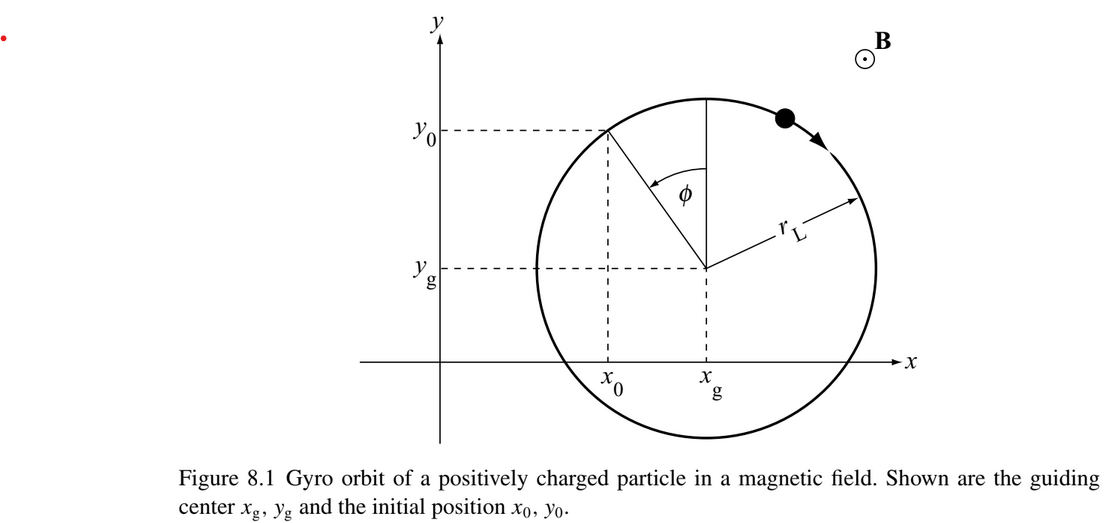
\includegraphics[width=\textwidth]{../../images/gyromotion_coordinates.png}
    \caption{Coordinates for gyromotion (extracted from Plasma Physics and Fusion Energy, J. P. Freidberg).}
    \label{fig:gyromotion_coordiantes}
\end{figure}

\label{sec:only_B_field}
Let's orient our coordinate system such that $\Bvec$ points in the $\evec_z$ direction. Thus, the equations of motion are
\begin{subequations}
\begin{alignat}{2}
    &\frac{d v_x}{dt} = \frac{eB}{m} v_y  \qquad && v_x(0) = v_\perp \cos(\phi), \label{eq:only_B_1} \\
    &\frac{d v_y}{dt} = -\frac{eB}{m} v_x  \qquad && v_y(0) = v_\perp \sin(\phi), \label{eq:only_B_2} \\
    &\frac{d v_z}{dt} = 0  \qquad && v_z(0) = v_{||}. \label{eq:only_B_3}
\end{alignat}
\end{subequations}
The $z$ component is decoupled from the rest and has a trivial solution. For the other two components, we begin by taking the time derivative of \cref{eq:only_B_2}. Thus
\begin{equation}
    \frac{d^2 v_y}{dt^2} = -\frac{eB}{m} \frac{d v_x}{dt} = -w_c^2 v_y,
\end{equation}
where $w_c = |e|B/m$ is the gyro frequency. We know that the general solution to the above is $v_y = c_1 \cos(w_c t) + c_2 \sin(w_c t)$. If we use the ICs and assume ions, we have
\begin{equation}
\label{eq:vel_gyro_y}
    v_y = -v_\perp \sin(w_ct - \phi).
\end{equation}
Integrating \cref{eq:only_B_1} then gives
\begin{equation}
\label{eq:vel_gyro_x}
    v_x = v_\perp \cos(w_c t - \phi).
\end{equation}
The final solution, for either positive or negative charges, can be written as
\begin{align}
\label{eq:vel_gyro}
    v^{(c)}_x &= v_\perp \cos(w_c t \pm \phi) \nonumber \\
    v^{(c)}_y &= \pm v_\perp \sin(w_c t \pm \phi),
\end{align}
where upper signs correspond to a negative charge. Integrating the equations above leads to
\begin{align}
\label{eq:pos_gyro}
    x^{(c)} &= r_L \sin(w_c t \pm \phi) \nonumber \\
    y^{(c)} &= \mp r_L \cos(w_c t \pm \phi).
\end{align}
where $r_L = v_\perp/w_c$ is the gyro radius.

%--------------------------------------------
\subsection{Both $\Evec$ and $\Bvec$ fields}
%--------------------------------------------
\label{sec:E_and_B_field}
Let's orient our coordinate system such that $\Bvec$ still points along $\evec_z$. The equations of motion are
\begin{subequations}
\label{eq:single_particle_motion_EcrossB_temp1}
\begin{alignat}{2}
    &\frac{d v_x}{dt} = \frac{eE_x}{m} + \frac{eB}{m} v_y  \qquad && v_x(0) = v_\perp \cos(\phi) + \frac{E_y}{B}, \label{eq:E_and_B_1} \\
    &\frac{d v_y}{dt} = \frac{eE_y}{m} - \frac{eB}{m} v_x  \qquad && v_y(0) = v_\perp \sin(\phi) - \frac{E_x}{B}, \label{eq:E_and_B_2} \\
    &\frac{d v_z}{dt} = \frac{e E_{||}}{m}  \qquad && v_z(0) = v_{||}, \label{eq:E_and_B_3}
\end{alignat}
\end{subequations}
where we have chosen the given initial conditions simply to facilitate the math. Again, the z component is decoupled from the rest and has the trivial solution $v_z = v_{||} +  (eE_{||}/m) t$. Thus, \cref{eq:single_particle_motion_vel_general} for the $x$ and $y$ components are
\begin{align}
    \label{eq:single_particle_motion_EcrossB_temp2}
    v_x &= v_x^{(c)} + v^{(g)}_x, \nonumber \\
    v_y &= v_y^{(c)} + v^{(g)}_y.
\end{align}
We assume $v^{(g)}_x$ and $v^{(g)}_y$ are time independent. Using \cref{eq:single_particle_motion_EcrossB_temp2} in \cref{eq:single_particle_motion_EcrossB_temp1} we obtain
\begin{align}
    0 &= \frac{eE_x}{m} + \frac{eB}{m}v^{(g)}_y \nonumber \\
    0 &= \frac{eE_y}{m} - \frac{eB}{m}v^{(g)}_x.
\end{align}
Thus, $v^{(g)}_x = E_y/B$ and $v^{(g)}_y = -E_x/B$, which in vector notation can be expressed as
\begin{equation}
    \vvec^{(g)}_E = \frac{\Evec \times \Bvec}{B^2}.
\end{equation}

%-------------------------------------------------------------------------------
\section{Non-uniform $\Bvec$ field}
%-------------------------------------------------------------------------------
%--------------------------------------------
\subsection{Change in magnitude along perpendicular directions}
%--------------------------------------------
The magnetic field still points in the $\evec_z$ direction, but its magnitude changes in directions perpendicular to $\evec_z$: $B = B(q_x,q_y)$. The equations of motion are
\begin{subequations}
\begin{alignat}{2}
    &\frac{d v_x}{dt} = \frac{eB(x,y)}{m} v_y  \qquad && v_x(0) = v_\perp \cos(\phi) -\frac{v^2_\perp}{2 w_c} \left . \frac{\partial B}{\partial q_y} \right |_{x_g,y_g} \frac{1}{B(x_g,y_g)}, \label{eq:nonuniB_1} \\
    &\frac{d v_y}{dt} = -\frac{eB(x,y)}{m} v_x  \qquad && v_y(0) = v_\perp \sin(\phi) + \frac{v^2_\perp}{2 w_c} \left . \frac{\partial B}{\partial q_x} \right |_{x_g,y_g} \frac{1}{B(x_g,y_g)}, \label{eq:nonuniB_2} \\
    &\frac{d v_z}{dt} = 0  \qquad && v_z(0) = v_{||}. \label{eq:nonuniB_3}
\end{alignat}
\end{subequations}
In the above, the $x$ and $y$ in $B(x,y)$ are the perpendicular components of the particle's position. The $v_z$ component is decoupled from the rest and has a trivial solution. Thus, \cref{eq:single_particle_motion_vel_general,eq:single_particle_motion_pos_general} for the $x$ and $y$ components are
\begin{equation}
    \label{eq:single_particle_motion_vel_Bmag_change_perp_1}
    v_x = v_x^{(c)} + v_x^{(g)},
\end{equation}
\begin{equation}
    \label{eq:single_particle_motion_vel_Bmag_change_perp_2}
    v_y = v_y^{(c)} + v_y^{(g)},
\end{equation}
\begin{equation}
    \label{eq:single_particle_motion_pos_Bmag_change_perp_1}
    x = x^{(c)} + x^{(g)},
\end{equation}
\begin{equation}
    \label{eq:single_particle_motion_pos_Bmag_change_perp_2}
    y = y^{(c)} + y^{(g)}.
\end{equation}

We begin by employing a Taylor-series expansion for the magnetic field
\begin{equation}
    B(x,y) = B(x_g, y_g) + \left . \frac{\partial B}{\partial q_x} \right |_{x_g,y_g} x^{(c)} + \left . \frac{\partial B}{\partial q_y} \right |_{x_g,y_g} y^{(c)} + ...
\end{equation}
Thus, \cref{eq:nonuniB_1,eq:nonuniB_2} are now
\begin{equation}
    \frac{ d v_x}{dt} = \frac{e B(x_g,y_g)}{m} v_y + \frac{e}{m} \left ( \left . \frac{\partial B}{\partial q_x} \right|_{x_g,y_g} x^{(c)} + \left . \frac{\partial B}{\partial q_y} \right |_{x_g,y_g} y^{(c)} \right) v_y
\end{equation}
\begin{equation}
    \frac{ d v_y}{dt} = -\frac{e B(x_g,y_g)}{m} v_x + \frac{e}{m} \left ( \left . \frac{\partial B}{\partial q_x} \right|_{x_g,y_g} x^{(c)} + \left . \frac{\partial B}{\partial q_y} \right |_{x_g,y_g} y^{(c)} \right ) v_x.
\end{equation}
As before, we assume $v_x^{(g)}$, $v_y^{(g)}$ are time independent. Also, for simplicity we assume ions only. Plugging in \cref{eq:single_particle_motion_vel_Bmag_change_perp_1,eq:single_particle_motion_vel_Bmag_change_perp_2} into the above, we get
\begin{equation}
    0 = B(x_g,y_g) v_y^{(g)} + \left ( \left . \frac{\partial B}{\partial q_x} \right|_{x_g,y_g} x^{(c)} + \left . \frac{\partial B}{\partial q_y} \right |_{x_g,y_g} y^{(c)} \right) \left ( v_y^{(c)} + v_y^{(g)} \right),
\end{equation}
\begin{equation}
    0 = -B(x_g,y_g) v_x^{(g)} + \left ( \left . \frac{\partial B}{\partial q_x} \right|_{x_g,y_g} x^{(c)} + \left . \frac{\partial B}{\partial q_y} \right |_{x_g,y_g} y^{(c)} \right ) \left ( v_x^{(c)} + v_x^{(g)} \right ).
\end{equation}
We assume $v_x^{(g)} \ll v_x^{(c)}$ and $v_y^{(g)} \ll v_y^{(c)}$. Thus, the above becomes
\begin{equation}
    \label{eq:single_particle_motion_Bmag_change_perp_temp1}
    0 = B(x_g,y_g) v_y^{(g)} + \left ( \left . \frac{\partial B}{\partial q_x} \right|_{x_g,y_g} x^{(c)} + \left . \frac{\partial B}{\partial q_y} \right |_{x_g,y_g} y^{(c)} \right) v_y^{(c)},
\end{equation}
\begin{equation}
    \label{eq:single_particle_motion_Bmag_change_perp_temp2}
    0 = -B(x_g,y_g) v_x^{(g)} + \left ( \left . \frac{\partial B}{\partial q_x} \right|_{x_g,y_g} x^{(c)} + \left . \frac{\partial B}{\partial q_y} \right |_{x_g,y_g} y^{(c)} \right ) v_x^{(c)}.
\end{equation}
We now use the definitions in \cref{eq:vel_gyro} and \cref{eq:pos_gyro}. For example, with those definitions we can show that 
\begin{align}
     x^{(c)} v_y^{(c)} &= \left[ r_L \sin (w_c t - \phi) \right] \left[ -v_\perp \sin (w_ct - \phi) \right] \nonumber \\
    & = -\frac{ v^2_\perp}{w_c} \sin^2(w_c t - \phi) \nonumber \\
    & = -\frac{ v^2_\perp}{2 w_c} \{1 - \cos [ 2 (w_c t - \phi)] \}
\end{align}
Similar derivations can be carried out for $y^{(c)} v_y^{(c)}$, $x^{(c)} v_x^{(c)}$, and $y^{(c)} v_x^{(c)}$. Thus, \cref{eq:single_particle_motion_Bmag_change_perp_temp1,eq:single_particle_motion_Bmag_change_perp_temp2} become 
\begin{multline}
    0 = B(x_g,y_g) v_y^{(g)} -\frac{ v^2_\perp}{2 w_c} \left . \frac{\partial B}{\partial q_x} \right |_{x_g,y_g} \{1 - \cos [ 2 (w_c t - \phi)] \} \\
    - \frac{ v^2_\perp}{2 w_c} \left .\frac{\partial B}{\partial q_y} \right |_{x_g,y_g} \sin [ 2(w_ct - \phi)],
\end{multline}
\begin{multline}
    0 = -B(x_g,y_g) v_x^{(g)} -\frac{ v^2_\perp}{2 w_c} \left . \frac{\partial B}{\partial q_x} \right |_{x_g,y_g} \sin [ 2 (w_c t - \phi)] \\
    - \frac{ v^2_\perp}{2 w_c} \left .\frac{\partial B}{\partial q_y} \right |_{x_g,y_g} \{ 1 + \cos [ 2(w_ct - \phi)] \}.
\end{multline}
It can be shown that the oscillatory terms containing the sines and cosines can be neglected. If it was not possible to neglect those terms, then the assumption that $v^{(g)}_x$, $v^{(g)}_y$ are time independent would not hold. Thus,
\begin{subequations}
\begin{alignat}{2}
    0 &= B(x_g,y_g) v_y^{(g)} - \frac{ v^2_\perp}{2 w_c} \left . \frac{\partial B}{\partial q_x} \right |_{x_g,y_g} \nonumber \\
    0 &= -B(x_g,y_g) v_x^{(g)} -\frac{ v^2_\perp}{2 w_c} \left . \frac{\partial B}{\partial q_y} \right |_{x_g,y_g} . 
\end{alignat}
\end{subequations}
Solving for the guiding center velocities, we finally have
\begin{align}
    v_x^{(g)} &= -\frac{v^2_\perp}{2 w_c} \left . \frac{\partial B}{\partial q_y} \right |_{x_g,y_g} \frac{1}{B(x_g,y_g)} \nonumber \\
    v_y^{(g)} &= \frac{v^2_\perp}{2 w_c} \left . \frac{\partial B}{\partial q_x} \right |_{x_g,y_g} \frac{1}{B(x_g,y_g)} . 
\end{align}
In vector notation, this is written as
\begin{equation}
    \vvec^{(g)}_{\nabla B} = \mp \frac{v^2_\perp}{2 w_c} \frac{ \Bvec \times \nabla B }{B^2}.
\end{equation}
In the above, the fields and $w_c$ are evaluated at $(x_g,y_g)$.

%--------------------------------------------
\subsection{Change in magnitude along parallel directions}
%--------------------------------------------
Ideally, one would introduce a gradient along the parallel direction to the magnetic field, that is, one would have $\Bvec = B(q_z) \evec_z$. However, due to Gauss's law, this is too restrictive and instead we generalize and use $\Bvec = B_x \evec_x + B_z \evec_z$, where $B_x = B_x(q_x,q_z)$ and $B_z = B_z(q_x,q_z)$. Thus, the equations of motion are
\begin{align}
    \frac{dv_x}{dt} &= \frac{e}{m} v_y B_z(x,z) , \label{eq:par_grad_vx_inter}\\
    \frac{dv_y}{dt} &= -\frac{e}{m} [v_x B_z(x,z) - v_z B_x(x,z)] , \label{eq:par_grad_vy_inter}\\
    \frac{dv_z}{dt} &= -\frac{e}{m} v_y B_x(x,z) \label{eq:par_grad_vz_inter}.
\end{align}
However, the $z$ direction no longer corresponds to the parallel direction, since the magnetic field also has a component along the $x$ direction. To account for this, we will introduce a rotating reference frame, in which one of the axis will always be aligned with the magnetic field vector, and thus would denote the parallel direction. In the original static reference frame the unit vectors are $(\evec_x, \evec_y, \evec_z)$ and the velocity components are $(v_x, v_y, v_x)$, whereas in this new rotating reference frame the unit vectors are $(\evec_{\perp1}, \evec_{\perp2}, \bvec)$ and the velocity components are $(v_{\perp1}, v_{\perp2}, v_{||})$. 

The rotating reference frame is described by the rotation matrix
\begin{equation}
    \Qvec(t) = \begin{bmatrix} b_x & 0 & b_z \\ 0 & 1 & 0 \\ b_z & 0 & -b_x \end{bmatrix},
\end{equation}
where $b_x = b_x(t)$ and $b_y = b_y(t)$ are given by
\begin{equation}
    b_x = \frac{B_x(x,z)}{B(x,z)} \qquad b_z = \frac{B_z(x,z)}{B(x,z)} \label{eq:bvec_components}
\end{equation}
In the above, $B(x,z) = [ B_x^2(x,z) + B_z^2(x,z) ]^{1/2}$. As an example, the matrix above leads to the following transformations for the unit vectors and velocities in the rotating reference frame 
\begin{align}
    \bvec &= b_x \evec_x + b_z \evec_z \\
    \evec_{\perp2} &= \evec_y \\
    \evec_{\perp1} &= b_z \evec_x - b_x \evec_z = \evec_{\perp2} \times \bvec,
\end{align}
\begin{align}
    v_{||} &= b_x v_x + b_z v_z \label{eq:par_grad_vel_trans_1}\\
    v_{\perp2} &= v_y \label{eq:par_grad_vel_trans_2}\\
    v_{\perp1} &= b_z v_x - b_x v_z. \label{eq:par_grad_vel_trans_3}
\end{align}
Using the transformation rule for the acceleration of a particle, but for some reason neglecting the coriollis and centrifugal forces, we obtain for the velocity derivatives
\begin{align}
    \frac{dv_{||}}{dt} &= \frac{dv_x}{dt} b_x + \frac{dv_z}{dt} b_z  - K v_{\perp1} \\
    \frac{dv_{\perp2}}{dt} &= \frac{dv_y}{dt}\\
    \frac{dv_{\perp1}}{dt} &= \frac{dv_x}{dt} b_z - \frac{dv_z}{dt} b_x + K v_{||},
\end{align}
where $K = K(t)$ is given by $K = b_x db_z/dt - b_z db_x/dt$. Using \cref{eq:par_grad_vx_inter,eq:par_grad_vy_inter,eq:par_grad_vz_inter} in the above leads to
\begin{align}
    \frac{d v_{||}}{dt} &= \frac{e}{m} v_y [B_z(x,z) b_x - B_x(x,z) b_z] - Kv_{\perp1} \\
    \frac{dv_{\perp2}}{dt} &= -\frac{eB}{m} (v_x b_z - v_z b_x) \\
    \frac{dv_{\perp1}}{dt} &= \frac{e}{m} v_y [B_z(x,z) b_z + B_x(x,z) b_x] + Kv_{||} 
\end{align}
Using the definitions for $b_x$ and $b_z$ in \cref{eq:bvec_components}, as well as the expressions for $v_{\perp1}$, $v_{\perp2}$ in \cref{eq:par_grad_vel_trans_2,eq:par_grad_vel_trans_3}, we get
\begin{align}
    \frac{d v_{||}}{dt} &= -Kv_{\perp1}, \label{eq:par_grad_vpar_inter} \\
    \frac{dv_{\perp2}}{dt} &= -w_c v_{\perp1}, \label{eq:par_grad_v2_inter} \\
    \frac{dv_{\perp1}}{dt} &= w_c v_{\perp2} + K v_{||}, \label{eq:par_grad_v1_inter}
\end{align}
where $w_c = w_c(t)$ is given by $w_c = e B(x,z) / m$.

We now introduce a time transformation to simplify the equations above. To do so, we introduce the following variables
\begin{gather}
    \hat{v}_{||} = \hat{v}_{||}(\tau) \qquad \hat{v}_{\perp2} = \hat{v}_{\perp2}(\tau) \qquad \hat{v}_{\perp1} = \hat{v}_{\perp1}(\tau) \\
    \hat{x} = \hat{x}(\tau) \qquad \hat{z} = \hat{z}(\tau)
\end{gather}
such that
\begin{gather}
    v_{||} = \hat{v}_{||}(h(t)) \qquad v_{\perp2} = \hat{v}_{\perp2}(h(t)) \qquad v_{\perp1} = \hat{v}_{\perp1}(h(t)) \\
    x = \hat{x}(h(t)) \qquad z = \hat{z}(h(t)).
\end{gather}
The function $h(t)$ is given by
\begin{equation}
    h(t) = \int_0^t w_c(t') dt'.
\end{equation}
We also show that
\begin{equation}
    b_x = \frac{B_x(x,z)}{B(x,z)} = \frac{B_x(\hat{x}(h(t)),\hat{z}(h(t)))}{B(\hat{x}(h(t)),\hat{z}(h(t)))},
\end{equation}
and thus
\begin{equation}
    \frac{db_x}{dt} = \frac{dh(t)}{dt} \frac{d}{d\tau} \left [ \frac{B_x(\hat{x},\hat{z})}{B(\hat{x},\hat{z})} \right ]_{\tau = h(t)} = w_c \left .\frac{d \hat{b}_x}{d\tau} \right|_{\tau = h(t)},
\end{equation}
where $\hat{b}_x =\hat{b}_x(\tau)$ is given by $\hat{b}_x= B_x(\hat{x},\hat{z}) / B(\hat{x},\hat{z})$. The analogous holds for $b_z$. This allows us to write
\begin{equation}
    K = w_c \left ( \hat{b}_x \frac{d\hat{b}_z}{dt} - \hat{b}_z \frac{d\hat{b}_x}{dt} \right)_{\tau = h(t)} = w_c \left. \hat{K} \right |_{\tau = h(t)},
\end{equation}
where $\hat{K} = \hat{K}(\tau)$ is given by $\hat{K} = \hat{b}_x d\hat{b}_z/d\tau - \hat{b}_z d\hat{b}_x/d\tau$. With these transformation, \cref{eq:par_grad_vpar_inter,eq:par_grad_v2_inter,eq:par_grad_v1_inter} are re-written as
\begin{align}
    \frac{d\hat{v}_{||}}{d\tau} &= -\hat{K} \hat{v}_{\perp1},\\
    \frac{d\hat{v}_{\perp2}}{d\tau} &= -\hat{v}_{\perp1},\\
    \frac{d\hat{v}_{\perp1}}{d\tau} &= \hat{v}_{\perp2} + \hat{K} \hat{v}_{||}.
\end{align}

We now simplify $B_z$ so that $B_z = B_z(q_z)$. To be consistent with Gauss's law, we require $B_x = B_x(q_x,q_y)$ where $B_x = -q_x dB_z/dq_z$. With these simplified forms, we have
\begin{align}
    \hat{K} &= -\hat{b}_z^2 \frac{d}{d\tau} \left ( \frac{\hat{b}_x}{\hat{b}_z} \right ) \\
    &= -\frac{B_z^2(\hat{z})}{B^2(\hat{x},\hat{z})} \frac{d}{d\tau} \left ( \frac{B_x(\hat{x},\hat{z})}{B_z(\hat{z})} \right ) \\
    &= \frac{B_z^2(\hat{z})}{B^2(\hat{x},\hat{z})} \frac{d}{d\tau} \left [ \hat{x}  \left ( \frac{1}{B_z} \frac{dB_z}{dq_z} \right )_{q_z = \hat{z}} \right ].
\end{align}
We now use the long-thin approximation. For this approximation, we assume that $B_x / B_z \ll 1$, and also that $\frac{1}{B_z} \frac{dB_z}{dq_z}$ changes very slowly. We thus have
\begin{equation}
\label{eq:par_grad_k_inter}
    \hat{K} \approx \frac{d \hat{x}}{d\tau} \left ( \frac{1}{B_z} \frac{dB_z}{dq_z} \right)_{q_z = \hat{z}}.
\end{equation}
Also, using the long-thin approximation in \cref{eq:par_grad_vel_trans_1,eq:par_grad_vel_trans_3} allows us to write
\begin{align}
    v_{||} &\approx v_z = \frac{dz}{dt} = \left ( \frac{d\hat{z}}{d\tau} \right)_{\tau = h(t)} w_c \\
    v_{\perp1} & \approx v_x = \frac{dx}{dt} = \left ( \frac{d \hat{x}}{d\tau} \right)_{\tau = h(t)} w_c.
\end{align}
Evaluating the above at $t = h^{-1}(\tau)$, and defining $\hat{w}_c(\tau)$ from $w_c = \hat{w}_c(h(t))$, we obtain
\begin{align}
    \hat{v}_{||} &\approx  \frac{d\hat{z}}{d\tau}  \hat{w}_c \\
    \hat{v}_{\perp1} & \approx \frac{d \hat{x}}{d\tau} \hat{w}_c.
\end{align}
We also note that
\begin{equation}
    \frac{d B_z(\hat{z})}{d\tau} = \left ( \frac{dB_z}{dq_z} \right)_{q_z = \hat{z}} \frac{d \hat{z}}{d\tau}.
\end{equation}
Using the expressions above in \cref{eq:par_grad_k_inter}, one can approximate $\hat{K}$ using either of the two forms below
\begin{equation}
    \hat{K} \approx \frac{\hat{v}_{\perp1}}{\hat{w}_c B_z(\hat{z})} \left ( \frac{dB_z}{dq_z} \right)_{q_z = \hat{z}} \approx \frac{\hat{v}_{\perp1}}{\hat{v}_{||} B_z(\hat{z})} \frac{dB_z(\hat{z})}{d\tau} .
\end{equation}
We thus write the governing equations for the velocities as
\begin{align}
    \frac{d\hat{v}_{||}}{d\tau} &= -\frac{\hat{v}^2_{\perp1}}{\hat{w}_c B_z(\hat{z})} \left ( \frac{dB_z}{dq_z} \right)_{q_z = \hat{z}} ,\label{eq:par_grad_vpar_thin}\\
    \frac{d\hat{v}_{\perp2}}{d\tau} &= -\hat{v}_{\perp1}, \label{eq:par_grad_v2_thin} \\
    \frac{d\hat{v}_{\perp1}}{d\tau} &= \hat{v}_{\perp2} + \frac{\hat{v}_{\perp1}}{B_z(\hat{z})} \frac{dB_z(\hat{z})}{d\tau}. \label{eq:par_grad_v1_thin}
\end{align}

We now assume the solution for the perpendicular velocities is of the form
\begin{align}
    \hat{v}_{\perp1} &= \hat{v}_\perp \cos [\tau + \hat{\epsilon}] \\
    \hat{v}_{\perp2} &= -\hat{v}_\perp \sin [\tau + \hat{\epsilon}],
\end{align}
where $\hat{v}_\perp = \hat{v}_\perp(\tau)$ and $\hat{\epsilon} = \hat{\epsilon}(\tau)$. Plugging these two assumed solutions into \cref{eq:par_grad_v2_thin,eq:par_grad_v1_thin}, and using some simple algebra, gives
\begin{equation}
    \frac{d\hat{v}_\perp}{d\tau} = \frac{\hat{v}_\perp}{2 B_z(\hat{z})} \frac{dB_z(\hat{z})}{d\tau} \left \{ 1 + \cos [2 (\tau + \hat{\epsilon})] \right \}.
\end{equation}
The above can be re-arranged and expressed as
\begin{equation}
\label{eq:par_grad_mu_evol}
    \frac{d \ln \hat{\mu}}{d\tau} = \frac{d \ln B_z(\hat{z}) }{d\tau} \cos [2 (\tau + \hat{\epsilon})],
\end{equation}
where $\hat{\mu} = \hat{\mu}(\tau)$ is the adiabatic invariant, and is given by
\begin{equation}
    \hat{\mu} = \frac{m \hat{v}^2_\perp}{2 B_z(\hat{z})}.
\end{equation}
Integrating \cref{eq:par_grad_mu_evol} from $\tau_1$ to $\tau_2$ gives
\begin{equation}
    \ln \hat{\mu}(\tau_2) - \ln \hat{\mu}(\tau_1) = \left . \ln [B_z(\hat{z})] \cos [2(\tau + \hat{\epsilon})] \right |^{\tau_2}_{\tau_1} + \int_{\tau_1}^{\tau_2} 2 \ln [ B_z(\hat{z}) ] \sin [2(\tau + \hat{\epsilon})] d\tau.
\end{equation}
Picking $\tau_1$ and $\tau_2$ such that $[\tau_2 + \hat{\epsilon}(\tau_2)] - [\tau_1 + \hat{\epsilon}(\tau_1)] = 2 \pi$, and assuming $B(\hat{z})$ doesn't change significantly from $\tau_1$ to $\tau_2$, gives $\hat{\mu}(\tau_2) = \hat{\mu}(\tau_1)$, that is, $\hat{\mu}$ is constant over one gyro-period. One can also define
\begin{equation}
    \mu = \frac{m v_\perp^2}{2B_z(z)}
\end{equation}
where $\mu = \mu(t)$ and $v_\perp = v_\perp(t)$. Given that $v_\perp = \hat{v}_\perp(h(t))$, we have $\mu = \hat{\mu}(h(t))$. Thus, $\hat{\mu}(\tau_2) = \hat{\mu}(\tau_1)$ translates to $\mu(t_2) = \mu(t_1)$, where $t_2 = h^{-1}(\tau_2)$ and $t_1 = h^{-1}(\tau_1)$.

Finally, we focus not on the perpendicular velocities but the parallel velocity. Plugging-in the assumed solutions in the governing \cref{eq:par_grad_vpar_thin} gives
\begin{equation}
    \frac{d\hat{v}_{||}}{d\tau} = -\frac{\hat{v}^2_{\perp}}{2\hat{w}_c B_z(\hat{z})} \left ( \frac{dB_z}{dq_z} \right)_{q_z = \hat{z}} \{ 1 + \cos [2(\tau + \hat{\epsilon})] \}.
\end{equation}
We now average the above from $\tau_1$ to $\tau_2$ while assuming $B(\hat{z})$, $d\hat{v}_{||}/d\tau$ and $\hat{v}^2_\perp$ do not change significantly during that time scale. Note that since this is an average, we are not just integrating from $\tau_1$ to $\tau_2$, but we are also dividing by $\tau_2 - \tau_1$. After  averaging, we obtain
\begin{equation}
    \frac{d\hat{v}_{||}}{d\tau} = -\frac{\hat{v}^2_{\perp}}{2\hat{w}_c B_z(\hat{z})} \left ( \frac{dB_z}{dq_z} \right)_{q_z = \hat{z}} .
\end{equation}
or
\begin{equation}
    m \frac{d\hat{v}_{||}}{d\tau} = -\frac{\hat{\mu}}{\hat{w}_c} \left ( \frac{dB_z}{dq_z} \right)_{q_z = \hat{z}} .
\end{equation}
Converting back to time $t$ gives
\begin{equation}
    m \frac{dv_{||}}{dt} = -\mu \left ( \frac{dB_z}{dq_z} \right)_{q_z = z} .
\end{equation}


%--------------------------------------------
\subsection{Change in direction}
%--------------------------------------------
Rather than writing \cref{eq:single_particle_motion} in terns if its components as done in previous sections, we leave the equation in vector. Expressing the velocity as $\vvec = \vvec_\perp + v_{||} \bvec$ and assuming no electric field, we write \cref{eq:single_particle_motion} as
\begin{equation}
    \frac{d}{dt} ( \vvec_\perp + v_{||} \bvec) = \mp w_c (\vvec_\perp + v_{||} \bvec ) \times \bvec,
\end{equation}
where upper sign corresponds to negative charge and lower sign to positive charge. For simplicity we will assume positively charged particles only. We then cross both sides of the above by $\bvec$, that is
\begin{equation}
    \bvec \times \left \{ \left [ \frac{d}{dt} ( \vvec_\perp + v_{||} \bvec) - w_c ( \vvec_\perp + v_{||} \bvec) \times \bvec \right ] \times \bvec \right \} = 0.
\end{equation}
The above is simplified using the following three manipulations
\begin{align}
    \bvec \times \left \{ \left [ w_c ( \vvec_\perp + v_{||} \bvec) \times \bvec \right] \times \bvec \right \} &= \bvec \times \left \{ \left [ w_c \vvec_\perp \times \bvec \right] \times \bvec \right \} \nonumber \\
    & = -\bvec \times \left \{ w_c \vvec_\perp ( \bvec \cdot \bvec) - \bvec (\bvec \cdot w_c \vvec_\perp ) \right \} \nonumber \\
    & = w_c \vvec_\perp \times \bvec.
\end{align}
\begin{equation}
    \bvec \times \left \{ \left [ \frac{d\vvec_\perp}{dt} \right] \times \bvec \right \} = \frac{d \vvec_\perp}{dt}( \bvec \cdot \bvec) - \bvec \left(\bvec \cdot \frac{d\vvec_\perp}{dt} \right ) = \left ( \frac{d \vvec_\perp}{dt} \right)_\perp.
\end{equation}
\begin{align}
    \bvec \times \left \{ \left [ \frac{d v_{||} \bvec}{dt} \times \bvec \right] \right \} &= v_{||} \bvec \times \left \{ \left [ \frac{ d\bvec}{dt} \times \bvec \right] \right \} \nonumber \\
    & = v_{||} \left [ \frac{d \bvec}{dt} ( \bvec \cdot \bvec) - \bvec \left ( \bvec \cdot \frac{d \bvec}{dt} \right ) \right ] \nonumber \\
    & = v_{||} \left [ \frac{d \bvec}{dt} - \bvec \left ( \frac{1}{2} \cdot \frac{d \bvec \cdot \bvec}{dt} \right ) \right ] \nonumber \\
    & = v_{||} \frac{d \bvec}{dt}
\end{align}
Thus, we have
\begin{equation}
\label{eq:curvature_1}
    \left ( \frac{ d \vvec_\perp}{dt} \right)_\perp - w_c \vvec_\perp \times \bvec = -v_{||} \frac{d\bvec}{dt}.
\end{equation}
As shown in Freidberg
\begin{equation}
    \frac{d \bvec(\xvec(t))}{dt} = \frac{d \xvec(t)}{dt} \cdot \nabla \bvec = \vvec \cdot \nabla \bvec = \vvec_\perp \cdot \nabla \bvec + v_{||} \bvec \cdot \nabla \bvec,
\end{equation}
where $\nabla \bvec$ is evaluated at $\xvec = \xvec(t)$. Thus, \cref{eq:curvature_1} becomes
\begin{equation}
\label{eq:curvature_2}
    \left ( \frac{ d \vvec_\perp}{dt} \right)_\perp - w_c \vvec_\perp \times \bvec = -v_{||} \vvec_\perp \cdot \nabla \bvec - v_{||}^2 \bvec \cdot \nabla \bvec.
\end{equation}
As was done for the other drifts, we assume the solution is of the form $\vvec_\perp = \vvec^{(c)} + \vvec^{(g)}$, where we assume again that $\vvec^{(g)}$ is time independent. The term $\vvec^{(c)}$ corresponds to gyromotion in a rotating reference frame, and is thus given by 
\begin{equation}
    \vvec^{(c)} = v^{(c)}_{\perp1} \evec_{\perp1} + v^{(v)}_{\perp2} \evec_{\perp2},
\end{equation}
where $\evec_{\perp1}$ and $\evec_{\perp2}$ are orthogonal to $\bvec$ and thus rotate in time. $v^{(c)}_{\perp1}$ is given by \cref{eq:vel_gyro_x} and $v^{(c)}_{\perp2}$ by \cref{eq:vel_gyro_y}. We note that, in the non-rotating reference frame, $\vvec^{(c)}$ is expressed as $\vvec^{(c)} = v^{(c)}_x \evec_x + v^{(c)}_y \evec_y + v^{(c)}_z \evec_z$. We now prove that $\vvec_\perp^{(c)}$ is the solution to the two terms on the left-hand side of \cref{eq:curvature_2}. To show this we first use the transformation rule for the acceleration of a particle in a rotating reference frame, but for some reason ignore the coriollis and centrifugal terms. Thus
\begin{align}
    \frac{d \vvec^{(c)}}{dt} &= \frac{dv^{(c)}_x}{dt} \evec_x + \frac{dv^{(c)}_y}{dt} \evec_y + \frac{dv^{(c)}_z}{dt} \evec_z \nonumber \\ &= \frac{dv^{(c)}_{\perp1}}{dt} \evec_{\perp1} + \frac{dv^{(c)}_{\perp2}}{dt} \evec_{\perp2} + 2\Omega \times \vvec^{(c)}.
\end{align}
We do not allow the rotating reference frame to rotate about the $\bvec$ axis. Thus, $\Omega = \Omega_{\perp1} \evec_{\perp1} + \Omega_{\perp2} \evec_{\perp2}$. Given that $\Omega$ and $\vvec^{(c)}$ are in the same plane, $\Omega \times \vvec^{(c)}$ must point in the $\bvec$ direction. Thus, 
\begin{equation}
    \left ( \frac{d \vvec^{(c)}}{dt} \right)_\perp = \frac{dv^{(c)}_{\perp1}}{dt} \evec_{\perp1} + \frac{dv^{(c)}_{\perp2}}{dt} \evec_{\perp2}.
\end{equation}
This allows us to show that 
\begin{equation}
    \left ( \frac{d \vvec^{(c)}}{dt} \right)_\perp - w_c \vvec^{(v)} \times \bvec = \frac{dv^{(c)}_{\perp1}}{dt} \evec_{\perp1} + \frac{dv^{(c)}_{\perp2}}{dt} \evec_{\perp2} - w_c v^{(c)}_{\perp2} \evec_{\perp1} + w_c v^{(c)}_{\perp1} \evec_{\perp2} = 0.
\end{equation}
We now plug in $\vvec_\perp = \vvec^{(c)} + \vvec^{(g)}$ in \cref{eq:curvature_2} to obtain
\begin{equation}
\label{eq:curvature_3}
    -w_c \vvec^{(g)} \times \bvec = - v_{||} \vvec_\perp \cdot \nabla \bvec - v_{||}^2 \bvec \cdot \nabla \bvec.
\end{equation}
As explained in Freidberg, the term $v_{||} \vvec_\perp \cdot \nabla \bvec$ leads to small modifications of the gyro motion, but does not lead to a drift of the particles, and thus is ignored. Taking the cross product of \cref{eq:curvature_3} with $\bvec$ finally gives the curvature drift
\begin{equation}
    \vvec^{(g)}_\kappa = \pm \frac{v_{||}^2}{w_c} \frac{( \bvec \cdot \nabla \bvec ) \times \Bvec}{B}.
\end{equation}

We now show that, if we assume $\nabla \times \Bvec = 0$, the grad-B drift 
\begin{equation}
    \vvec^{(g)}_{\nabla B} = \mp \frac{v^2_\perp}{2 w_c} \frac{\Bvec \times \nabla B}{B^2}
\end{equation}
can be written in the same form as the curvature drift. We begin by showing that
\begin{equation}
    \Bvec \times \nabla B = \Bvec \times \nabla \left ( \Bvec \cdot \Bvec \right )^{1/2} = \Bvec \times \frac{1}{2B} \nabla \left ( \Bvec \cdot \Bvec \right ).
\end{equation}
We now use the vector identity $\nabla (\Bvec \cdot \Bvec ) = 2 \Bvec \times (\nabla \times \Bvec) + 2 \Bvec \cdot \nabla \Bvec$, and assume magnetic curl of zero to obtain
\begin{align}
    \Bvec \times \nabla B &= \Bvec \times \frac{1}{B} \Bvec \cdot \nabla \Bvec \nonumber \\
    &= \Bvec \times \bvec \cdot \nabla (B \bvec) \nonumber \\
    &= \Bvec \times \left (\bvec \cdot \nabla B \right ) \bvec + \Bvec \times B \left (\bvec \cdot \nabla \bvec \right ) \nonumber \\
    &= -B \left ( \bvec \cdot \nabla \bvec \right ) \times \Bvec.
\end{align}
Thus, the grab-B drift can be written as 
\begin{equation}
    \vvec^{(g)}_{\nabla B} = \pm \frac{v^2_\perp}{2 w_c} \frac{(\bvec \cdot \nabla \bvec) \times \Bvec}{B}.
\end{equation}

%-------------------------------------------------------------------------------
\section{Non-uniform $\Evec$ field}
%-------------------------------------------------------------------------------

%-------------------------------------------------------------------------------
\section{Time-varying $\Evec$ field}
%-------------------------------------------------------------------------------
Consider the scenario used in \cref{sec:E_and_B_field}, but with a time varying electric field. The equations of motion are
\begin{subequations}
\label{eq:time_var_E_temp1}
\begin{alignat}{2}
    &\frac{d v_x}{dt} = \frac{eE_x(t)}{m} + \frac{eB}{m} v_y  \qquad && v_x(0) = v_\perp \cos(\phi) + \frac{E_y(t)}{B} + \frac{m}{eB^2}\frac{dE_x(t)}{dt},  \\
    &\frac{d v_y}{dt} = \frac{eE_y(t)}{m} - \frac{eB}{m} v_x  \qquad && v_y(0) = v_\perp \sin(\phi) - \frac{E_x(t)}{B} + \frac{m}{eB^2}\frac{dE_y(t)}{dt},  \\
    &\frac{d v_z}{dt} = \frac{e E_{||}(t)}{m}  \qquad && v_z(0) = v_{||}, 
\end{alignat}
\end{subequations}
where again we chose the initial conditions simply to be consistent with the solution that we'll derive. The parallel velocity is independent of the perpendicular velocities, and we won't worry about it for now. To solve for the perpendicular velocities, we again assume the general solution is 
\begin{align}
\label{eq:time_var_temp2}
    v_x = v_x^{(gm)} + V_x \nonumber \\
    v_y = v_y^{(gm)} + V_y 
\end{align}
but now $V_x$ and $V_y$ are not time independent. We expand $V_i$ as $V_i = V^{(1)}_i +  V^{(2)}_i + ...$, where $V^{(\alpha)} \sim \epsilon V^{(\alpha-1)}$, and the small parameter $\epsilon$ follows from assuming 
\begin{equation}
\label{eq:time_var_E_temp3}
    \frac{1}{V^{(\alpha)}_i} \frac{d V^{(\alpha)}_i}{dt} \sim \epsilon w_c.
\end{equation}
That is, the time scale associated with the rate of change of all of the $V^{(\alpha)}_i$ components is much larger than the time scale of the gyromotion. In other words, we assume particles gyrate faster than how quickly their drift velocity changes. Using \cref{eq:time_var_temp2} in \cref{eq:time_var_E_temp1} leads to
\begin{align}
    \frac{dV_x^{(1)}}{dt} + \frac{dV_x^{(2)}}{dt} &= \frac{eE_x(t)}{m} + \frac{eB}{m} V_y^{(1)} + \frac{eB}{m} V_y^{(2)} \nonumber \\
    \frac{dV_y^{(1)}}{dt} + \frac{dV_y^{(2)}}{dt} &= \frac{eE_y(t)}{m} - \frac{eB}{m} V_x^{(1)} - \frac{eB}{m} V_x^{(2)}.
\end{align}
Collecting lowest order terms
\begin{align}
    0 &= \frac{eE_x(t)}{m} + \frac{eB}{m} V_y^{(1)}  \nonumber \\
    0 &= \frac{eE_y(t)}{m} - \frac{eB}{m} V_x^{(1)} ,
\end{align}
and thus $V^{(1)}_x = E_y(t)/B$ and $V^{(1)}_y = -E_x(t)/B$, which in vector notation is
\begin{equation}
    \Vvec^{(1)} = \frac{\Evec(t) \times \Bvec}{B^2}.
\end{equation}
Collecting first order terms 
\begin{align}
    \frac{dV_x^{(1)}}{dt} &=  \frac{eB}{m} V_y^{(2)} \nonumber \\
    \frac{dV_y^{(1)}}{dt} &=  -\frac{eB}{m} V_x^{(2)},
\end{align}
and thus $V_x^{(2)} = (m/eB^2)dE_x(t)/dt$ and $V_y^{(2)} = (m/eB^2) dE_y(t)/dt$, which in vector notation is
\begin{equation}
    \Vvec^{(2)} = \mp \frac{1}{w_c B}\frac{d\Evec_\perp}{dt}.
\end{equation}
We note that, by looking at the solutions for $V_x^{(1)}$ and $V_y^{(1)}$, the assumption in \cref{eq:time_var_E_temp3} is equivalent to stating that the electric field changes slowly. 

%-------------------------------------------------------------------------------
\section{Time-varying $\Bvec$ field}
%-------------------------------------------------------------------------------
Let's assume the magnetic field points in the $z$ direction again. Using Faraday's law, we have
\begin{equation}
    \left(\frac{\partial E_z}{\partial q_y} - \frac{\partial E_y}{\partial q_z} \right) \evec_x - \left(\frac{\partial E_z}{\partial q_x} - \frac{\partial E_x}{\partial q_z} \right) \evec_y + \left(\frac{\partial E_y}{\partial q_x} - \frac{\partial E_x}{\partial q_y} \right) \evec_z = -\frac{\partial B}{\partial t} \evec_z.
\end{equation}
To satisfy the above, we set $E_z = 0$, and $E_x = E_x(q_x,q_y,t)$, $E_y = E_y(q_x,q_y,t)$. That is, a time varying magnetic field requires a time and spatially varying electric field. 

We will further simplify our analysis by having $E_x = 0$ and $E_y = E_y(q_x,t)$. Thus, the equations of motion are
\begin{align}
    \frac{dv_x}{dt} &= \frac{eB(t)}{m} v_y \\
    \frac{dv_y}{dt} &= \frac{eE_y(x,t)}{m} - \frac{eB(t)}{m}v_x
\end{align}
The electric field is linearized using a Taylor-series expansion
\begin{align}
    \frac{dv_x}{dt} &= \frac{eB(t)}{m} v_y \\
    \frac{dv_y}{dt} &= \frac{e}{m}\left( E_y(x_g,t) + \left .\frac{\partial E_y}{\partial q_x} \right |_{x_g} r_x\right) - \frac{eB(t)}{m}v_x,
\end{align}
where $r_x = x - x_g$. We assume positive ions for simplicity and re-write the above as
\begin{align}
    \frac{dv_x}{dt} &= w_c v_y \\
    \frac{dv_y}{dt} &= \frac{w_c}{B(t)}\left( E_y(x_g,t) + \left .\frac{\partial E_y}{\partial q_x} \right |_{x_g} r_x\right) - w_c v_x.
\end{align}
where $w_c = w_c(t)$. We introduce new variables 
\begin{gather}
    \hat{v}_x = \hat{v}_x(\tau) \qquad \hat{v}_y = \hat{v}_y(\tau) \qquad \hat{x} = \hat{x}(\tau) \qquad \hat{x}_g = \hat{x}_g(\tau) \nonumber \\ \hat{r}_x = \hat{r}_x(\tau) \qquad \hat{E}_y = \hat{E}_y(q_x,\tau) \qquad \hat{B} = \hat{B}(\tau)
\end{gather}
such that 
\begin{gather}
    v_x(t) = \hat{v}_x(h(t)) \qquad
    v_y(t) = \hat{v}_y(h(t)) \qquad
    x(t) = \hat{x}(h(t)) \qquad
    x_g(t) = \hat{x}_g(h(t)) \nonumber \\
    r_x(t) = \hat{r}_x(h(t)) \qquad
    E_y(q_x,t) = \hat{E}_y(q_x,h(t)) \qquad
    B(t) = \hat{B}(h(t)).
\end{gather}
For the above
\begin{equation}
    h(t) = \int_0^t w_c(t') \, dt'.
\end{equation}
The equations of motion then become
\begin{align}
\label{eq:time_var_B_inter_1}
    \frac{d \hat{v}_x}{d \tau} &= \hat{v}_y \nonumber \\
    \frac{d \hat{v}_y}{d \tau} &= \frac{1}{\hat{B}(\tau)}\left( \hat{E}_y(\hat{x}_g,\tau) + \left .\frac{\partial \hat{E}_y}{\partial q_x} \right |_{\hat{x}_g} \hat{r}_x\right) - \hat{v}_x.
\end{align}
These are the equations we need to solve. To do so, we assume a form of the solution that is inspired by the previous section on time-dependent electric fields. That is, we assume the solution is of the form
\begin{align}
\label{eq:time_var_B_inter_2}
    \hat{v}_x &= \hat{v}_\perp \cos[\tau + \hat{\epsilon}] + \frac{\hat{E}_y(\hat{x}_g,\tau)}{\hat{B}(\tau)} \nonumber \\
    \hat{v}_y &= -\hat{v}_\perp \sin[\tau + \hat{\epsilon}]+ \frac{d}{d \tau} \left ( \frac{\hat{E}_y(\hat{x}_g,\tau)}{\hat{B}(\tau)} \right ).
\end{align}
where $\hat{v}_\perp = \hat{v}_\perp(\tau)$ and $\hat{\epsilon} = \hat{\epsilon}(\tau)$ are now time-dependent functions. As done before, we assume $\hat{r}_x = \hat{r}_x^{(gm)} + \hat{g}_x$, where $\hat{r}_x^{(gm)} = \hat{x}^{(gm)} - \hat{x}_g$, and $\hat{g}_x \sim \epsilon \hat{r}_x^{(gm)}$. The analogue of \cref{eq:pos_gyro} would be 
\begin{equation}
\label{eq:time_var_B_inter_3}
    \hat{x}^{(gm)} = \hat{x}_g + \hat{r}_L \sin [\tau + \hat{\epsilon}],
\end{equation}
where $\hat{r}_L = \hat{r}_L(\tau)$ is given by $\hat{r}_L = \hat{v}_\perp / \hat{w}_c$, and $\hat{w}_c = q\hat{B}(\tau)/m$. Plugging in \cref{eq:time_var_B_inter_2,eq:time_var_B_inter_3} in \cref{eq:time_var_B_inter_1} and using some algebra, leads to
\begin{equation}
\frac{d \ln \hat{\mu}}{d\tau} = \frac{d \ln \hat{B}(\tau)}{d\tau} \cos [ 2 (\tau + \hat{\epsilon}) ],
\end{equation}
where $\hat{\mu} = \hat{\mu}(\tau)$ is given by
\begin{equation}
    \hat{\mu} = \frac{m \hat{v}_\perp^2}{2\hat{B}(\tau)}.
\end{equation}
Integrating over one gyro-period, i.e.\@ from $\tau_1$ to $\tau_2$ such that $[\tau_2 + \epsilon(\tau_2)] - [\tau_1 + \epsilon(\tau_1)] = 2\pi$, gives
\begin{equation}
    \ln \hat{\mu}(\tau_2) - \ln \hat{\mu}(\tau_1) = \left. \ln [\hat{B}(\tau)] \cos [2 (\tau+\hat{\epsilon})] \right |_{\tau_1}^{\tau_2} + \int_{\tau_1}^{\tau_2} 2 \ln [\hat{B}(\tau)] \sin[2(\tau+\hat{\epsilon})] \, d\tau.
\end{equation}
Assuming $\hat{B}(\tau)$ doesn't change significantly from $\tau_1$ to $\tau_2$, then we have $\hat{\mu}(\tau_2) = \hat{\mu}(\tau_1)$, that is, $\hat{\mu}$ is constant over one gyro-period. On can also define
\begin{equation}
    \mu = \frac{m v_\perp^2}{2 B(t)}
\end{equation}
where $\mu = \mu(t)$ and $v_\perp = v_\perp(t)$. Given that $v_\perp = \hat{v}_\perp(h(t))$, we have $\mu = \hat{\mu}(h(t))$. Thus, $\hat{\mu}(\tau_2) = \hat{\mu}(\tau_1)$ translates to $\mu(t_2) = \mu(t_1)$, where $t_2 = h^{-1}(\tau_2)$ and $t_1 = h^{-1}(\tau_1)$.

As shown in the analysis above, for a time dependent magnetic field a drift of the following form is introduced
\begin{equation}
    \hat{V}_y = \frac{d}{d\tau} \left ( \frac{\hat{E}_y(\hat{x}_g,\tau)}{\hat{B}(\tau)} \right ).
\end{equation}
Converting back to time $t$
\begin{equation}
    V_y = \frac{1}{w_c} \frac{d}{dt} \left ( \frac{E_y(x_g,t)}{B(t)} \right ).
\end{equation}
For the more general case where $E_x = E_x(q_x,q_y,t)$ and $E_y = E_y(q_x,q_y,t)$ then
\begin{equation}
    \Vvec_p = \mp \frac{1}{w_c} \frac{d}{dt} \left ( \frac{\Evec_\perp}{B} \right ),
\end{equation}
where top sign is for electrons and bottom sign is for ions, and it is assumed that the electric field is evaluated at the gyro-center. For an even more general case where the magnetic field does not necessarily point in one direction,
\begin{equation}
    \Vvec_p = \mp \frac{1}{w_c} \bvec \times \frac{d\Vvec_E}{dt}.
\end{equation}

%--------------------------------------------------------------------------------------------------------------------------------------------
\chapter{Plasma parameters, time scales, and length scales}
%--------------------------------------------------------------------------------------------------------------------------------------------
A summary of fundamental time and length scales of plasmas in given in \cref{tb:plasma_time_scales,tb:plasma_length_scales}
\begin{table}[H]
\renewcommand{\arraystretch}{2.5}
\centering
\caption{Plasma time scales, for either electrons ($\alpha = e$) or ions ($\alpha = i$). }
\label{tb:plasma_time_scales}
 \begin{tabular}{l|l}
    Time scales & Formulas \\
    \hline
    Gyro period  & $\tau_{c\alpha} = \dfrac{2\pi}{w_{c\alpha}} \quad w_{c\alpha} = \dfrac{q_\alpha B}{m_\alpha}$ \\
    Plasma period & $\tau_{p\alpha} = \dfrac{2 \pi }{w_{p\alpha}} \quad w_{p\alpha} = \sqrt{\dfrac{n_\alpha q_\alpha^2}{m_\alpha \epsilon_0}}$
 \end{tabular}
\end{table}

\begin{table}[H]
\renewcommand{\arraystretch}{2.5}
\centering
\caption{Plasma length scales, for either electrons ($\alpha = e$) or ions ($\alpha = i$).}
\label{tb:plasma_length_scales}
 \begin{tabular}{l|l}
   Length scales & Formulas \\
   \hline
   Gyro radius  & $r_{c\alpha} = \dfrac{v_{T\alpha}}{w_{c\alpha}} = \dfrac{m v_{T\alpha}}{q_\alpha B}$ \\
   Debye length & $\lambda_{D\alpha} = \dfrac{v_{T\alpha}}{\sqrt{2} w_{p\alpha}} = \sqrt{ \dfrac{\epsilon_0 k_B T_\alpha}{ n_\alpha q_\alpha^2}}$ \\
   DeBroglie wave length & $\lambda_{B\alpha} = \dfrac{h}{\sqrt{\pi} m_\alpha v_{T\alpha}}$ \\
   Sphere radius & $a_\alpha = \left ( \dfrac{3}{4 \pi n_\alpha} \right )^{1/3}$
\end{tabular}
\end{table}

\begin{itemize}
\item Thermal velocity:
\begin{equation}
v_{T_\alpha} = \sqrt{\frac{2 k_B T_\alpha}{m_\alpha}}
\end{equation}

\item Total Debye length:
\begin{equation}
    \frac{1}{\lambda_D^2} = \sum_\alpha \frac{1}{\lambda_{D\alpha}^2}.
\end{equation}

\item Plasma parameter
\begin{equation}
    \Lambda_\alpha = \frac{4}{3} \pi \lambda_{D\alpha}^3 n_\alpha
\end{equation}

\item Quantum plasma parameter
\begin{equation}
    \chi_\alpha = \frac{4}{3} \pi \lambda_{B\alpha}^3 n_\alpha
\end{equation}

\item Coupling parameter:
\begin{equation}
    \Gamma_\alpha = \frac{q_\alpha^2}{4 \pi \epsilon_0 a_\alpha k_B T_\alpha} = \frac{1}{3} \Lambda_\alpha^{-2/3}
\end{equation}

\item Degeneracy parameter for electrons:
\begin{equation}
    \Theta_e = \frac{k_B T_e}{E_{fe}} = \left( \frac{2^{10} \pi}{3^4} \right)^{1/3} \chi_e^{-2/3}
\end{equation}

\item Fermi energy for electrons:
\begin{equation}
    E_{fe} = \frac{\hbar^2}{2m_e} \left ( 3 \pi^2 n_e \right)^{2/3}
\end{equation}
\end{itemize}

\paragraph{Some notes on the coupling parameter}
We can define two types of Coulomb interactions: strong and weak. Strong Coulomb interactions are those for which the particle's Coulomb potential energy is larger than its kinetic energy, and viceversa for weak Coulomb interactions. Plasmas for which the Coulomb interactions are mostly strong are dominated by those Coulomb interactions and are referred to as strongly coupled plasmas. On the other hand, plasmas for which the Coulomb interactions are mostly weak are dominated by long-range collective effects instead, and are referred to as weakly coupled plasmas. 

We describe an approximate Coulomb potential energy for particles in a plasma as
\begin{equation}
    \text{U} =  \frac{q_\alpha^2}{4 \pi \epsilon_0 a_\alpha}.
\end{equation}
The impact parameter that has been used above is $a_\alpha$, the sphere radius. This provides a decent measure on the average spacing between particles in a plasma. Since the volume of a single particle is $1/n_\alpha$, and if we assume that this volume is given by $4/3 \pi a_\alpha^3$, then equating these two gives the expression for the sphere radius
\begin{equation}
    a_\alpha = \left ( \frac{3}{4 \pi n_\alpha} \right )^{1/3}.
\end{equation}
The kinetic energy of a particle in a plasma can be approximated by the thermal energy, thus
\begin{equation}
    \text{K} = \frac{1}{2} m_\alpha v_{T_\alpha}^2 = k_b T_\alpha.
\end{equation}
The ratio of the particle's Coulomb potential energy and its kinetic energy is referred to as the coupling parameter $\Gamma_\alpha$. That is 
\begin{equation}
    \Gamma_\alpha = \frac{q_\alpha^2}{4 \pi \epsilon_0 a_\alpha k_b T_\alpha}.
\end{equation}
$\Gamma_\alpha > 1$ denotes a strongly coupled plasma, and $\Gamma_\alpha < 1$ denotes a weakly coupled plasma. 

%--------------------------------------------------------------------------------------------------------------------------------------------
\chapter{Single-particle motion---Collisions}
%--------------------------------------------------------------------------------------------------------------------------------------------
%-------------------------------------------------------------------------------
\section{Cross section}
%-------------------------------------------------------------------------------
The cross section characterizes in a quantitative form the probability that two particles traveling towards each other will undergo an interaction (also sometimes referred to as a collision). For example, imagine an incident particle traveling towards a target particle. This target particle has a spherical force field, and it affects incident particles that come within this sphere. Projecting the spherical force field to a plane perpendicular to the velocity of the incident particle gives a circular cross section. If the incident particle path takes it within this cross section, then the incident particle feels the force field of the target particle, that is, they interact. If the incident particle path does not take it within the cross section, then the particles do not interact. This is an example of a finite cross section, there can also be infinite cross sections for which particles always interact, although the farther away they are the weaker the interaction (e.g. electromagnetic force fields).

\begin{figure}[ht]
\centering
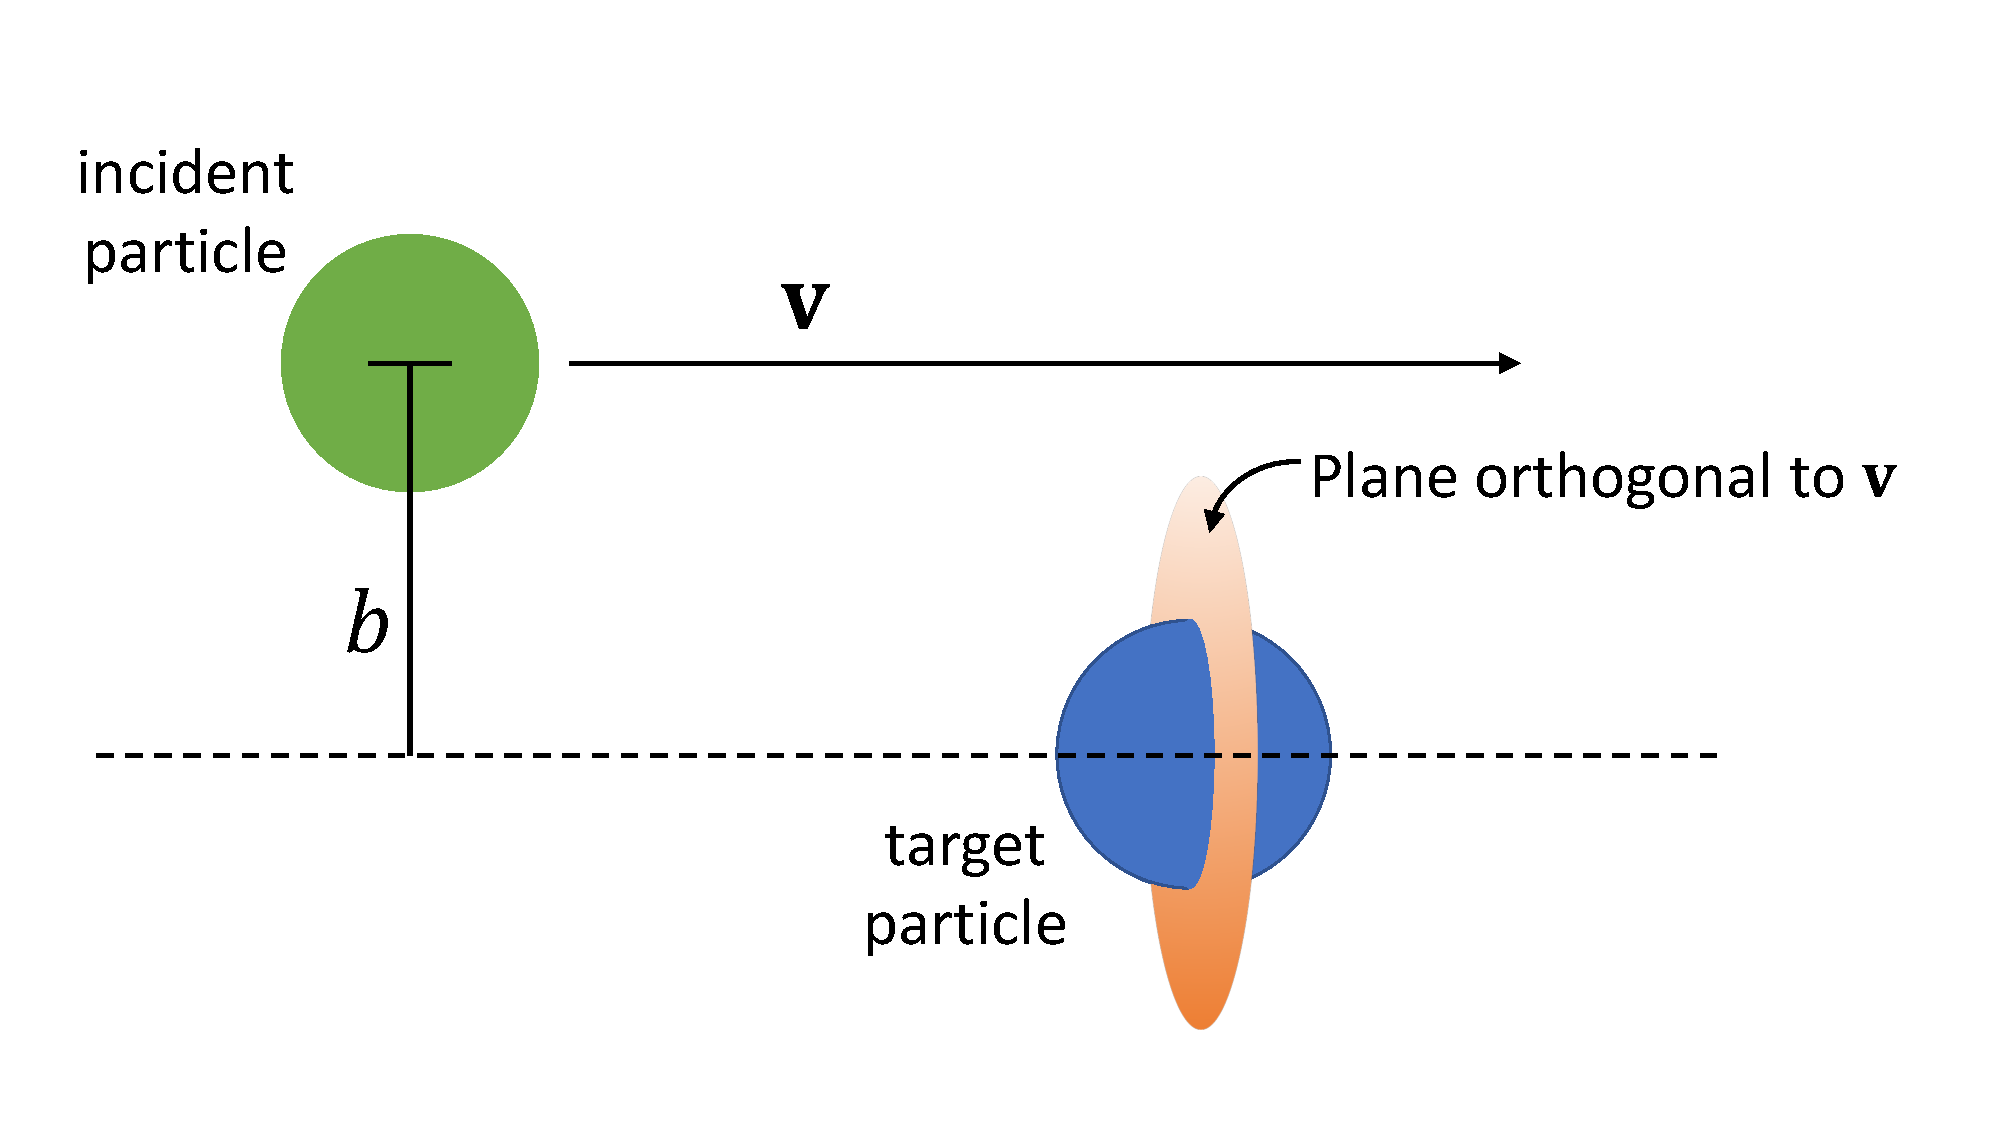
\includegraphics[width=10cm]{../../images/cross_section.pdf}
\caption{Cross section for particle interactions.}
\label{fig:cross_section}
\end{figure}

To quantify the above, the reader is referred to \cref{fig:cross_section}. Imagine an incident particle traveling towards a stationary target particle with an impact parameter $b$ and velocity $\vvec$ (if the target particle is not stationary, then $\vvec = \vvec_2 - \vvec_1$, where $\vvec_1$ is the velocity of the target particle and $\vvec_2$ is the velocity of the incident particle.) As shown in \cref{fig:cross_section}, the impact parameter is the perpendicular offset between the path of the incident particle, and the line parallel to the incident particle velocity that crosses the origin of the target particle (or the origin of the force field of the target particle). To determine the cross section, we ask the following question: for a particle with impact parameter $b$ and velocity magnitude $v = |\vvec|$, does it interact with the target particle? Let's say it does not interact, then the infinitesimal surface located at $b$, i.e.\@ $b db d\phi$ for cylindrical coordinates, does not contribute to the cross section. If it does interact, then $b db d\phi$ does contribute to the cross section. To obtain the total cross section $\sigma = \sigma(v)$, we sum over all infinitesimal areas $b db d\phi$, but account whether a particle at a given $b$ interacts or not with the target particle. This is expressed mathematically as
\begin{equation}
\label{eq:def_cross_section}
    \sigma = \int_0^{2\pi} \int_0^\infty F(v,b) \, b db d\phi.
\end{equation}
In the above $F(v,b) = 1$ if an incident particle with impact parameter $b$ and velocity $v$ interacts with the target particle, and $F(v,b) = 0$ if it does not. However, in reality, $F(v,b)$ is not necessarily binary, and can take other values besides 0 and 1.

An example of $F(v,b)$ is that corresponding to particles that are hard spheres with radius R. For this case, $F(v,b) = H(2R - b)$, where $H$ is the heaviside function. Thus,
\begin{equation}
    \sigma = \int_0^{2\pi} \int_0^\infty H(2R-b) \, b db d\phi = 2\pi \int_0^{2R} b db = \pi (2R)^2,
\end{equation}
as expected.

%-------------------------------------------------------------------------------
\section{Mean free path, collision time, and collision frequency}
%-------------------------------------------------------------------------------
The cross section then defines the mean free path $\lambda_m$, collision time $\tau_m$ and collision frequency $\nu_m$. These are given by
\begin{equation}
    \lambda_m = \frac{1}{n_1 \sigma},
\end{equation}
\begin{equation}
    \tau_m = \frac{\lambda_m}{v} = \frac{1}{n_1 \sigma v},
\end{equation}
and
\begin{equation}
    \nu_{m} = \frac{1}{\tau_m} = n_1 \sigma v.
\end{equation}

%--------------------------------------------------------------------------
\section{Coulomb scattering}
%--------------------------------------------------------------------------
%--------------------------------------------
\subsection{Particle equations}
%--------------------------------------------
Consider two particles, with positions $\rvec_1=\rvec_1(t)$ and $\rvec_2=\rvec_2(t)$, velocities $\vvec_1=\vvec_1(t)$ and $\vvec_2=\vvec_2(t)$, charges $q_1$ and $q_2$, and masses $m_1$ and $m_2$, respectively. Their positions and velocities are governed by the following equations 
\begin{equation}
    \label{eq:particle_1_pos}
    \frac{d \rvec_1}{dt} = \vvec_1,
\end{equation}
\begin{equation}
    \label{eq:particle_2_pos}
    \frac{d \rvec_2}{dt} = \vvec_2,
\end{equation}
\begin{equation}
    \label{eq:particle_1_vel}
    m_1 \frac{d\vvec_1}{dt} = -\frac{q_1 q_2}{4 \pi \epsilon} \frac{\rvec_2 - \rvec_1}{\left | \rvec_2 - \rvec_1 \right |^3},
\end{equation}
\begin{equation}
    \label{eq:particle_2_vel}
    m_2 \frac{d\vvec_2}{dt} = -\frac{q_1 q_2}{4 \pi \epsilon} \frac{\rvec_1 - \rvec_2}{\left | \rvec_1 - \rvec_2 \right |^3}.
\end{equation}
We note that the above system consists of twelve equations for twelve unknowns. We now introduce the center-of-mass position $\Rvec = \Rvec(t)$, the center-of-mass velocity $\Vvec = \Vvec(t)$, the shifted position $\rvec = \rvec(t)$ and the shifted velocity $\vvec = \vvec(t)$ as follows
\begin{equation}
    \Rvec = \frac{m_1 \rvec_1 + m_2 \rvec_2}{m_1 + m_2} \qquad \rvec = \rvec_1 - \rvec_2,
\end{equation}
\begin{equation}
    \Vvec = \frac{m_1 \vvec_1 + m_2 \vvec_2}{m_1 + m_2} \qquad \vvec = \vvec_1 - \vvec_2
\end{equation}
Thus, in terms of these new four variables, the particle equations can be written as
\begin{equation}
    \frac{d \Rvec}{dt} = \Vvec,
\end{equation}
\begin{equation}
    \frac{d \Vvec}{dt} = 0 ,
\end{equation}
\begin{equation}
    \label{eq:particle_pos}
    \frac{d \rvec}{dt} = \vvec,
\end{equation}
\begin{equation}
    \label{eq:particle_vel}
    \frac{d \vvec}{dt} = \frac{q_1 q_2}{4\pi \epsilon_0 m_r} \frac{\rvec}{r^3},
\end{equation}
where the reduced mass $m_r$ is given by
\begin{equation}
    \frac{1}{m_r} = \frac{1}{m_1} + \frac{1}{m_2}.
\end{equation}
The first two equations above give the trivial solution $\Vvec = $ constant and $\Rvec$ = $\Rvec(0) + \Vvec t$. Thus, we have reduced the problem from twelve unknowns to six unknowns, namely $\rvec$ and $\vvec$.

%--------------------------------------------
\subsection{Conservation of energy}
%--------------------------------------------
Dotting \cref{eq:particle_vel} by $\vvec$ gives 
\begin{align}
    \vvec \cdot \frac{d \vvec}{dt} &= \frac{q_1 q_2}{4 \pi \epsilon_0 m_r} \vvec \cdot \frac{\rvec}{r^3} \nonumber \\
    &= \frac{q_1 q_2}{4 \pi \epsilon_0 m_r} \frac{d\rvec}{dt} \cdot \frac{\rvec}{r^3} \nonumber \\
    &= \frac{q_1 q_2}{4 \pi \epsilon_0 m_r} \frac{1}{2} \frac{dr^2}{dt} \frac{1}{r^3} \nonumber \\
    &= \frac{q_1 q_2}{4 \pi \epsilon_0 m_r} \frac{1}{r^2} \frac{dr}{dt} \nonumber \\
    &= -\frac{q_1 q_2}{4 \pi \epsilon_0 m_r} \frac{d}{dt} \left ( \frac{1}{r} \right ).
\end{align} 
For the left hand side above we have
\begin{equation}
    \vvec \cdot \frac{d \vvec}{dt} = \frac{1}{2} \frac{d v^2}{dt},
\end{equation}
and thus we obtain the following expression for conservation of energy
\begin{equation}
    \frac{d}{dt} \left ( \frac{1}{2} m_r v^2 + \frac{q_1 q_2}{4 \pi \epsilon_0} \frac{1}{r} \right ) = 0.
\end{equation}

%--------------------------------------------
\subsection{Conservation of momentum}
%--------------------------------------------
Crossing \cref{eq:particle_vel} by $\rvec$ gives
\begin{equation}
    \rvec \times \frac{d \vvec}{dt} = \frac{q_1 q_2}{4 \pi \epsilon_0 m_r} \frac{\rvec \times \rvec}{r^3} = 0,
\end{equation}
and thus
\begin{equation}
    \frac{d}{dt} \left [ m_r \left ( \rvec \times \vvec \right ) \right ] = 0.
\end{equation}
That is, angular momentum is conserved. A consequence of this is that the vector $\rvec \times \vvec$ is always pointing in the same direction. Thus, if $\rvec(0)$ and $\vvec(0)$ form a plane, then $\rvec(t)$ and $\vvec(t)$ need to reside within that same plane for all times $t$ so that $\rvec(t) \times \vvec(t)$ points in the same direction as $\rvec(0) \times \vvec(0)$. Therefore, the evolution of the position and velocity are confined to a plane and the problem can be reduced from six unknowns to four unknowns. This planar encounter is depicted in \cref{fig:coulomb_scattering}.
\begin{figure}[ht]
    \centering
    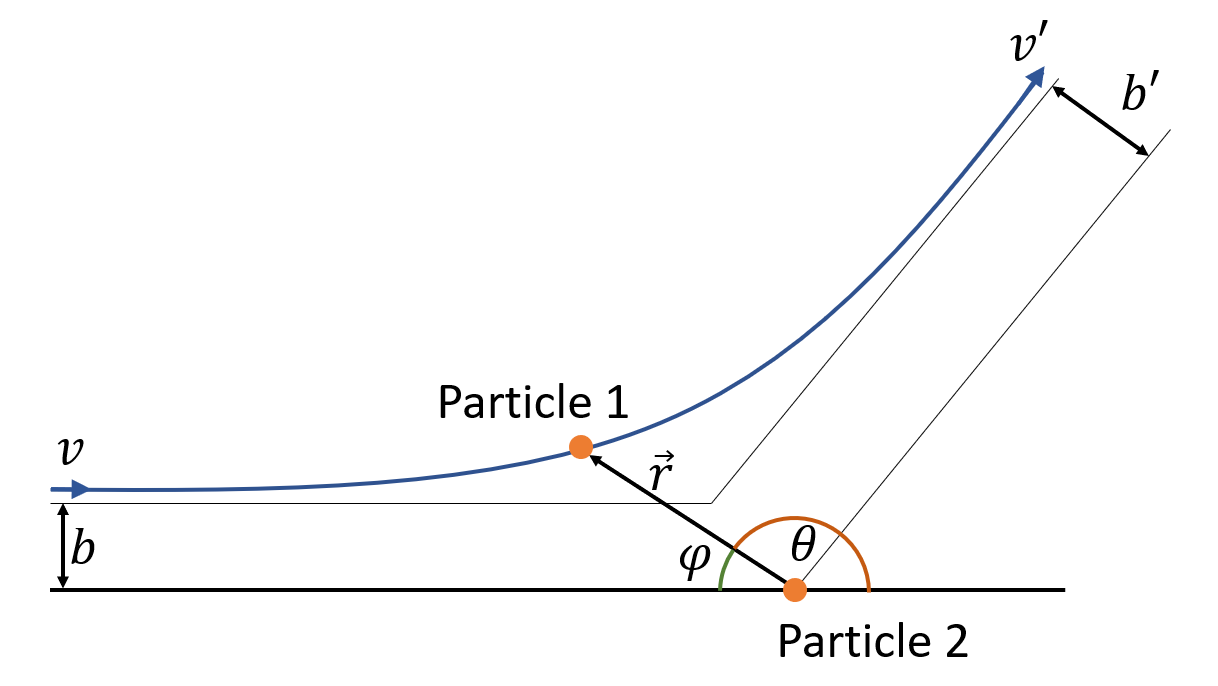
\includegraphics[width=10cm]{../../images/coulomb_scattering.png}
    \caption{Depiction of Coulomb scattering.}
    \label{fig:coulomb_scattering}
    \end{figure}

%--------------------------------------------
\subsection{Polar coordinates}
%--------------------------------------------
\begin{figure}[ht]
    \centering
    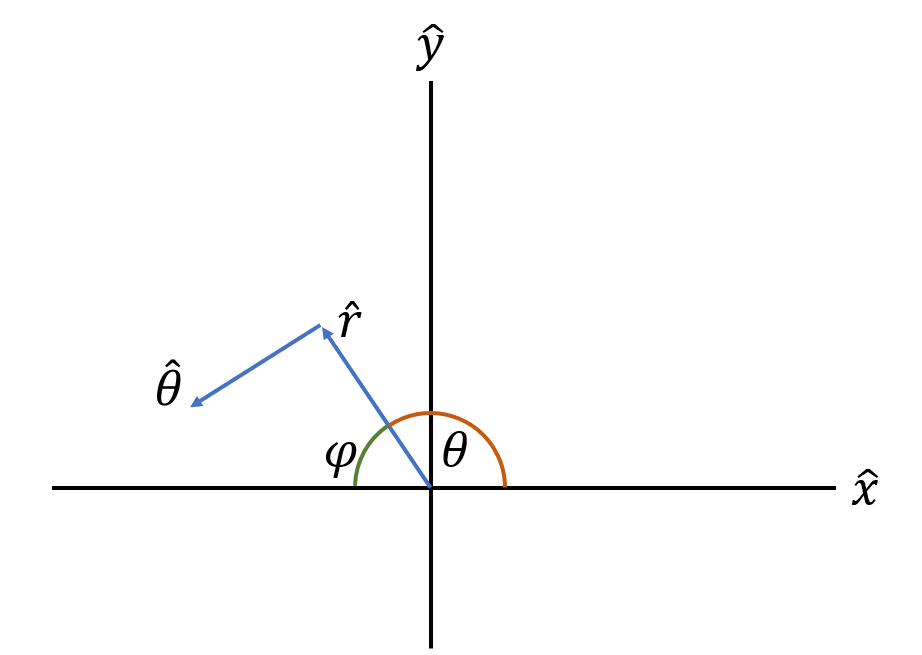
\includegraphics[width=10cm]{../../images/polar_coordinates.png}
    \caption{Polar coordinates in plane of interaction.}
    \label{fig:polar_coordinates}
    \end{figure}

We re-orient the plane of interaction (referred to above) so that it is orthogonal to the $\hat{\zvec}$ direction. Using polar coordinates, as shown in \cref{fig:polar_coordinates}, we get
\begin{equation}
    r_x = r \cos \theta = r \cos ( \pi - \varphi ) = -r \cos \varphi,
\end{equation}
\begin{equation}
    r_y = r \sin \theta = r \sin ( \pi - \varphi ) = r \sin \varphi.
\end{equation}

Also, since $\rvec = r \hat{\rvec}$, we have
\begin{align}
    \vvec = &\frac{d \rvec}{dt} = \frac{dr}{dt} \hat{\rvec} + r \frac{d\hat{\rvec}}{dt} \nonumber \\
    &= \frac{d r}{dt} \hat{\rvec} + r \frac{d\hat{\rvec}}{d\theta} \frac{d\theta}{dt} \nonumber \\
    &= \frac{dr}{dt} \hat{\rvec} + r \frac{d \theta}{dt} \hat{\boldsymbol{\theta}},
\end{align}
and
\begin{align}
    \frac{d \vvec}{dt} &= \frac{d^2r}{dt^2} \hat{\rvec} + \frac{dr}{dt} \frac{d\hat{\rvec}}{dt} + \frac{d}{dt} \left ( r \frac{d\theta}{dt} \right ) \hat{\boldsymbol{\theta}} + r \frac{d \theta}{dt} \frac{d \hat{\boldsymbol{\theta}}}{dt} \nonumber \\
    &= \frac{d^2 r}{dt^2} \hat{\rvec} + \frac{dr}{dt} \frac{d\hat{\rvec}}{d\theta} \frac{d\theta}{dt} + \frac{d}{dt} \left ( r \frac{d\theta}{dt} \right ) \hat{\boldsymbol{\theta}} + r \frac{d \theta}{dt} \frac{d \hat{\boldsymbol{\theta}}}{d\theta} \frac{d \theta}{dt} \nonumber \\
    &= \frac{d^2r}{dt^2} \hat{\rvec} + \frac{dr}{dt} \frac{d\theta}{dt} \hat{\boldsymbol{\theta}} + \frac{d}{dt} \left ( r \frac{d\theta}{dt} \right ) \hat{\boldsymbol{\theta}} - r \left ( \frac{d\theta}{dt} \right ) ^2 \hat{\rvec}.
\end{align}

%--------------------------------------------
\subsection{The force equation}
%--------------------------------------------
The radial component of \cref{eq:particle_vel} thus becomes 
\begin{equation}
    \frac{d^2 r}{dt^2} - r \left ( \frac{d\theta}{dt} \right )^2 = \frac{q_1 q_2}{4 \pi \epsilon_0 m_r} \frac{1}{r^2}.
\end{equation}
Since $\theta = \pi - \varphi$, we have
\begin{equation}
    \label{eq:particle_position_ode}
    \frac{d^2 r}{dt^2} - r \left ( \frac{d\varphi}{dt} \right )^2 = \frac{q_1 q_2}{4 \pi \epsilon_0 m_r} \frac{1}{r^2}.
\end{equation}

%--------------------------------------------
\subsection{The angular momentum equation}
%--------------------------------------------
Using polar coordinates, we obtain
\begin{equation}
    m_r \rvec \times \vvec = m_r r \hat{\rvec} \times \left ( \frac{dr}{dt} \hat{\rvec} + r \frac{d\theta}{dt} \hat{\boldsymbol{\theta}} \right ) = m_r r^2 \frac{d\theta}{dt} \hat{\zvec}
\end{equation}
Since angular momentum $m_r \rvec \times \vvec$ is conserved, we have
\begin{equation}
    \label{eq:particle_cons_angular_polar}
    m_r r^2 \frac{d\varphi}{dt} = L = constant.
\end{equation}
We note here that $L$ is positive since $d\varphi/dt$ is positive. Also, we have 
\begin{equation}
    \label{eq:particle_angular_sign}
    m_r \rvec \times \vvec = -L \hat{\zvec},
\end{equation}
that is, the angular momentum is in the negative $\hat{\zvec}$ direction.

%--------------------------------------------
\subsection{Particle trajectory}
%--------------------------------------------
The goal is to find the radial position of the particle as a function of its angular orientation. That is, we want to find $\tilde{r} = \tilde{r}(\tilde{\varphi})$ such that
\begin{equation}
    \label{eq:particle_position_angle}
    r(t) = \tilde{r}(\varphi(t)).
\end{equation}
To simplify the math, we introduce $\tilde{u} = \tilde{u}(\tilde{\varphi})$ such that $\tilde{u} = 1 / \tilde{r}$. Thus
\begin{equation}
    \frac{d \tilde{u}}{d\tilde{\varphi}} = -\frac{1}{\tilde{r}^2} \frac{d \tilde{r}}{d\tilde{\varphi}},
\end{equation}
or, after re-arranging
\begin{equation}
    \label{eq:rgrad_vs_ugrad}
    \frac{d \tilde{r}}{d\tilde{\varphi}} = -\frac{1}{\tilde{u}^2} \frac{d \tilde{u}}{d\tilde{\varphi}}.
\end{equation}

We now proceed as follows. Taking the derivative of $r$, we get
\begin{align}
    \label{eq:particle_derivation_1}
    \frac{dr}{dt} &= \left ( \frac{d \tilde{r}}{d\tilde{\varphi}} \right )_{\tilde{\varphi} = \varphi(t)} \frac{d \varphi}{dt} &&[\cref{eq:particle_position_angle}] \nonumber \\
    &= \left ( -\frac{1}{\tilde{u}^2} \frac{d\tilde{u}}{d\tilde{\varphi}} \right )_{\tilde{\varphi} = \varphi(t)} \frac{d \varphi}{dt} &&[\cref{eq:rgrad_vs_ugrad}]\nonumber \\ 
    &= \left ( -\frac{1}{\tilde{u}^2} \frac{d\tilde{u}}{d\tilde{\varphi}} \right )_{\tilde{\varphi} = \varphi(t)} \frac{L}{m_r r^2} &&[\cref{eq:particle_cons_angular_polar}] \nonumber \\
    &= \left ( -\frac{1}{\tilde{u}^2} \frac{d\tilde{u}}{d\tilde{\varphi}} \frac{L}{m_r \tilde{r}^2} \right )_{\tilde{\varphi} = \varphi(t)} &&[\cref{eq:particle_position_angle}] \nonumber \\
    &= \left ( - \frac{d\tilde{u}}{d\tilde{\varphi}} \frac{L}{m_r} \right )_{\tilde{\varphi} = \varphi(t)}
\end{align}
Taking the derivative of the above, we get
\begin{align}
    \frac{d}{dt} \frac{dr}{dt} &= \left [ \frac{d}{d\tilde{\varphi}} \left ( - \frac{d\tilde{u}}{d\tilde{\varphi}} \frac{L}{m_r} \right ) \right ]_{\tilde{\varphi} = \varphi(t)} \frac{d \varphi}{dt} \nonumber \\
    &= \left ( - \frac{d^2 \tilde{u}}{d\tilde{\varphi}^2} \frac{L}{m_r} \right )_{\tilde{\varphi} = \varphi(t)} \frac{L}{m_r r^2} && [\cref{eq:particle_cons_angular_polar}] \nonumber \\
    &= \left ( - \frac{d^2 \tilde{u}}{d\tilde{\varphi}^2} \frac{L}{m_r} \frac{L}{m_r \tilde{r}^2} \right )_{\tilde{\varphi} = \varphi(t)} && [\cref{eq:particle_position_angle}] \nonumber \\
    &= \left ( - \frac{d^2 \tilde{u}}{d\tilde{\varphi}^2} \frac{L^2 \tilde{u}^2}{m_r^2} \right )_{\tilde{\varphi} = \varphi(t)}
\end{align}
Plugging the last relation into \cref{eq:particle_position_ode} gives
\begin{equation}
    \left [ - \frac{d^2 \tilde{u}}{d\tilde{\varphi}^2} \frac{L^2 \tilde{u}^2}{m_r^2} - \frac{1}{\tilde{u}} \left ( \frac{L \tilde{u}^2}{m_r} \right )^2 \right ]_{\tilde{\varphi} = \varphi(t)} = \left ( \frac{q_1 q_2}{4 \pi \epsilon_0 m_r} \tilde{u}^2 \right )_{\tilde{\varphi} = \varphi(t)},
\end{equation}
which, upon re-arranging and dropping the $\varphi(t)$ dependance, becomes
\begin{equation}
    \frac{d^2 \tilde{u}}{d \tilde{\varphi}^2} + \tilde{u} = -\frac{q_1 q_2 m_r}{4 \pi \epsilon_0 L^2}
\end{equation}

Using \cref{eq:particle_angular_sign}, we have
\begin{align}
    \label{eq:particle_momentum_impact}
    L &= -m_r ( \rvec \times \vvec )\cdot \hat{\zvec} \nonumber \\
    &= -m_r [\sin(-\theta) r v_0 \hat{\zvec} ] \cdot \hat{\zvec} \nonumber \\
    &= m_r\sin(\theta) r v_0 \nonumber \\
    &= m_r\sin(\pi - \varphi) r v_0 \nonumber \\
    &= m_r\sin\varphi r v_0 \nonumber \\
    &= m_r b v_0.
\end{align}
Thus, we write the evolution equation for $\tilde{u}$ as
\begin{equation}
    \frac{d^2 \tilde{u}}{d \tilde{\varphi}^2} + \tilde{u} = -\frac{q_1 q_2}{4 \pi \epsilon_0 m_r b^2 v_0^2}.
\end{equation}
Introducing the notation
\begin{equation}
    b_{90} = \frac{q_1 q_2}{4 \pi \epsilon_0 m_r v_0^2},
\end{equation}
the evolution equation for $\tilde{u}$ can be simply expressed as
\begin{equation}
    \label{eq:particle_u_equation}
    \frac{d^2 \tilde{u}}{d \tilde{\varphi}^2} + \tilde{u} = -\frac{b_{90}}{b^2}.
\end{equation}

The boundary conditions for \cref{eq:particle_u_equation} are as follows
\begin{equation}
    \label{eq:particle_bc_1}
    \text{as } \varphi(t) \to 0, \quad r(t) \to \infty
\end{equation}
\begin{equation}
    \label{eq:particle_bc_2}
    \text{as } \varphi(t) \to 0, \quad \frac{dr(t)}{dt} \to -v_0
\end{equation}
Given \cref{eq:particle_position_angle}, \cref{eq:particle_bc_1} can only be satisfied if as $\tilde{\varphi} \to 0$, $\tilde{r} \to \infty$. Thus, we also have, as $\tilde{\varphi} \to 0$, $\tilde{u} \to 0$. Similarly, given \cref{eq:particle_derivation_1}, \cref{eq:particle_bc_2} can only be satisfied if as $\tilde{\varphi} \to 0$
\begin{equation}
    \frac{d\tilde{u}}{d\tilde{\varphi}} \frac{L}{m_r} \to v_0.
\end{equation}
Using \cref{eq:particle_momentum_impact} we rewrite the above as 
\begin{equation}
    \frac{d\tilde{u}}{d\tilde{\varphi}} \to \frac{1}{b}.
\end{equation}

The general solution to \cref{eq:particle_u_equation} is 
\begin{equation}
    \tilde{u} = A \cos \tilde{\varphi} + B \sin \tilde{\varphi} - \frac{b_{90}}{b^2}.
\end{equation}
Applying the boundary conditions, we get
\begin{equation}
    \tilde{u} = \frac{b_{90}}{b^2} \cos \tilde{\varphi} + \frac{1}{b} \sin \tilde{\varphi} - \frac{b_{90}}{b^2},
\end{equation}
which we finally re-write as
\begin{equation}
    \frac{1}{\tilde{r}} = \frac{1}{b} \sin \tilde{\varphi} + \frac{b_{90}}{b^2} \left ( \cos \tilde{\varphi} - 1 \right ).
\end{equation}

%###############################################################################
%
%
\part{Kinetic description}
%
%
%###############################################################################
%-------------------------------------------------------------------------------
\chapter{Governing equations}
%-------------------------------------------------------------------------------

We denote the distribution function for a species $\alpha$ as $f_\alpha = f_\alpha(\rvec, \vvec, t)$, where $\rvec$ and $\vvec$ are the sample space variables for position and velocity. Note that the distribution function is appropriately normalized such that
\begin{equation}
\int f_\alpha \, d\rvec d\vvec = N_\alpha,
\end{equation}
where $N_\alpha$ is the total number of particles corresponding to species $\alpha$. 

The dynamics of a plasma can be characterized by the Boltzmann evolution equation for the distribution along with Maxwell's equations
\begin{equation}
\label{eq:kinetic_equation}
\frac{\partial f_\alpha}{\partial t} + \vvec \cdot \nabla f_\alpha + \frac{Z_\alpha e}{m_\alpha} ( \Evec + \vvec \times \Bvec ) \cdot \nabla_v f_\alpha = C_\alpha + S_\alpha
\end{equation}
\begin{equation}
\label{eq:maxwell_3}
\nabla \cdot \Evec = \frac{\rho_e}{\epsilon_0} 
\end{equation}
\begin{equation}
\label{eq:maxwell_4}
\nabla \cdot \Bvec = 0
\end{equation}
\begin{equation}
\label{eq:maxwell_1}
\nabla \times \Evec = -\frac{ \partial \Bvec}{\partial t}
\end{equation}
\begin{equation}
\label{eq:maxwell_2}
\nabla \times \Bvec = \mu_0 \Jvec + \mu_0 \epsilon_0 \frac{\partial \Evec}{\partial t}
\end{equation}
\begin{equation}
\Jvec = \sum_\alpha Z_\alpha e \int \vvec f_\alpha \, d\vvec
\end{equation}
\begin{equation}
\rho_e = \sum_\alpha Z_\alpha e \int f_\alpha \, d\vvec.
\end{equation}
In the above, 
\begin{itemize}
\item $m_\alpha$ is the species mass
\item $e$ is the charge
\item $Z_\alpha$ the charge number
\item $\Jvec = \Jvec(\rvec,t)$ the charge current
\item $\rho_e = \rho_e(\rvec,t)$ the charge density
\item $\Evec = \Evec(\rvec,t)$ the electric field
\item $\Bvec = \Bvec(\rvec,t)$ the magnetic field.
\end{itemize}
The terms $C_\alpha$ and $S_\alpha$ represent collision and source terms.

If we express the collision term in the usual way, that is $C_\alpha = \sum_\beta C_{\alpha \beta}$, then we can make the following statements:
\begin{enumerate}
\item Conservation of particles:
\begin{equation}
\int C_{\alpha \alpha} \, d\vvec = 0 \quad \forall \alpha \qquad \qquad
\int C_{\alpha \beta} \,d\vvec = 0 \quad \forall \alpha, \beta | \beta \ne \alpha.
\end{equation}

\item Conservation of momentum:
\begin{equation}
\int m_\alpha \vvec C_{\alpha \alpha} \, d\vvec = 0 \quad \forall \alpha \qquad \qquad \sum_\alpha \sum_{\beta, \beta \ne \alpha} \int m_\alpha \vvec C_{\alpha \beta} d\vvec = 0.
\end{equation}

\item Conservation of energy:
\begin{equation}
\int \frac{1}{2} m_\alpha v^2 C_{\alpha \alpha} \, d\vvec = 0 \quad \forall \alpha \qquad \qquad \sum_\alpha \sum_{\beta, \beta \ne \alpha} \int \frac{1}{2} m_\alpha v^2 C_{\alpha \beta} \, d\vvec = 0.
\end{equation}

\end{enumerate}

%-------------------------------------------------------------------------------
\section{Fluid equations}
%-------------------------------------------------------------------------------
We now define the particle density $n_\alpha = n_\alpha(\rvec,t)$, the fluid velocity $\uvec_\alpha = \uvec_\alpha(\rvec,t)$ and the fluid energy per unit mass $E_\alpha = E_\alpha(\rvec,t)$ as follows
\begin{align}
n_\alpha &= \int f_\alpha \, d\vvec \\
\uvec_\alpha &= \frac{1}{n_\alpha} \int \vvec f_\alpha \, d\vvec \\
E_\alpha &= \frac{1}{n_\alpha} \int \frac{1}{2} v^2 f_\alpha \, d\vvec.
\end{align}
Their evolution equations are obtained by taking the appropriate moments of the Boltzmann plasma equation. Before doing so, we re-write the Boltzmann equation as
\begin{equation}
\label{eq:boltz_mod}
\frac{\partial f_\alpha}{\partial t} + \nabla \cdot (\vvec f_\alpha) + \nabla_v \cdot \left [ \frac{Z_\alpha e}{m_\alpha} ( \Evec + \vvec \times \Bvec ) f_\alpha \right ] = C_\alpha + S_\alpha
\end{equation}

%--------------------------------------------
\subsection{Mass}
%--------------------------------------------
Integrating \cref{eq:boltz_mod} over all $\vvec$ we obtain
%\begin{empheq}[box=\widefbox]{equation}
\begin{equation}
\frac{\partial n_\alpha}{\partial t} + \nabla \cdot \left ( n_\alpha \uvec_\alpha \right ) = \hat{S}_\alpha
\end{equation}
%\end{empheq}
where 
\begin{equation}
\hat{S}_\alpha = \int S_\alpha \, d\vvec
\end{equation}
is an external source of mass.

%--------------------------------------------
\subsection{Momentum}
%--------------------------------------------
Multiplying \cref{eq:boltz_mod} by $\vvec$ and then integrating over all $\vvec$ leads to
\begin{multline}
\label{eq:mom_derv_1}
\frac{\partial n_\alpha \uvec_\alpha}{\partial t} + \nabla \cdot \left ( \int \vvec \vvec f_\alpha \, d\vvec \right) + \int \nabla_v \cdot \left [ \vvec \frac{Z_\alpha e}{m_\alpha} ( \Evec + \vvec \times \Bvec ) f_\alpha \right ] - \nabla_v \vvec \cdot \left [ \frac{Z_\alpha e}{m_\alpha} ( \Evec + \vvec \times \Bvec ) f_\alpha \right ] \, d\vvec =\\
\sum_{\beta, \beta \ne \alpha} \int \vvec C_{\alpha \beta} \, d\vvec + \int \vvec S_\alpha \, d\vvec.
\end{multline}
We note that the third term in \cref{eq:mom_derv_1} is zero since we are integrating over all space, and that $\nabla_v \vvec$ is the identity matrix. We thus have
\begin{multline}
\label{eq:mom_derv_2}
\frac{\partial n_\alpha \uvec_\alpha}{\partial t} + \nabla \cdot \left ( \int \vvec \vvec f_\alpha \, d\vvec \right) - \frac{Z_\alpha e n_\alpha}{m_\alpha} ( \Evec + \uvec_\alpha \times \Bvec ) =\\
\sum_{\beta, \beta \ne \alpha} \int \vvec C_{\alpha \beta} \, d\vvec + \int \vvec S_\alpha \, d\vvec.
\end{multline}

To proceed, we decompose $\vvec$ into a mean and a fluctuation, that is, $\vvec = \uvec_\alpha + \wvec_\alpha$. Using this decomposition 
\begin{equation}
\label{eq:identity_vv}
\int \vvec \vvec f_\alpha \, d\vvec = \int ( \uvec_\alpha \uvec_\alpha + 2 \uvec_\alpha \wvec_\alpha + \wvec_\alpha \wvec_\alpha) f_\alpha \, d\vvec = n_\alpha \uvec_\alpha \uvec_\alpha + \int \wvec_\alpha \wvec_\alpha f_\alpha \, d\vvec.
\end{equation}
Thus, \cref{eq:mom_derv_2} becomes
\begin{multline}
\label{eq:mom_derv_3}
\frac{\partial n_\alpha \uvec_\alpha}{\partial t} + \nabla \cdot \left ( n_\alpha \uvec_\alpha \uvec_\alpha \right) - \frac{Z_\alpha e n_\alpha}{m_\alpha} ( \Evec + \uvec_\alpha \times \Bvec ) = -\nabla \cdot \int \wvec_\alpha \wvec_\alpha f_\alpha d\vvec + \\
\sum_{\beta, \beta \ne \alpha} \int \vvec C_{\alpha \beta} \, d\vvec + \int \vvec S_\alpha \, d\vvec.
\end{multline}
Conservation of particles is used to modify the collisional term to thus obtain
\begin{multline}
\label{eq:mom_derv_4}
\frac{\partial n_\alpha \uvec_\alpha}{\partial t} + \nabla \cdot \left ( n_\alpha \uvec_\alpha \uvec_\alpha \right) - \frac{Z_\alpha e n_\alpha}{m_\alpha} ( \Evec + \uvec_\alpha \times \Bvec ) = -\nabla \cdot \int \wvec_\alpha \wvec_\alpha f_\alpha d\vvec + \\
\sum_{\beta, \beta \ne \alpha} \int \wvec_\alpha C_{\alpha \beta} \, d\vvec + \int \vvec S_\alpha \, d\vvec.
\end{multline}

Multiplying by mass leads to the following equation
%\begin{empheq}[box=\widefbox]{equation}
\begin{equation}
\label{eq:mom_derv_5}
\frac{\partial m_\alpha n_\alpha \uvec_\alpha}{\partial t} + \nabla \cdot \left ( m_\alpha n_\alpha \uvec_\alpha \uvec_\alpha \right) - Z_\alpha e n_\alpha ( \Evec + \uvec_\alpha \times \Bvec ) = \nabla \cdot \boldsymbol{\sigma}_\alpha + \Rvec_\alpha + \hat{\Mvec}_\alpha,
\end{equation}
%\end{empheq}
where the stress tensor is
\begin{equation}
\boldsymbol{\sigma}_\alpha = -\int m_\alpha \wvec_\alpha \wvec_\alpha f_\alpha \, d\vvec,
\end{equation}
the momentum transferred between unlike particles due to friction of collisions is
\begin{equation}
\Rvec_\alpha = \sum_{\beta, \beta \ne \alpha} \int m_\alpha \wvec_\alpha C_{\alpha \beta} \, d\vvec,
\end{equation}
and the external source of momentum is
\begin{equation}
\hat{\Mvec}_\alpha = \int m_\alpha \vvec S_\alpha \, d\vvec.
\end{equation}
 

The stress tensor is typically decomposed into isotropic $p_\alpha$ and anisotropic (shear) $\tvec_\alpha$ tensors as follows
\begin{equation}
\boldsymbol{\sigma}_\alpha = - p_\alpha \Ivec + \tvec_\alpha,
\end{equation}
where $P_\alpha$ is given by
\begin{equation}
p_\alpha = \frac{1}{3} \int m_\alpha (\wvec_\alpha \cdot \wvec_\alpha) f_\alpha d\vvec.
\end{equation}
Thus, conservation of momentum becomes
\begin{equation}
\label{eq:mom_derv_6}
\frac{\partial m_\alpha n_\alpha \uvec_\alpha}{\partial t} + \nabla \cdot \left ( m_\alpha n_\alpha \uvec_\alpha \uvec_\alpha \right) - Z_\alpha e n_\alpha ( \Evec + \uvec_\alpha \times \Bvec ) = - \nabla p_\alpha + \nabla \cdot \tvec_\alpha + \Rvec_\alpha + \hat{\Mvec}_\alpha.
\end{equation}

%--------------------------------------------
\subsection{Energy}
%--------------------------------------------
Multiplying \cref{eq:boltz_mod} by $\frac{1}{2} v^2$ and then integrating over all $\vvec$ leads to
\begin{multline}
\label{eq:energy_derv_1}
\frac{\partial n_\alpha E_\alpha}{\partial t} + \nabla \cdot \left [ \int \frac{1}{2} (\vvec \cdot \vvec) \vvec f_\alpha \, d\vvec \right ] + \int \nabla_v \cdot \left [ \frac{1}{2} (\vvec \cdot \vvec) \frac{Z_\alpha e}{m_\alpha} ( \Evec + \vvec \times \Bvec ) f_\alpha \right ] \\
- \nabla_v \left [ \frac{1}{2} (\vvec \cdot \vvec) \right ] \cdot \left [ \frac{Z_\alpha e}{m_\alpha} ( \Evec + \vvec \times \Bvec ) f_\alpha \right ] \, d\vvec = \sum_{\beta, \beta \ne \alpha} \int \frac{1}{2} (\vvec \cdot \vvec) C_{\alpha \beta} \, d\vvec + \int \frac{1}{2} (\vvec \cdot \vvec) S_\alpha \, d\vvec.
\end{multline}
We note that the third term above is zero since we are integrating over all space, and that $\nabla_v [ 1/2 (\vvec \cdot \vvec ) ] = \vvec$. Thus, we have
\begin{multline}
\label{eq:energy_derv_2}
\frac{\partial n_\alpha E_\alpha}{\partial t} + \nabla \cdot \left [ \int \frac{1}{2} (\vvec \cdot \vvec) \vvec f_\alpha \, d\vvec \right ] - \frac{Z_\alpha e n_\alpha}{m_\alpha} \Evec \cdot \uvec_\alpha =\\
\sum_{\beta, \beta \ne \alpha} \int \frac{1}{2} (\vvec \cdot \vvec) C_{\alpha \beta} \, d\vvec + \int \frac{1}{2} (\vvec \cdot \vvec) S_\alpha \, d\vvec.
\end{multline}

To proceed with the derivation we first note that
\begin{multline}
\int \frac{1}{2} (\vvec \cdot \vvec) \vvec f_\alpha \, d\vvec = \int \frac{1}{2} (\vvec \cdot \vvec) (\uvec_\alpha + \wvec_\alpha) f_\alpha \, d\vvec = n_\alpha E_\alpha \uvec_\alpha + \int \frac{1}{2} (\vvec \cdot \vvec ) \wvec_\alpha f_\alpha \, d\vvec
\end{multline}
The last term on the right-hand side above can be re-written as
\begin{align}
\int \frac{1}{2} ( \vvec \cdot \vvec ) \wvec_\alpha f_\alpha \, d\vvec &= \int \frac{1}{2} ( \uvec_\alpha \cdot \uvec_\alpha + 2\uvec_\alpha \cdot \wvec_\alpha + \wvec_\alpha \cdot \wvec_\alpha ) \wvec_\alpha f_\alpha \, d\vvec \\
& =  \uvec_\alpha \cdot \int \wvec_\alpha \wvec_\alpha f_\alpha \, d\vvec + \int \frac{1}{2} ( \wvec_\alpha \cdot \wvec_\alpha ) \wvec_\alpha f_\alpha \, d\vvec.
\end{align}
Using the expressions above, \cref{eq:energy_derv_2} becomes
\begin{multline}
\label{eq:energy_derv_3}
\frac{\partial n_\alpha E_\alpha}{\partial t} + \nabla \cdot (n_\alpha E_\alpha \uvec_\alpha ) - \frac{Z_\alpha e n_\alpha}{m_\alpha} \Evec \cdot \uvec_\alpha =  - \nabla \cdot \left ( \uvec_\alpha \cdot \int \wvec_\alpha \wvec_\alpha f_\alpha \, d\vvec \right ) - \nabla \cdot \int \frac{1}{2} ( \wvec_\alpha \cdot \wvec_\alpha ) \wvec_\alpha f_\alpha \, d\vvec\\
+ \sum_{\beta, \beta \ne \alpha} \int \frac{1}{2} (\vvec \cdot \vvec) C_{\alpha \beta} \, d\vvec + \int \frac{1}{2} (\vvec \cdot \vvec) S_\alpha \, d\vvec.
\end{multline}
Conservation of particles is used to modify the collisional term to thus obtain
\begin{multline}
\label{eq:energy_derv_4}
\frac{\partial n_\alpha E_\alpha}{\partial t} + \nabla \cdot (n_\alpha E_\alpha \uvec_\alpha ) - \frac{Z_\alpha e n_\alpha}{m_\alpha} \Evec \cdot \uvec_\alpha = - \nabla \cdot \left ( \uvec_\alpha \cdot \int \wvec_\alpha \wvec_\alpha f_\alpha \, d\vvec  \right ) - \nabla \cdot \int \frac{1}{2} ( \wvec_\alpha \cdot \wvec_\alpha ) \wvec_\alpha f_\alpha \, d\vvec \\
+ \uvec_\alpha \cdot \sum_{\beta,\beta \ne \alpha} \int \wvec_\alpha C_{\alpha \beta} \, d\vvec + \sum_{\beta, \beta \ne \alpha} \int \frac{1}{2} (\wvec_\alpha \cdot \wvec_\alpha) C_{\alpha \beta} \, d\vvec + \int \frac{1}{2} (\vvec \cdot \vvec) S_\alpha \, d\vvec.
\end{multline}

Multiplying by mass leads to the following equation
%\begin{empheq}[box=\widefbox]{multline}
\begin{multline}
\label{eq:energy_derv_5}
\frac{\partial m_\alpha n_\alpha E_\alpha}{\partial t} + \nabla \cdot (m_\alpha n_\alpha E_\alpha \uvec_\alpha ) - Z_\alpha e n_\alpha \Evec \cdot \uvec_\alpha = \nabla \cdot ( \uvec_\alpha \cdot \boldsymbol{\sigma}_\alpha ) - \nabla \cdot \qvec_\alpha \\
+ \uvec_\alpha \cdot \Rvec_\alpha + Q_{\alpha} + \hat{Q}_\alpha, 
\end{multline}
%\end{empheq}
where heat flux due to random motion is
\begin{equation}
\qvec_\alpha = \int \frac{1}{2} m_\alpha (\wvec_\alpha \cdot \wvec_\alpha ) \wvec_\alpha f_\alpha \, d\vvec,
\end{equation}
the heat generated and transferred between unlike particles due to collisional dissipation is 
\begin{equation}
Q_{\alpha} = \sum_{\beta,\beta \ne \alpha} \int \frac{1}{2} m_\alpha (\wvec_\alpha \cdot \wvec_\alpha) C_{\alpha \beta} \, d\vvec,
\end{equation}
and the external source of energy is
\begin{equation}
\hat{Q}_\alpha = \int \frac{1}{2} m_\alpha (\vvec \cdot \vvec) S_\alpha \, d\vvec.
\end{equation}

Using the decomposition for the stress tensor, the conservation of energy equation becomes
\begin{multline}
\label{eq:energy_derv_6}
\frac{\partial m_\alpha n_\alpha E_\alpha}{\partial t} + \nabla \cdot (m_\alpha n_\alpha E_\alpha \uvec_\alpha + p_\alpha \uvec_\alpha ) - Z_\alpha e n_\alpha \Evec \cdot \uvec_\alpha = \nabla \cdot ( \uvec_\alpha \cdot \tvec_\alpha ) - \nabla \cdot \qvec_\alpha \\
+ \uvec_\alpha \cdot \Rvec_\alpha + Q_{\alpha} + \hat{Q}_\alpha, 
\end{multline}
We also note that the energy $m_\alpha n_\alpha E_\alpha$ can be decomposed into internal and kinetic energies. Using the trace of the decomposition shown in \cref{eq:identity_vv} one obtains
\begin{align}
m_\alpha n_\alpha E_\alpha & = \int \frac{1}{2} m_\alpha (\vvec \cdot \vvec) f_\alpha \, d\vvec \nonumber \\
& = \int \frac{1}{2} m_\alpha (\wvec_\alpha \cdot \wvec_\alpha) f_\alpha \, d\vvec + \frac{1}{2} m_\alpha n_\alpha (\uvec_\alpha \cdot \uvec_\alpha) \nonumber \\
& = \frac{3}{2} P_\alpha + \frac{1}{2} m_\alpha n_\alpha (\uvec_\alpha \cdot \uvec_\alpha) \nonumber \\
& = \frac{3}{2} P_\alpha + m_\alpha n_\alpha K_\alpha.
\end{align}
where $K_\alpha = \frac{1}{2} \uvec_\alpha \cdot \uvec_\alpha$ is the kinetic energy of species $\alpha$.

%--------------------------------------------
\subsection{Kinetic and Internal Energies}
%--------------------------------------------
The equation for the kinetic energy is obtained by dotting \cref{eq:mom_derv_6} with $\uvec_\alpha$. For this, we first show that
\begin{align}
    \uvec_\alpha \cdot &\left [ \frac{\partial m_\alpha n_\alpha \uvec_\alpha}{\partial t} + \nabla \cdot \left ( m_\alpha n_\alpha \uvec_\alpha \uvec_\alpha \right) \right ] \\
    & =\uvec_\alpha \cdot \left \{ \left [ \frac{\partial m_\alpha n_\alpha }{\partial t} + \nabla \cdot \left ( m_\alpha n_\alpha \uvec_\alpha \right) \right] \uvec_\alpha  + m_\alpha n_\alpha \left ( \frac{\partial \uvec_\alpha}{\partial t} + \uvec_\alpha \cdot \nabla \uvec_\alpha \right ) \right \}\\
    & =\uvec_\alpha \cdot \left [ m_\alpha \hat{S}_\alpha \uvec_\alpha  + m_\alpha n_\alpha \left ( \frac{\partial \uvec_\alpha}{\partial t} + \uvec_\alpha \cdot \nabla \uvec_\alpha \right ) \right ] \\
    & =2m_\alpha \hat{S}_\alpha K_\alpha + m_\alpha n_\alpha \left ( \frac{\partial K_\alpha}{\partial t} + \uvec_\alpha \cdot \nabla K_\alpha \right) \\
    & =m_\alpha \hat{S}_\alpha K_\alpha + \left [ \frac{\partial m_\alpha n_\alpha}{\partial t} + \nabla \cdot \left (m_\alpha n_\alpha \uvec_\alpha \right ) \right] K_\alpha + m_\alpha n_\alpha \left ( \frac{\partial K_\alpha}{\partial t} + \uvec_\alpha \cdot \nabla K_\alpha \right) \\
    & =m_\alpha \hat{S}_\alpha K_\alpha + \frac{\partial m_\alpha n_\alpha K_\alpha}{\partial t} + \nabla \cdot ( m_\alpha n_\alpha K \uvec_\alpha ).
\end{align}
Thus, the equation for the turbulent kinetic energy is
\begin{multline}
\frac{\partial m_\alpha n_\alpha K_\alpha}{\partial t} + \nabla \cdot ( m_\alpha n_\alpha K \uvec_\alpha ) - Z_\alpha e n_\alpha \Evec \cdot \uvec_\alpha =\\
-\nabla \cdot ( \uvec_\alpha p_\alpha ) + \nabla \cdot (\uvec_\alpha \cdot \tvec_\alpha ) + p_\alpha \nabla \cdot \uvec_\alpha - \tvec_\alpha : \nabla \uvec_\alpha + \uvec_\alpha \cdot \Rvec_\alpha + \uvec_\alpha \cdot \hat{\Mvec}_\alpha - m_\alpha K_\alpha \hat{S}_\alpha .
\end{multline}
Subtracting the above equation from \cref{eq:energy_derv_6} leads to 
\begin{equation}
\frac{\partial}{\partial t} \left ( \frac{3}{2} p_\alpha \right ) + \nabla \cdot \left ( \frac{3}{2} p_\alpha \uvec_\alpha \right ) = -p_\alpha \nabla \cdot \uvec_\alpha + \tvec_\alpha : \nabla \uvec_\alpha - \nabla \cdot \qvec_\alpha + Q_{\alpha} + \hat{Q}_\alpha - \uvec_\alpha \cdot \hat{\Mvec}_\alpha + m_\alpha K_\alpha \hat{S}_\alpha .
\end{equation}

%--------------------------------------------
\subsection{Summary}
%--------------------------------------------
To summarize, we have,
\begin{itemize}
    \item Particle density
\begin{equation}
\label{eq:cons_mass}
    \frac{\partial n_\alpha}{\partial t} + \nabla \cdot \left ( n_\alpha \uvec_\alpha \right ) = \hat{S}_\alpha,
\end{equation}

    \item Momentum
\begin{equation}
\label{eq:cons_mom}
    \frac{\partial m_\alpha n_\alpha \uvec_\alpha}{\partial t} + \nabla \cdot \left ( m_\alpha n_\alpha \uvec_\alpha \uvec_\alpha \right) - Z_\alpha e n_\alpha ( \Evec + \uvec_\alpha \times \Bvec ) = - \nabla p_\alpha + \nabla \cdot \tvec_\alpha + \Rvec_\alpha + \hat{\Mvec}_\alpha,
\end{equation}

    \item Total Energy
\begin{multline}
\label{eq:cons_te}
\frac{\partial m_\alpha n_\alpha E_\alpha}{\partial t} + \nabla \cdot (m_\alpha n_\alpha E_\alpha \uvec_\alpha + p_\alpha \uvec_\alpha ) - Z_\alpha e n_\alpha \Evec \cdot \uvec_\alpha = \nabla \cdot ( \uvec_\alpha \cdot \tvec_\alpha ) - \nabla \cdot \qvec_\alpha \\
+ \uvec_\alpha \cdot \Rvec_\alpha + Q_{\alpha} + \hat{Q}_\alpha, 
\end{multline}
    
    \item Kinetic Energy
\begin{multline}
\label{eq:cons_ke}
\frac{\partial m_\alpha n_\alpha K_\alpha}{\partial t} + \nabla \cdot ( m_\alpha n_\alpha K \uvec_\alpha ) - Z_\alpha e n_\alpha \Evec \cdot \uvec_\alpha =\\
-\nabla \cdot ( \uvec_\alpha p_\alpha ) + \nabla \cdot (\uvec_\alpha \cdot \tvec_\alpha ) + p_\alpha \nabla \cdot \uvec_\alpha - \tvec_\alpha : \nabla \uvec_\alpha + \uvec_\alpha \cdot \Rvec_\alpha + \uvec_\alpha \cdot \hat{\Mvec}_\alpha - m_\alpha K_\alpha \hat{S}_\alpha .
\end{multline}    
    
    \item Internal Energy
\begin{equation}
\label{eq:cons_ie}
    \frac{\partial}{\partial t} \left ( \frac{3}{2} p_\alpha \right ) + \nabla \cdot \left ( \frac{3}{2} p_\alpha \uvec_\alpha \right ) = -p_\alpha \nabla \cdot \uvec_\alpha + \tvec_\alpha : \nabla \uvec_\alpha - \nabla \cdot \qvec_\alpha + Q_{\alpha} + \hat{Q}_\alpha - \uvec_\alpha \cdot \hat{\Mvec}_\alpha + m_\alpha K_\alpha \hat{S}_\alpha .  
\end{equation}

\end{itemize}

%-------------------------------------------------------------------------------
\chapter{Transport coefficients}
%-------------------------------------------------------------------------------
Collison integral

\begin{equation}
    \Omega_{\alpha \beta}^{(lk)} = \sqrt{ \frac{k_B T}{2 \pi M_{\alpha \beta}} } \int_0^\infty e^{-g^2} g^{2k+3} \phi_{\alpha \beta}^{(l)} \, dg.
\end{equation}
In the above $M_{\alpha \beta}$ is the reduced mass, given by
\begin{equation}
    M_{\alpha \beta} = \frac{M_\alpha M_\beta}{M_\alpha + M_\beta},
\end{equation}
and $\phi^{(l)}_{\alpha \beta}$ is the collision cross section for a given velocity, and is computed as
\begin{equation}
    \phi_{\alpha \beta}^{(l)} = 2 \pi \int_0^\infty \left ( 1 - \cos^l \chi_{\alpha \beta} \right ) b \, db.
\end{equation}
The scattering angle $\chi_{\alpha \beta}$ is given by
\begin{equation}
    \chi_{\alpha \beta} = \pi - 2 \int_{r_{\alpha \beta}^{\text{min}}}^\infty \frac{b}{r^2 \left [ 1 - \frac{b^2}{r^2} - \frac{V_{\alpha \beta (r)}}{g^2 k_B T} \right ]^{1/2} } \, dr.
\end{equation}

For a Coulombic interaction between ions, we can define the natural scale fore the cross-sectional area as
\begin{equation}
    \phi^{(0)}_{\alpha \beta} = \frac{ \pi \left (Z_\alpha Z_\beta e^2 \right)^2}{ \left(2 k_B T\right)^2}.
\end{equation}
Given this definition, we express the collision integral as
\begin{equation}
    \Omega_{\alpha \beta} = \sqrt{ \frac{\pi }{M_{\alpha \beta}}} \frac{( Z_\alpha Z_\beta e^2)^2 }{(2 k_B T )^{3/2}} \mathcal{F}^{lk}_{\alpha \beta},
\end{equation}
where
\begin{equation}
    \mathcal{F}^{(lk)}_{\alpha \beta} = \frac{1}{2 \phi_0} \int_0^\infty e^{-g^2} g^{2k+3} \phi_{\alpha \beta}^{(l)} \, dg
\end{equation}
We note that $\mathcal{F}^{(lk)}_{\alpha \beta} = 4 \mathcal{K}_{lk}(g_{\alpha \beta})$, where $\mathcal{K}_{lk}(g_{\alpha \beta})$ is the notation from the Stanton-Murillo paper.

%%-------------------------------------------------------------------------------
%\section{Chapman-Enskog Method}
%%-------------------------------------------------------------------------------
%Equations \eqref{eq:cons_mass}, \eqref{eq:mom_derv_5}, and \eqref{eq:energy_derv_5} have many unclosed terms. To %simplify matters a bit, we'll look at the case where there is only one species, there is no external source %$S_\alpha$, and there is no external electromagnetic force. In that case, the fluid equations look as follows
%\begin{equation}
%\label{eq:cons_mass_simple}
%\frac{\partial n}{\partial t} + \nabla \cdot \left ( n \uvec \right ) = 0,
%\end{equation}
%\begin{equation}
%\label{eq:cons_mom_simple}
%\frac{\partial m n \uvec}{\partial t} + \nabla \cdot \left ( m n \uvec \uvec \right) = \nabla \cdot %\boldsymbol{\sigma},
%\end{equation}
%\begin{equation}
%\label{eq:cons_ene_simple}
%\frac{\partial m n E}{\partial t} + \nabla \cdot (m n E \uvec ) = - \nabla \cdot \qvec + \nabla \cdot ( %\boldsymbol{\sigma} \cdot \uvec ).
%\end{equation}
%For the above, the unclosed terms are $\sigma$ and $\qvec$. An approach to obtain approximations to such values is %called the Chapman-Enskog method.

%The kinetic equation for the distribution function, in this case where there is one species and no external sources %and forces, is given by
%\begin{equation}
%    \frac{\partial f}{\partial t} + \vvec \cdot \nabla f = C.
%\end{equation}

%###############################################################################
%
%
\part{Fluid description}
%
%
%###############################################################################

%-------------------------------------------------------------------------------
\chapter{Magnetohydrodynamics}
%-------------------------------------------------------------------------------
%--------------------------------------------
\section{Two-fluid equations}
%--------------------------------------------
The starting point are the multi-fluid conservation laws \cref{eq:cons_mass,eq:cons_mom,eq:cons_ie} and the Maxwell equations \cref{eq:maxwell_1,eq:maxwell_2,eq:maxwell_3,eq:maxwell_4}. We assume there are two species: electrons and singly-charged ions. Additionally, we assume no sources. Thus, the starting governing equations are
\begin{equation}
\label{eq:twof_ni}
    \frac{\partial n_i}{\partial t} + \nabla \cdot \left ( n_i \uvec_i \right ) = 0,
\end{equation}
\begin{equation}
\label{eq:twof_ne}
    \frac{\partial n_e}{\partial t} + \nabla \cdot \left ( n_e \uvec_e \right ) = 0,
\end{equation}

\begin{equation}
\label{eq:twof_ui}
    \frac{\partial m_i n_i \uvec_i}{\partial t} + \nabla \cdot \left ( m_i n_i \uvec_i \uvec_i \right) - e n_i ( \Evec + \uvec_i \times \Bvec ) = - \nabla p_i + \nabla \cdot \tvec_i + \Rvec_i,
\end{equation}
\begin{equation}
\label{eq:twof_ue}
    \frac{\partial m_e n_e \uvec_e}{\partial t} + \nabla \cdot \left ( m_e n_e \uvec_e \uvec_e \right) + e n_e ( \Evec + \uvec_e \times \Bvec ) = - \nabla p_e + \nabla \cdot \tvec_e + \Rvec_e,
\end{equation}

\begin{equation}
\label{eq:twof_iei}
    \frac{\partial}{\partial t} \left ( \frac{3}{2} p_i \right ) + \nabla \cdot \left ( \frac{3}{2} p_i \uvec_i \right ) = -p_i \nabla \cdot \uvec_i + \tvec_i : \nabla \uvec_i - \nabla \cdot \qvec_i + Q_i,
\end{equation}
\begin{equation}
\label{eq:twof_iee}
    \frac{\partial}{\partial t} \left ( \frac{3}{2} p_e \right ) + \nabla \cdot \left ( \frac{3}{2} p_e \uvec_e \right ) = -p_e \nabla \cdot \uvec_e + \tvec_e : \nabla \uvec_e - \nabla \cdot \qvec_e + Q_e,
\end{equation}

\begin{equation}
\label{eq:twof_maxwell_3}
\nabla \cdot \Evec = \frac{\rho_e}{\epsilon_0} 
\end{equation}
\begin{equation}
\label{eq:twof_maxwell_4}
\nabla \cdot \Bvec = 0.
\end{equation}
\begin{equation}
\label{eq:twof_maxwell_1}
\nabla \times \Evec = -\frac{ \partial \Bvec}{\partial t}
\end{equation}
\begin{equation}
\label{eq:twof_maxwell_2}
\nabla \times \Bvec = \mu_0 \Jvec + \mu_0 \epsilon_0 \frac{\partial \Evec}{\partial t}
\end{equation}
\begin{equation}
\label{eq:twof_curr_density}
    \Jvec = e (n_i \uvec_i - n_e \uvec_e)
\end{equation}
\begin{equation}
\label{eq:twof_mass_density}
    \rho_e = e (n_i - n_e) 
\end{equation}
These equations correspond to eq.\@ (2.22) in Freidberg's Ideal MHD book.

%--------------------------------------------
\section{Low-frequency, long-wavelength, asymptotic expansions}
%--------------------------------------------
Two assumptions:
\begin{enumerate}
\item Transform full Maxwell's equations to low-frequency pre-Maxwell's equations. Formally achieved with $\epsilon_0 \to 0$. This has two consequences:
\begin{itemize}
\item $\epsilon_0 \partial \Evec / \partial t \to 0$ \\
For this to be achieved it is required that $w/k \ll c$ and $V_{Ti}, V_{Te} \ll c$.
\item $\epsilon_0 \nabla \cdot \Evec \to 0$\\
For this to be achieved it is required that $w \ll w_{pe}$ and $a \gg \lambda_{D}$.
\end{itemize}
\item Neglect electron inertia in the electron momentum equations. Formally achieved with $m_e \to 0$.
\end{enumerate}

Due to the first assumption, the Maxwell equations \cref{eq:twof_maxwell_1,eq:twof_maxwell_2,eq:twof_maxwell_3,eq:twof_maxwell_4,eq:twof_curr_density,eq:twof_mass_density} are now written as
\begin{equation}
\label{eq:preMax_gauss}
n_i - n_e = 0
\end{equation}
\begin{equation}
\label{eq:preMax_Bdiv}
\nabla \cdot \Bvec = 0.
\end{equation}
\begin{equation}
\label{eq:preMax_faradays}
\nabla \times \Evec = -\frac{ \partial \Bvec}{\partial t}
\end{equation}
\begin{equation}
\label{eq:preMax_amperes}
\nabla \times \Bvec = \mu_0 \Jvec 
\end{equation}

%--------------------------------------------
\section{Single-fluid equations}
%--------------------------------------------
We define single-fluid variables as
\begin{equation}
    \rho = m_i n_i + m_e n_e = m_i n
\end{equation}
\begin{equation}
    \vvec = \frac{m_i n_i \uvec_i + m_e n_e \uvec_e}{m_i n_i + m_e n_e} = \uvec_i
\end{equation}
\begin{equation}
    p = p_i + p_e = n (T_i + T_e)
\end{equation}
\begin{equation}
    T = \frac{T_i + T_e}{2}.
\end{equation}

The two conservation of mass equations \cref{eq:twof_ni,eq:twof_ne} will lead to two single-fluid equations. The first is obtained by multiplying \cref{eq:twof_ni} by $m_i$, and the second is obtained by multiplying the ion and electron mass equations by $e$ and then subtracting. The results are
\begin{equation}
    \frac{\partial \rho}{\partial t} + \nabla \cdot (\rho \vvec) = 0,
\end{equation}
\begin{equation}
    \nabla \cdot \Jvec = 0.
\end{equation}
Note that the second equation above is superfluous since it also follows from taking the divergence of \cref{eq:preMax_amperes}

The two conservation of momentum equations will also lead to two single-fluid equations. The first is obtained by adding the ion and electron conservation of momentum equations to obtain
\begin{equation}
\label{eq:generalized_MHD_vel}
    \rho \left (\frac{\partial \vvec}{\partial t} + \vvec \cdot \nabla \uvec \right) - \Jvec \times \Bvec + \nabla p = \nabla \cdot \tvec_i + \nabla \cdot \tvec_e.
\end{equation}
For the second equation, we use $m_e \to 0$ and quasineutrality in the electron momentum equation to obtain
\begin{equation}
    e n ( \Evec + \uvec_e \times \Bvec ) = - \nabla p_e + \nabla \cdot \tvec_e + \Rvec_e,
\end{equation}
Assuming quasi-neutrality, the definition of the current given in \cref{eq:twof_curr_density} is now
\begin{equation}
\label{eq:current_def_quasineutral}
    \Jvec = e n (\uvec_i - \uvec_e),
\end{equation}
which is also written as
\begin{equation}
    \Jvec = e n (\vvec - \uvec_e).
\end{equation}
Using the above in the electron continuity equation gives
\begin{equation}
\label{eq:generalized_MHD_ohms}
    \Evec + \vvec \times \Bvec = \frac{1}{en} ( \Jvec \times \Bvec - \nabla p_e + \nabla \cdot \tvec_e + \Rvec_e).
\end{equation}

The two conservation of energy equations will also lead to two single-fluid equations. Each is evaluated using the single-fluid variables. As part of this derivation, we first rewrite the ion and electron internal energy \cref{eq:twof_iei,eq:twof_iee} as
\begin{equation}
\label{eq:twof_ie}
    \frac{1}{\gamma-1} \left ( \frac{\partial p_i}{\partial t} + \uvec_i \cdot \nabla p_i + \gamma p_i \nabla \cdot \uvec_i \right ) = \tvec_i : \nabla \uvec_i - \nabla \cdot \qvec_i + Q_i,
\end{equation}
\begin{equation}
    \frac{1}{\gamma-1} \left ( \frac{\partial p_e}{\partial t} + \uvec_e \cdot \nabla p_e + \gamma p_e \nabla \cdot \uvec_e \right ) = \tvec_e : \nabla \uvec_e - \nabla \cdot \qvec_e + Q_e,
\end{equation}
where we have used $\gamma = 5/3$ (the ratio of specific heats for monoatomic systems). We then note that
\begin{equation}
    \nabla \cdot \vvec = -\frac{1}{\rho} \frac{\partial \rho}{\partial t} - \frac{1}{\rho} \nabla \rho \cdot \vvec = - \frac{\partial \ln{\rho} }{\partial t} -  \nabla \ln{\rho} \cdot \vvec,
\end{equation}
and thus
\begin{equation}
    \gamma \nabla \cdot \vvec = -\frac{1}{\rho^\gamma} \frac{\partial \rho^\gamma}{\partial t} - \frac{1}{\rho^\gamma} \nabla \rho^\gamma \cdot \vvec.
\end{equation}
The result above allows us to write
\begin{align}
    \frac{\partial p_\alpha}{\partial t} + \vvec \cdot \nabla p_\alpha + \gamma p_\alpha \nabla \cdot \vvec 
    &=  \frac{\partial p_\alpha}{\partial t} - p_\alpha \frac{1}{\rho^\gamma} \frac{\partial \rho^\gamma}{\partial t} + \vvec \cdot \nabla p_\alpha - p_\alpha \frac{1}{\rho^\gamma} \nabla \rho^\gamma \cdot \vvec \nonumber \\
    & = \rho^\gamma \left [ \frac{\partial}{\partial t} \left ( \frac{p_\alpha}{\rho^\gamma} \right) + \vvec \cdot \nabla \left (\frac{p_\alpha}{\rho^\gamma} \right) \right ].
\end{align}
Thus, the ion energy equation becomes
\begin{equation}
\label{eq:generalized_MHD_pi}
   \frac{\partial}{\partial t} \left ( \frac{p_i}{\rho^\gamma} \right) + \vvec \cdot \nabla \left (\frac{p_i}{\rho^\gamma} \right) = \frac{\gamma - 1}{\rho^\gamma} \left( \tvec_i : \nabla \vvec - \nabla \cdot \qvec_i + Q_i \right),
\end{equation}
and the electron energy equation becomes
\begin{equation}
\label{eq:generalized_MHD_pe}
    \frac{\partial}{\partial t} \left ( \frac{p_e}{\rho^\gamma} \right) + \vvec \cdot \nabla \left (\frac{p_e}{\rho^\gamma} \right) = \frac{\gamma - 1}{\rho^\gamma} \left[ \tvec_e : \nabla \left (\vvec -\frac{\Jvec}{e n} \right) - \nabla \cdot \qvec_e + Q_e \right] + \frac{1}{e n} \Jvec \cdot \nabla \left ( \frac{ p_e}{\rho^\gamma} \right).
\end{equation}

%--------------------------------------------
\section{Resisitive MHD}
%--------------------------------------------
The electron collision term is modeled as
\begin{equation}
    \Rvec_e = m_e n_e \nu_{ei} \left ( \uvec_i - \uvec_e \right ).
\end{equation}
Using quasi-neutrality and \cref{eq:current_def_quasineutral}, we have
\begin{equation}
\label{eq:elec_coll_current}
    \Rvec_e = \frac{m_e \nu_{ei}}{e} \Jvec.
\end{equation}
Neglecting all terms on the right-hand side of \cref{eq:generalized_MHD_ohms} except for the electron collision term, we have
\begin{equation}
    \Evec + \vvec \times \Bvec = \frac{1}{en} \Rvec_e.
\end{equation}
Using \cref{eq:elec_coll_current} in the above, we have
\begin{equation}
    \Evec + \vvec \times \Bvec = \frac{m_e \nu_{ei}}{e^2n} \Jvec,
\end{equation}
which we re-write as 
\begin{equation}
    \Evec + \vvec \times \Bvec = \eta \Jvec,
\end{equation}
where
\begin{equation}
\label{eq:resistivity}
    \eta = \frac{m_e \nu_{ei}}{e^2 n}
\end{equation}
is the resistivity.

%--------------------------------------------
\section{Ideal MHD}
%--------------------------------------------
The ideal MHD equations are obtained by neglecting the right-hand sides of \cref{eq:generalized_MHD_vel,eq:generalized_MHD_ohms,eq:generalized_MHD_pi,eq:generalized_MHD_pe}. Summing the two pressure equations, the resulting equations would be
\begin{equation}
    \frac{\partial \rho}{\partial t} + \nabla \cdot (\rho \vvec) = 0,
\end{equation}
\begin{equation}
    \rho \left (\frac{\partial \vvec}{\partial t} + \vvec \cdot \nabla \vvec \right ) = - \nabla p  + \Jvec \times \Bvec
\end{equation}
\begin{equation}
    \Evec + \vvec \times \Bvec = 0,
\end{equation}
\begin{equation}
    \frac{\partial}{\partial t} \left ( \frac{p}{\rho^\gamma} \right ) + \vvec \cdot \nabla \left (\frac{p}{\rho^\gamma} \right ) = 0,
\end{equation}
\begin{equation}
\nabla \cdot \Bvec = 0.
\end{equation}
\begin{equation}
\nabla \times \Evec = -\frac{ \partial \Bvec}{\partial t},
\end{equation}
\begin{equation}
\nabla \times \Bvec = \mu_0 \Jvec ,
\end{equation}

Given the vector identity
\begin{equation}
    \frac{1}{2} \nabla \left ( B^2 \right ) = \Bvec \times \left (\nabla \times \Bvec \right ) + \left ( \Bvec \cdot \nabla \right ) \Bvec,
\end{equation}
we can use Ampere's law to re-write the $\Jvec \times \Bvec$ term in the velocity equation as
\begin{equation}
    \Jvec \times \Bvec = \frac{1}{\mu_0} \left ( \nabla \times \Bvec \right ) \times \Bvec = \frac{1}{\mu_0} \left [ \left ( \Bvec \cdot \nabla \right ) \Bvec - \frac{1}{2} \nabla \left ( B^2 \right ) \right ].
\end{equation}
Similarly, given the vector identity
\begin{equation}
    \nabla \times \left ( \Bvec \times \vvec \right ) = \left (\vvec \cdot \nabla \right ) \Bvec - \left ( \Bvec \cdot \nabla \right ) \vvec + \Bvec \left ( \nabla \cdot \vvec \right ) - \vvec \left ( \nabla \cdot \Bvec \right ),
\end{equation}
we can use Ohm's law to re-write the $\nabla \times \Evec$ term in Faraday's law as
\begin{equation}
    \nabla \times \Evec = \nabla \times (-\vvec \times \Bvec) = \left (\vvec \cdot \nabla \right ) \Bvec - \left ( \Bvec \cdot \nabla \right ) \vvec + \Bvec \left ( \nabla \cdot \vvec \right ).
\end{equation}
Thus, the ideal MHD equations can be summarized as follows
\begin{equation}
    \frac{\partial \rho}{\partial t} + \nabla \cdot (\rho \vvec) = 0,
\end{equation}
\begin{equation}
    \nabla \cdot \Bvec = 0.
    \end{equation}
\begin{equation}
    \rho \left (\frac{\partial \vvec}{\partial t} + \vvec \cdot \nabla \vvec \right ) = - \nabla p  + \frac{1}{\mu_0} \left [ \left ( \Bvec \cdot \nabla \right ) \Bvec - \frac{1}{2} \nabla \left ( B^2 \right ) \right ]
\end{equation}
\begin{equation}
    \frac{\partial \Bvec}{\partial t} + \left ( \vvec \cdot \nabla \right ) \Bvec = \left ( \Bvec \cdot \nabla \right ) \vvec - \Bvec (\nabla \cdot \vvec)
\end{equation}
\begin{equation}
    \frac{\partial}{\partial t} \left ( \frac{p}{\rho^\gamma} \right ) + \vvec \cdot \nabla \left (\frac{p}{\rho^\gamma} \right ) = 0,
\end{equation}
If we assume incompressibility, then the above simplifies to
\begin{equation}
    \nabla \cdot \vvec = 0,
\end{equation}
\begin{equation}
    \nabla \cdot \Bvec = 0.
    \end{equation}
\begin{equation}
    \rho \left (\frac{\partial \vvec}{\partial t} + \vvec \cdot \nabla \vvec \right ) = - \nabla p  + \frac{1}{\mu_0} \left [ \left ( \Bvec \cdot \nabla \right ) \Bvec - \frac{1}{2} \nabla \left ( B^2 \right ) \right ]
\end{equation}
\begin{equation}
    \frac{\partial \Bvec}{\partial t} + \left ( \vvec \cdot \nabla \right ) \Bvec = \left ( \Bvec \cdot \nabla \right ) \vvec
\end{equation}

%-------------------------------------------------------------------------------
\chapter{Waves in plasmas}
%-------------------------------------------------------------------------------

%-------------------------------------------------------------------------------
\chapter{Simple models}
%-------------------------------------------------------------------------------
%--------------------------------------------
\section{Hasegawa-Mima}
%--------------------------------------------
References for this model can be found in \cite{hasegawa1977,horton1994}.

%--------------------------------------------
\subsection{Assumptions}
%--------------------------------------------
\begin{enumerate}
    \item Singly-charged ions. \label{it:hm_single_charge_ions}
    \item No shear stresses, collisions, or sources. \label{it:hm_no_shear_source_coll}
    \item Cold ion approximation, i.e. $T_e \gg T_i$ and thus $\nabla p_i \approx 0$ \cite{hasegawa1977}. \label{it:hm_cold}
    \item Isothermal electron fluid, i.e.\@ $T_e$ is constant. \label{it:hm_isothermal_electron}
    \item Electrostatic field, i.e. $\Evec = - \nabla \phi$. \label{it:hm_electrostatic}
    \item Magnetic field is constant.
    \item Neglect parallel ion inertia, i.e. $\nabla \cdot (\alpha \uvec_i) \approx \nabla_\perp \cdot (\alpha \uvec_{i,\perp})$, or in other words $(\uvec_i \cdot \nabla) \approx (\uvec_{i,\perp} \cdot \nabla_\perp)$ and $\nabla \cdot \uvec_i \approx \nabla_\perp \cdot \uvec_{i,\perp}$ \cite{hasegawa1977}. \label{it:hm_par_ion}
    \item Quasi-neutrality, i.e. $n_i \approx n_e$. \label{it:hm_quasineutrality}
    \item Adiabatic electrons, i.e. $n_e = n_0 \exp (e\phi/T_e)$, where $n_0 = n_0(x_1)$. \label{it:hm_adiabatic}
\end{enumerate}

%--------------------------------------------
\subsection{Derivation}
%--------------------------------------------
Using the assumptions in \cref{it:hm_single_charge_ions,it:hm_no_shear_source_coll}, the momentum \cref{eq:cons_mom} for ions becomes
\begin{equation}
    m_i n_i \left (\frac{\partial \uvec_i}{\partial t} + \uvec_i \cdot \nabla \uvec_i \right ) = e n_i (\Evec + \uvec_i \times \Bvec) - \nabla p_i.
\end{equation}
Using the assumptions in \cref{it:hm_cold,it:hm_electrostatic}, the above becomes
\begin{equation}
    \frac{\partial \uvec_i}{\partial t} + \uvec_i \cdot \nabla \uvec_i = -\frac{e}{m_i} \nabla \phi + \frac{e}{m_i}\uvec_i \times \Bvec.
\end{equation}
Introduce the coordinate system $\evec_1$, $\evec_2$, $\evec_3$, and assume $\Bvec$ points in the $\evec_3$ direction. Defining the perpendicular velocity as $\uvec_{i,\perp} = [u_{i,1}, u_{i,2}, 0]^T$ and the perpendicular gradient as $\nabla_\perp = [\partial_1, \partial_2, 0]^T$, we have
\begin{equation}
    \frac{\partial \uvec_{i,\perp}}{\partial t} + \uvec_i \cdot \nabla \uvec_{i,\perp} = -\frac{e}{m_i} \nabla_\perp \phi + \frac{e}{m_i}\uvec_i \times \Bvec.
\end{equation}
Using the assumption in \cref{it:hm_par_ion} and noting that $\uvec_{i} \times \Bvec = \uvec_{i,\perp} \times \Bvec$, we obtain
\begin{equation}
\label{eq:hm_momentum_perpendicular}
    \frac{\partial \uvec_{i,\perp}}{\partial t} + \uvec_{i,\perp} \cdot \nabla_\perp \uvec_{i,\perp} = -\frac{e}{m_i} \nabla_\perp \phi + \frac{e}{m_i} \uvec_{i,\perp} \times \Bvec.
\end{equation}

We now introduce the scalings for a characteristic frequency $w$ and length scale $r$
\begin{equation}
    \frac{w}{w_{c,i}} \sim \epsilon \qquad \frac{r_s}{r} \sim \epsilon,
\end{equation}
where $w_{c,i} = eB/m_i$ is the cyclotron frequency, $r_s = v_s/w_{c,i}$ is a reference length scale, and $v_s = \sqrt{T_e/m_i}$ a reference velocity scale. Given these variables, we assume
\begin{equation}
    \frac{\partial \uvec_{i,\perp}}{\partial t} \sim \uvec_{i,\perp} w \qquad \nabla_\perp \uvec_{i,\perp} \sim \frac{\uvec_{i,\perp}}{r} \qquad \Evec \sim \uvec_{i,\perp} B.
\end{equation}
Finally, we introduce the decomposition $\uvec_{i,\perp} = \uvec_{i,\perp}^{(0)} + \uvec_{i,\perp}^{(1)}$, where $\uvec_{i,\perp}^{(0)} \sim v_s$ and $\uvec_{i,\perp}^{(1)} \sim \epsilon v_s$. We use this decomposition in \cref{eq:hm_momentum_perpendicular} and then divide the PDE by $w_{c,i} v_s$. The order of each element in the resulting equation is as follows
\begin{enumerate}
    \item $\frac{\partial \uvec_{i,\perp}^{(0)}}{\partial t} \sim \epsilon$.
    \item $\frac{\partial \uvec_{i,\perp}^{(1)}}{\partial t} \sim \epsilon^2$.
    \item $\uvec_{i,\perp}^{(0)} \cdot \nabla_\perp \uvec_{i,\perp}^{(0)} \sim \epsilon$.
    \item $\uvec_{i,\perp}^{(0)} \cdot \nabla_\perp \uvec_{i,\perp}^{(1)} \sim \epsilon^2$.
    \item $\uvec_{i,\perp}^{(1)} \cdot \nabla_\perp \uvec_{i,\perp}^{(0)} \sim \epsilon^2$.
    \item $\uvec_{i,\perp}^{(1)} \cdot \nabla_\perp \uvec_{i,\perp}^{(1)} \sim \epsilon^3$.
    \item $-\frac{e}{m_i} \nabla_\perp \phi \sim 1$.
    \item $\frac{e}{m_i} \uvec_{i,\perp}^{(0)} \times \Bvec \sim 1$.
    \item $\frac{e}{m_i} \uvec_{i,\perp}^{(1)} \times \Bvec \sim \epsilon$.
\end{enumerate}
Combining the first order terms we obtain
\begin{equation}
    0 = - \nabla_\perp \phi + \uvec_{i,\perp}^{(0)} \times \Bvec,
\end{equation}
which, upon crossing by $\Bvec$, gives
\begin{equation}
\label{eq:hm_e_cross_b_drift}
    \uvec_{i,\perp}^{(0)} = -\nabla_\perp \phi \times \frac{\bvec}{B}.
\end{equation}
Combining the terms of order $\epsilon$ we obtain
\begin{equation}
    \frac{\partial \uvec_{i,\perp}^{(0)}}{\partial t} + \uvec_{i,\perp}^{(0)} \cdot \nabla_\perp \uvec_{i,\perp}^{(0)} = \frac{e}{m_i} \uvec_{i,\perp}^{(1)} \times \Bvec,
\end{equation}
which, upon crossing by $\Bvec$, gives
\begin{equation}
\label{eq:hm_polarization_drift}
    \uvec_{i,\perp}^{(1)} = -\frac{1}{w_{c,i} B} \left [ \frac{\partial \nabla_\perp \phi}{\partial t} + \uvec_{i,\perp}^{(0)} \cdot \nabla_\perp \left ( \nabla_\perp \phi \right ) \right ].
\end{equation}
The velocity given by \cref{eq:hm_e_cross_b_drift} is referred to as the $E \times B$ drift, and the velocity given by \cref{eq:hm_polarization_drift} as the polarization drift.

Using the assumption in \cref{it:hm_no_shear_source_coll}, the continuity equation for ions is
\begin{equation}
    \frac{\partial n_i}{\partial t} + \nabla \cdot (n_i \uvec_i) = 0.
\end{equation}
Using the assumption in \cref{it:hm_par_ion} the above becomes
\begin{equation}
    \frac{\partial n_i}{\partial t} + \nabla_\perp \cdot (n_i \uvec_{i,\perp}) = 0,
\end{equation}
or
\begin{equation}
    \frac{\partial n_i}{\partial t} +  \uvec_{i,\perp} \cdot \nabla_\perp n_i + n_i \nabla_\perp \cdot \uvec_{i,\perp} = 0,
\end{equation}
One of the main components of the derivation of the Hasegawa-Mima equation is the assumption that advection is governed by the lowest-order velocity only; that is, by $\uvec^{(0)}_{i,\perp}$ and not $\uvec^{(1)}_{i,\perp}$. Thus, the above is written as
\begin{equation}
    \frac{\partial n_i}{\partial t} +  \uvec^{(0)}_{i,\perp} \cdot \nabla_\perp n_i + n_i \nabla_\perp \cdot \uvec_{i,\perp} = 0.
\end{equation}
We note that $\uvec^{(0)}_{i,\perp}$ is divergence free, and thus we have
\begin{equation}
    \frac{\partial n_i}{\partial t} +  \uvec^{(0)}_{i,\perp} \cdot \nabla_\perp n_i + n_i \nabla_\perp \cdot \uvec^{(1)}_{i,\perp} = 0.
\end{equation}
We divide by $n_i$ to express the density in terms of its logarithm 
\begin{equation}
    \label{eq:intermediate_hm_1}
    \frac{\partial \ln n_i}{\partial t} + \uvec^{(0)}_{i,\perp} \cdot \nabla_\perp \ln n_i + \nabla_\perp \cdot \uvec^{(1)}_{i,\perp} = 0.
\end{equation}

We now use the assumptions in \cref{it:hm_adiabatic,it:hm_quasineutrality} to obtain
\begin{equation}
    \ln n_i = \ln \left [ n_0 \exp \left ( \frac{e \phi}{T_e} \right ) \right ] = \ln n_0 + \frac{e \phi}{T_e}.
\end{equation}
Taking into account the fact that $n_0$ is time independent, the continuity equation becomes
\begin{equation}
    \frac{\partial}{\partial t} \left ( \frac{e\phi}{T_e} \right ) + \uvec^{(0)}_{i,\perp} \cdot \nabla_\perp \left [ \ln n_0 + \frac{e \phi}{T_e} \right ] +  \nabla_\perp \cdot \uvec^{(1)}_{i,\perp} = 0.
\end{equation}
Since $\uvec^{(0)}_{i,\perp}$ and $\nabla_\perp \phi$ are orthogonal, the above simplifies to
\begin{equation}
    \frac{\partial}{\partial t} \left ( \frac{e\phi}{T_e} \right ) + \uvec^{(0)}_{i,\perp} \cdot \nabla_\perp \ln n_0 +  \nabla_\perp \cdot \uvec^{(1)}_{i,\perp} = 0,
\end{equation}
which we re-write as
\begin{equation}
    \label{eq:intermediate_hm_2}
    \frac{\partial}{\partial t} \left ( \frac{e\phi}{T_e} \right ) + \uvec^{(0)}_{i,\perp} \cdot \nabla_\perp \ln \left ( \frac{n_0}{w_{c,i}} \right ) +  \nabla_\perp \cdot \uvec^{(1)}_{i,\perp} = 0.
\end{equation}

Given the definition of the polarization drift, we have
\begin{equation}
    \nabla_\perp \cdot \uvec_{i,\perp}^{(1)} = -\frac{1}{w_{c,i} B} \left \{ \frac{\partial \nabla_\perp^2 \phi}{\partial t} + \nabla_\perp \cdot \left [ \uvec_{i,\perp}^{(0)} \cdot \nabla_\perp \left ( \nabla_\perp \phi \right ) \right ] \right \}.
\end{equation}
The second term above is best computed using tensor notation, and we'll use $u_j$ to denote the components of $\uvec_{i,\perp}^{(0)}$. Thus,
\begin{equation}
    \frac{\partial}{\partial x_i} \left [ \left ( u_j \frac{\partial}{\partial x_j} \right) \frac{\partial \phi}{\partial x_i} \right ] = \frac{\partial u_j}{\partial x_i} \frac{\partial^2 \phi}{\partial x_j \partial x_i} + u_j \frac{\partial}{\partial x_j} \left (\frac{\partial^2 \phi}{\partial x_i \partial x_i} \right ).
\end{equation}
Using the definition of $\uvec_{i,\perp}^{(0)}$, the first term on the right-hand side above can be expressed as
\begin{align}
    \frac{\partial u_j}{\partial x_i} \frac{\partial^2 \phi}{\partial x_j \partial x_i} &= -\frac{1}{B^2} \epsilon_{jpq} \frac{\partial^2 \phi}{\partial x_p \partial x_i} B_q \frac{\partial^2 \phi}{\partial x_j \partial x_i} \nonumber \\
    &= -\frac{1}{B^2} \epsilon_{qjp} \frac{\partial^2 \phi}{\partial x_j \partial x_i} \frac{\partial^2 \phi}{\partial x_p \partial x_i} B_q  \nonumber \\
    &= -\frac{1}{B^2} \epsilon_{qjp} \left ( \frac{\partial^2 \phi}{\partial x_j \partial x_1} \frac{\partial^2 \phi}{\partial x_p \partial x_1} + \frac{\partial^2 \phi}{\partial x_j \partial x_2} \frac{\partial^2 \phi}{\partial x_p \partial x_2}  \right ) B_q.
\end{align}
Since $\epsilon_{qjp} \partial_j a \partial_p a \to \nabla a \times \nabla a = 0$ for any scalar $a$, the term above is identically zero. Thus, we have
\begin{equation}
    \label{eq:hm_divergence_polarization}
    \nabla_\perp \cdot \uvec_{i,\perp}^{(1)} = -\frac{1}{w_{c,i} B} \left [ \frac{\partial \nabla_\perp^2 \phi}{\partial t} + \uvec_{i,\perp}^{(0)} \cdot \nabla_\perp \left ( \nabla_\perp^2 \phi \right ) \right ],
\end{equation}
and \cref{eq:intermediate_hm_2} becomes
\begin{equation}
   \frac{\partial}{\partial t}\left ( \frac{1}{w_{c,i} B}\nabla_\perp^2 \phi - \frac{e \phi}{T_e} \right ) + \uvec_{i,\perp}^{(0)} \cdot \nabla_\perp \left [ \frac{1}{w_{c,i} B} \nabla_\perp^2 \phi - \ln \left( \frac{n_0}{w_{c,i}} \right) \right] = 0.
\end{equation}
Plugging in for $\uvec_{i,\perp}^{(0)}$,
\begin{equation}
\label{eq:intermediate_hm_3}
   \frac{\partial}{\partial t}\left ( \frac{1}{w_{c,i} B}\nabla_\perp^2 \phi - \frac{e \phi}{T_e} \right ) - \left( \nabla_\perp \phi \times \frac{\bvec}{B} \right) \cdot \nabla_\perp \left [ \frac{1}{w_{c,i} B} \nabla_\perp^2 \phi - \ln \left ( \frac{n_0}{w_{c,i}} \right) \right ] = 0.
\end{equation}
We now introduce the normalizations
\begin{equation}
    \phi(t,\xvec) = \frac{T_e}{e} \hat{\phi}(\hat{t},\hat{\xvec}) \qquad n_0(x_1) = \hat{n}_0(\hat{x}_1),
\end{equation}
where $\hat{t} = t w_{c,i}$ and $\hat{\xvec} = \xvec / r_s$. Neglecting the hat notation for the sake of simplicity, \cref{eq:intermediate_hm_3} finally becomes
\begin{equation}
    \label{eq:hasegawa_mima}
   \frac{\partial}{\partial t}\left ( \nabla_\perp^2 \phi - \phi \right ) - \left( \nabla_\perp \phi \times \bvec \right) \cdot \nabla_\perp \left [ \nabla_\perp^2 \phi - \ln \left( \frac{n_0}{w_{c,i}} \right) \right ] = 0.
\end{equation}

Using the following expansion
\begin{equation}
    \left ( \nabla_\perp \phi \times \bvec \right ) \cdot \nabla_\perp = \frac{\partial \phi}{\partial x_2} \frac{\partial}{\partial x_1} - \frac{\partial \phi}{\partial x_1} \frac{\partial}{\partial x_2},
\end{equation}
The Hasegawa-Mima equation can be written as
\begin{equation}
   \frac{\partial}{\partial t}\left ( \nabla_\perp^2 \phi - \phi \right ) - \frac{\partial \phi}{\partial x_2} \frac{\partial \nabla_\perp^2 \phi}{\partial x_1} + \frac{\partial \phi}{\partial x_1} \frac{\partial \nabla_\perp^2 \phi}{\partial x_2} + \beta \frac{\partial \phi}{\partial x_2} = 0,
\end{equation}
where 
\begin{equation}
    \beta = \frac{\partial}{\partial x_1} \ln \left ( \frac{n_0}{w_{c,i}} \right ).
\end{equation}

%--------------------------------------------
\subsection{Spectral space}
%--------------------------------------------
In this section we derive the equation for the Fourier coefficient $\hat{\phi}_\nvec = \hat{\phi}(t)_\nvec$, which relates to the potential through the following
\begin{equation}
    \phi(t,x) = \sum_{\nvec=-\infty}^\infty \hat{\phi}_\nvec(t) e^{i \kvec_\nvec \cdot \xvec},
\end{equation}
\begin{equation}
    \hat{\phi}_\nvec(t)= \frac{1}{L^2} \int_{L^2} \phi(t, \xvec) e^{-i \kvec_\nvec \cdot \xvec} \, d\xvec .
\end{equation}
We introduce the operator $\mathcal{F} \{ \}_\nvec$, which is defined by
\begin{equation}
    \mathcal{F} \{ \phi(t,\xvec) \}_\nvec = \frac{1}{L^2} \int_{L^2} \phi(t, \xvec) e^{-i \kvec_\nvec \cdot \xvec} \, d\xvec .
\end{equation}
The equation for $\hat{\phi}_\nvec$ is obtained by applying this operator to \cref{eq:hasegawa_mima}. Thus, the time derivative term in that equation becomes 
\begin{equation}
    \mathcal{F} \left \{ \frac{\partial}{\partial t} \left ( \nabla_\perp^2 - \phi \right ) \right \}_\nvec = \frac{\partial}{\partial t} \mathcal{F} \left \{ \nabla_\perp^2 \phi - \phi \right \}_\nvec = \frac{\partial}{\partial t} \left ( -k_\nvec^2 \hat{\phi}_\nvec - \hat{\phi}_\nvec \right ) = - \left ( 1 + k^2_\nvec \right ) \frac{\partial \hat{\phi}_\nvec}{\partial t}.
\end{equation}
We assume $\nabla \ln (n_o / w_{ci})$ is constant in space. Thus, the term containing the inhomogeneity becomes 
\begin{multline}
    \mathcal{F} \left \{ \left ( \nabla_\perp \phi \times \bvec \right ) \cdot \nabla_\perp \ln \left ( \frac{n_o}{w_{ci}} \right ) \right \}_\nvec \\
    = \left ( \mathcal{F} \left \{ \nabla_\perp \phi \right \}_\nvec \times \bvec \right ) \cdot \nabla_\perp \ln \left ( \frac{n_o}{w_{ci}} \right ) = i \left ( \kvec_\nvec \times \bvec \right ) \cdot \nabla_\perp \ln \left ( \frac{n_o}{w_{ci}} \right ) \hat{\phi}_\nvec.
\end{multline}
The remaining term is computed as follows
\begin{align}
    \mathcal{F} \left \{ - \left (\nabla_\perp \phi \times \bvec \right ) \right . & \left . \cdot \nabla^3_\perp \phi \right \}_\nvec \nonumber \\
    &= \mathcal{F} \left \{ -\sum_{\nvec'=-\infty}^\infty \sum_{\nvec''=-\infty}^\infty \left [ \hat{\phi}_{\nvec'} i \left ( \kvec_{\nvec'} \times \bvec \right ) e^{i \kvec_{\nvec'} \cdot \xvec} \right ] \cdot \left [ \hat{\phi}_{\nvec''} \left ( -i k^2_{\nvec''} \kvec_{\nvec''} \right ) e^{i \kvec_{\nvec''} \cdot \xvec} \right ] \right \}_\nvec \nonumber \\
    &= -\sum_{\nvec'=-\infty}^\infty \sum_{\nvec''=-\infty}^\infty \left ( \kvec_{\nvec'} \times \bvec \right ) \cdot \kvec_{\nvec''} k^2_{\nvec''} \hat{\phi}_{\nvec'} \hat{\phi}_{\nvec''} \mathcal{F} \left \{ e^{i \kvec_{\nvec'} \cdot \xvec} e^{i \kvec_{\nvec''} \cdot \xvec} \right \} \nonumber \\
    &= \sum_{\nvec'=-\infty}^\infty \sum_{\nvec''=-\infty}^\infty \left ( \kvec_{\nvec'} \times \kvec_{\nvec''} \right ) \cdot \bvec k^2_{\nvec''} \hat{\phi}_{\nvec'} \hat{\phi}_{\nvec''} \delta_{\nvec, \nvec' + \nvec''}
\end{align}
Since $\nvec'$ and $\nvec''$ are just symbolic variables for the summation, we can write the above as follows
\begin{align}
    \mathcal{F} \left \{ - \left (\nabla_\perp \phi \times \bvec \right ) \right . & \left . \cdot \nabla^3_\perp \phi \right \}_\nvec \nonumber \\
    =& \frac{1}{2} \sum_{\nvec'=-\infty}^\infty \sum_{\nvec''=-\infty}^\infty \left ( \kvec_{\nvec'} \times \kvec_{\nvec''} \right ) \cdot \bvec k^2_{\nvec''} \hat{\phi}_{\nvec'} \hat{\phi}_{\nvec''} \delta_{\nvec, \nvec' + \nvec''} \nonumber \\
    &+ \frac{1}{2} \sum_{\nvec''=-\infty}^\infty \sum_{\nvec'=-\infty}^\infty \left ( \kvec_{\nvec''} \times \kvec_{\nvec'} \right ) \cdot \bvec k^2_{\nvec'} \hat{\phi}_{\nvec''} \hat{\phi}_{\nvec'} \delta_{\nvec, \nvec'' + \nvec'} \nonumber \\
    =& \sum_{\nvec'=-\infty}^\infty \sum_{\nvec''=-\infty}^\infty \frac{1}{2} \left ( \kvec_{\nvec'} \times \kvec_{\nvec''} \right ) \cdot \bvec \left ( k^2_{\nvec''} - k^2_{\nvec'} \right ) \hat{\phi}_{\nvec'} \hat{\phi}_{\nvec''} \delta_{\nvec, \nvec' + \nvec''}
\end{align}
Thus, we finally have
\begin{equation}
    \mathcal{F} \left \{ - \left (\nabla_\perp \phi \times \bvec \right ) \cdot \nabla^3_\perp \phi \right \}_\nvec = \sum_{\nvec = \nvec' + \nvec''} \left ( \kvec_{\nvec'} \times \kvec_{\nvec''} \right ) \cdot \bvec \left ( k^2_{\nvec''} - k^2_{\nvec'} \right ) \hat{\phi}_{\nvec'} \hat{\phi}_{\nvec''}
\end{equation}
Combining the results above, we obtain
\begin{equation}
    \frac{\partial \hat{\phi}_\nvec}{\partial t} + i w_\nvec \hat{\phi}_\nvec = \sum_{\nvec = \nvec' + \nvec''} \Lambda^\nvec_{\nvec', \nvec''} \hat{\phi}_{\nvec'} \hat{\phi}_{\nvec''},
\end{equation}
where
\begin{equation}
    w_\nvec = - \frac{ \left (\kvec_\nvec \times \bvec \right ) }{1 + k^2_\nvec} \cdot \nabla_\perp \ln \left ( \frac{n_o}{w_{ci}} \right ),
\end{equation}
and
\begin{equation}
    \Lambda^\nvec_{\nvec', \nvec''} = \frac{1}{2} \frac{  \left ( \kvec_{\nvec'} \times \kvec_{\nvec''} \right ) \cdot \bvec \left ( k^2_{\nvec''} - k^2_{\nvec'} \right ) }{1 + k^2_\nvec}.
\end{equation}
Note that $w_\nvec$ can also be written as
\begin{equation}
    w_\nvec = -\frac{k_{2,\nvec} \evec_1 - k_{1,\nvec} \evec_2}{1 + k^2_\nvec} \cdot \beta \evec_1 = -\frac{k_{2,\nvec} \beta}{1 + k^2_\nvec}.
\end{equation}

%--------------------------------------------
\section{Hasegawa-Wakatani}
%--------------------------------------------
References for this model can be found in \cite{wakatani1984,hasegawa1987}.

%--------------------------------------------
\subsection{Assumptions}
%--------------------------------------------
\begin{enumerate}
    \item Singly-charged ions. \label{it:hw_single_charge_ions}
    \item No shear stresses in the electron momentum equation, no collisions in the ion momentum equation, no sources. \label{it:hw_no_shear_source_coll}
    \item Cold ion approximation, i.e. $T_e \gg T_i$ and thus $\nabla p_i \approx 0$. \label{it:hw_cold}
    \item Isothermal electron fluid, i.e.\@ $T_e$ is constant. \label{it:hw_isothermal_electron}
    \item Electrostatic field, i.e. $\Evec = -\nabla \phi$. \label{it:hw_electrostatic}
    \item Magnetic field is constant.
    \item Neglect parallel ion inertia, i.e.\@ $\nabla \cdot (\alpha \uvec_i) \approx \nabla_\perp \cdot (\alpha \uvec_{i,\perp})$, or in other words $(\uvec_i \cdot \nabla) \approx (\uvec_{i,\perp} \cdot \nabla_\perp)$ and $\nabla \cdot \uvec_i \approx \nabla_\perp \cdot \uvec_{i,\perp}$. \label{it:hw_par_ion}
    \item Quasi-neutrality, i.e. $n_i \approx n_e$. Note, this allows us to use the definition of the current $\Jvec = e (n_i \uvec_i - n_e \uvec_e)$ to write $\uvec_e = \uvec_i - \Jvec/e n_e$. \label{it:hw_quasineutrality}
    \item $n_i = n_0 + n'$, where $n_0 = n_0(x_1)$ and $n'$ is smaller than $n_0$. \label{it:hw_ion_density}
    \item Perpendicular components of the ion shear-stress term are modeled as $(\nabla \cdot \tvec_i)_\perp/(m_i n_i) = \nu \nabla_\perp^2 \uvec_{i,\perp}$. \label{it:hw_shear_stress}
    \item Assume infinitesimally small electron mass, i.e.\@ $m_e \to 0$. \label{it:hw_small_electron_mass}
    \item Combining \cref{eq:elec_coll_current,eq:resistivity}, we obtain $\Rvec_e = e n \eta \Jvec$. Thus, for the parallel component we have $R_{e,||} = e n \eta J_{||}$. \label{it:hw_electron_collisions}
\end{enumerate}

%--------------------------------------------
\subsection{Derivation}
%--------------------------------------------
Using the assumptions in \cref{it:hw_single_charge_ions,it:hw_no_shear_source_coll}, the momentum \cref{eq:cons_mom} for ions becomes
\begin{equation}
    m_i n_i \left (\frac{\partial \uvec_i}{\partial t} + \uvec_i \cdot \nabla \uvec_i \right ) = e n_i (\Evec + \uvec_i \times \Bvec) - \nabla p_i + \nabla \cdot \tvec.
\end{equation}
Using the assumptions in \cref{it:hw_cold,it:hw_electrostatic}, the above becomes
\begin{equation}
    \frac{\partial \uvec_i}{\partial t} + \uvec_i \cdot \nabla \uvec_i = -\frac{e}{m_i} \nabla \phi + \frac{e}{m_i}\uvec_i \times \Bvec + \frac{\nabla \cdot \tvec_i}{m_i n_i}.
\end{equation}
As before, introduce the coordinate system $\evec_1$, $\evec_2$, $\evec_3$, and assume $\Bvec$ points in the $\evec_3$ direction. Defining the perpendicular velocity as $\uvec_{i,\perp} = [u_{i,1}, u_{i,2}, 0]^T$, the perpendicular gradient as $\nabla_\perp = [\partial_1, \partial_2, 0]^T$, and the perpendicular shear stress as $(\nabla \cdot \tvec_i)_\perp = [(\nabla \cdot \tvec)_1, (\nabla \cdot \tvec)_2, 0]^T$, we have
\begin{equation}
    \frac{\partial \uvec_{i,\perp}}{\partial t} + \uvec_i \cdot \nabla \uvec_{i,\perp} = -\frac{e}{m_i} \nabla_\perp \phi + \frac{e}{m_i}\uvec_i \times \Bvec + \frac{(\nabla \cdot \tvec_i)_\perp}{m_i n_i}.
\end{equation}
Using the assumption in \cref{it:hw_par_ion} and noting that $\uvec_{i} \times \Bvec = \uvec_{i,\perp} \times \Bvec$, we obtain
\begin{equation}
    \frac{\partial \uvec_{i,\perp}}{\partial t} + \uvec_{i,\perp} \cdot \nabla_\perp \uvec_{i,\perp} = -\frac{e}{m_i} \nabla_\perp \phi + \frac{e}{m_i} \uvec_{i,\perp} \times \Bvec + \frac{(\nabla \cdot \tvec_i)_\perp}{m_i n_i}.
\end{equation}
Finally, using the assumption in \cref{it:hw_shear_stress}, we obtain
\begin{equation}
    \label{eq:hw_momentum_perpendicular}
        \frac{\partial \uvec_{i,\perp}}{\partial t} + \uvec_{i,\perp} \cdot \nabla_\perp \uvec_{i,\perp} = -\frac{e}{m_i} \nabla_\perp \phi + \frac{e}{m_i} \uvec_{i,\perp} \times \Bvec + \nu \nabla_\perp^2 \uvec_{i,\perp}.
\end{equation}
The same scaling analysis performed for the derivation of the Hasegawa Mima equation is now applied. The only new term in \cref{eq:hw_momentum_perpendicular} is the viscous term. We note that the kinematic viscosity $\nu$ scales as
\begin{equation}
    \nu \sim r^2 w.
\end{equation}
Thus, the viscous stress term leads to the following scalings
\begin{enumerate}
    \item $\nu \nabla^2_\perp \uvec^{(0)}_{i,\perp} \sim \epsilon$
    \item $\nu \nabla^2_\perp \uvec^{(1)}_{i,\perp} \sim \epsilon^2$
\end{enumerate}
As before, the first order terms lead to the $E \times B$ drift
\begin{equation}
    \label{eq:hw_e_cross_b_drift}
    \uvec^{(0)}_{i,\perp} = -\nabla_\perp \phi \times \frac{\bvec}{B}.
\end{equation}
However, the equation for terms of order $\epsilon$ now contains the viscous term as shown below
\begin{equation}
    \frac{\partial \uvec_{i,\perp}^{(0)}}{\partial t} + \uvec_{i,\perp}^{(0)} \cdot \nabla_\perp \uvec_{i,\perp}^{(0)} = \frac{e}{m_i} \uvec_{i,\perp}^{(1)} \times \Bvec + \nu \nabla_\perp^2 \uvec^{(0)}_{i,\perp}.
\end{equation}
Upon crossing by $\Bvec$, the above gives
\begin{equation}
\label{eq:hw_polarization_drift}
    \uvec_{i,\perp}^{(1)} = -\frac{1}{w_{c,i} B} \left [ \frac{\partial \nabla_\perp \phi}{\partial t} + \uvec_{i,\perp}^{(0)} \cdot \nabla_\perp \left ( \nabla_\perp \phi \right ) \right ] + \frac{\nu}{w_{c,i}B} \nabla^2_\perp (\nabla_\perp \phi).
\end{equation}
That is, an additional viscous term appears in the polarization drift.

As shown in the derivation of the Hasegawa-Mima equation, the continuity equation for ions can be expressed in the form of \cref{eq:intermediate_hm_1}, which is repeated below for convenience
\begin{equation}
    \frac{\partial \ln n_i}{\partial t} + \uvec^{(0)}_{i,\perp} \cdot \nabla_\perp \ln n_i + \nabla_\perp \cdot \uvec^{(1)}_{i,\perp} = 0.
\end{equation}
Given the assumption in \cref{it:hw_ion_density}, the natural logarithm of density is re-written as follows
\begin{equation}
    \ln n_i = \ln \left ( n_0 + n' \right ) = \ln \left [ n_0 \left ( 1 + \frac{n'}{n_0} \right ) \right ] = \ln n_0 + \ln \left (1 + \frac{n'}{n_0} \right ).
\end{equation}
We now introduce $n = n' / n_0$, which is small due to the assumption in \cref{it:hw_ion_density}. Thus, a Taylor series expansion would allow us to write
\begin{equation}
    \label{eq:hw_ion_density}
    \ln n_i = \ln n_0 + n.
\end{equation}
Since $n_0$ is time independent (assumption in \cref{it:hw_ion_density}), the continuity equation becomes
\begin{equation}
    \label{eq:hw_intermediate_ion_1}
    \frac{\partial n}{\partial t} + \uvec^{(0)}_{i,\perp} \cdot \nabla_\perp \left ( \ln n_0 + n \right ) + \nabla_\perp \cdot \uvec^{(1)}_{i,\perp} = 0.
\end{equation}
In reference to \cref{eq:hm_divergence_polarization}, we now have
\begin{equation}
    \nabla_\perp \cdot \uvec_{i,\perp}^{(1)} = -\frac{1}{w_{c,i} B} \left [ \frac{\partial \nabla_\perp^2 \phi}{\partial t} + \uvec_{i,\perp}^{(0)} \cdot \nabla_\perp \left ( \nabla_\perp^2 \phi \right ) \right ] + \frac{\nu}{w_{c,i} B} \nabla^4_\perp \phi.
\end{equation}
Plugging this in \cref{eq:hw_intermediate_ion_1}, we obtain
\begin{equation}
    \frac{\partial}{\partial t} \left ( \frac{1}{w_{c,i} B} \nabla^2_\perp \phi - n \right ) + \uvec^{(0)}_{i,\perp} \cdot \nabla_\perp \left ( \frac{1}{w_{c,i} B} \nabla^2_\perp \phi - n - \ln n_0 \right ) - \frac{\nu}{w_{c,i} B} \nabla^4_\perp \phi = 0.
\end{equation}
Plugging in for $\uvec^{(0)}_{i,\perp}$,
\begin{equation}
    \label{eq:hw_ion_continuity}
    \frac{\partial}{\partial t} \left ( \frac{1}{w_{c,i} B} \nabla^2_\perp \phi - n \right ) - \left (\nabla_\perp \phi \times \frac{\bvec}{B} \right ) \cdot \nabla_\perp \left ( \frac{1}{w_{c,i} B} \nabla^2_\perp \phi - n - \ln n_0 \right ) - \frac{\nu}{w_{c,i} B} \nabla^4_\perp \phi = 0.
\end{equation}

Using the assumptions in \cref{it:hw_single_charge_ions,it:hw_no_shear_source_coll}, the momentum \cref{eq:cons_mom} for electrons becomes
\begin{equation}
    m_e n_e \left (\frac{\partial \uvec_e}{\partial t} + \uvec_e \cdot \nabla \uvec_e \right ) = -e n_e (\Evec + \uvec_e \times \Bvec) - \nabla p_e + \Rvec_e.
\end{equation}
Using the assumptions in \cref{it:hw_small_electron_mass,it:hw_isothermal_electron,it:hw_electrostatic}, the above simplifies to
\begin{equation}
    0 = e n_e (\nabla \phi + \uvec_e \times \Bvec) - T_e \nabla n_e + \Rvec_e.
\end{equation}
Using the assumption in \cref{it:hw_quasineutrality} and dividing by $n_i$, we get
\begin{equation}
    0 = e (\nabla \phi + \uvec_e \times \Bvec) - T_e \nabla \ln n_i + \frac{1}{n_i}\Rvec_e.
\end{equation}
\Cref{eq:hw_ion_density} allows us to write the above as
\begin{equation}
    0 = e (\nabla \phi + \uvec_e \times \Bvec) - T_e \nabla \ln n_0 - T_e \nabla n + \frac{1}{n_i}\Rvec_e.
\end{equation}
We now focus on the component of the equation above that is parallel $\Bvec$. Since $n_0$ does not vary along that direction, the above simplifies to
\begin{equation}
    0 = e \nabla_{||} \phi - T_e \nabla_{||} n + \frac{1}{n_i} R_{e,||}.
\end{equation}
Using the assumption in \cref{it:hw_electron_collisions}, we have
\begin{equation}
    0 = e \nabla_{||} \phi - T_e \nabla_{||} n + e \eta J_{||},
\end{equation}
which, upon re-arranging, gives
\begin{equation}
    \label{eq:hw_electron_momentum}
    J_{||} = \frac{T_e}{e \eta} \nabla_{||} \left ( n - \frac{e\phi}{T_e} \right ).
\end{equation}

Result
\begin{equation}
    \label{eq:hw_electron_continuity}
    \frac{\partial n}{\partial t} - \left ( \nabla_\perp \phi \times \frac{\bvec}{B} \right ) \cdot \nabla_\perp \left ( n + \ln n_0 \right ) = \frac{1}{en_0} \nabla_{||} J_{||}.
\end{equation}

Combining \cref{eq:hw_electron_momentum,eq:hw_ion_continuity,eq:hw_electron_continuity} leads to the dimensional form of the Hasegawa-Wakatani model
\begin{multline}
    \frac{\partial}{\partial t} \left ( \frac{1}{w_{c,i} B} \nabla^2_\perp \phi \right ) - \left (\nabla_\perp \phi \times \frac{\bvec}{B} \right ) \cdot \nabla_\perp \left ( \frac{1}{w_{c,i} B} \nabla^2_\perp \phi \right ) \\
    = \frac{T_e}{e^2 n_0 \eta} \nabla_{||}^2 \left (n - \frac{e \phi}{T_e} \right ) + \frac{\nu}{w_{c,i} B} \nabla^4_\perp \phi.
\end{multline}
\begin{equation}
    \frac{\partial n}{\partial t} - \left ( \nabla_\perp \phi \times \frac{\bvec}{B} \right ) \cdot \nabla_\perp \left ( n + \ln n_0 \right ) = \frac{T_e}{e^2 n_0 \eta} \nabla_{||}^2 \left (n - \frac{e \phi}{T_e} \right ).
\end{equation}
It is quite common to replace the parallel-gradient operator $\nabla_{||}$ by a coefficient, say $1/l^2$.

We now introduce the following non-dimensionalization
\begin{align}
    \phi(t,x_1,x_2,x_3) &= \frac{T_e}{e} \hat{\phi}(\hat{t},\hat{x}_1,\hat{x}_2, x_3) \\
    n_0(x_1) &= \hat{n}_0(\hat{x}_1) \\
    n(t,x_1,x_2,x_3) &= \hat{n}(\hat{t}, \hat{x}_1, \hat{x}_2, x_3),
\end{align}
where $\hat{t} = t w_{c,i}$, $\hat{x}_1 = x_1 / r_s$, and $\hat{x}_2 = x_2 / r_s$. Neglecting the hat notation for the sake of simplicity, the Hasegawa-Wakatani model in non-dimensional form is written as
\begin{equation}
    \label{eq:hw_potential}
    \frac{\partial \nabla^2_\perp \phi}{\partial t} - \left (\nabla_\perp \phi \times \bvec \right ) \cdot \nabla_\perp \left ( \nabla^2_\perp \phi \right ) = c_1 ( \phi - n) + c_2 \nabla^4_\perp \phi,
\end{equation}
\begin{equation}
    \label{eq:hw_density}
    \frac{\partial n}{\partial t} - \left ( \nabla_\perp \phi \times \bvec \right ) \cdot \nabla_\perp \left ( n + \ln n_0 \right ) = c_1 (\phi - n),
\end{equation}
where
\begin{equation}
    c_1 = -\frac{T_e}{e^2 n_0 \eta w_{c,i}} \nabla^2_{||} \qquad c_2 = \frac{\nu}{w_{c,i} r_s^2}.
\end{equation}
If $\nabla_{||}$ is replaced by $1/l^2$, then the $c_1$ operator is simply a coefficient.

%--------------------------------------------
\subsection{Relationship to other models}
%--------------------------------------------
The Hasegawa-Wakatani \cref{eq:hw_potential,eq:hw_density} contain two limits. Assuming $c_1$ is a coefficient rather than an operator, one of the limits is obtained by letting $c_1 = 0$. Then, the $\phi$ and $n$ equations are decoupled, and the $\phi$ equation corresponds to the third (and only non-zero) component of the 2D Navier-Stokes equations for vorticity
\begin{equation}
    \frac{\partial \wvec}{\partial t} + \uvec \cdot \nabla_\perp \wvec = \nu \nabla^2_\perp \wvec,
\end{equation}
where
\begin{equation}
    \uvec = \nabla_\perp \times (-\phi \bvec) = - \nabla_\perp \phi \times \bvec,
\end{equation}
and
\begin{equation}
    \wvec = \nabla_\perp \times \uvec = \nabla^2_\perp \phi \bvec.
\end{equation}
If, on the other hand, $c_1 \to \infty$, then dividing \cref{eq:hw_density} by $c_1$ shows that $n = \phi$. Subtracting \cref{eq:hw_density} from \cref{eq:hw_potential} and assuming $c_2=0$ one obtains 
\begin{equation}
    \frac{\partial}{\partial t} \left ( \nabla^2_\perp \phi - \phi \right ) - \left (\nabla_\perp \phi \times \bvec \right ) \cdot \nabla_\perp \left ( \nabla^2_\perp \phi - \ln n_0 \right ) = 0.
\end{equation}
The above is the Hasegawa-Mima equation.
%###############################################################################
%
%
\part{Appendices}
%
%
%###############################################################################
\appendix

\chapter{Electromagnetism}

%--------------------------------------------------------------------------
\section{Electrostatics}
%--------------------------------------------------------------------------
\begin{itemize}

\item Coulomb's Law
\begin{equation}
\Fvec = \frac{1}{4 \pi \epsilon_0} \frac{q Q}{r^2} \hat{\rvec}
\end{equation}

\item Electric Field $\Evec$ derived from $\Fvec = Q\Evec$
\begin{equation}
\Evec = \frac{1}{4 \pi \epsilon_0} \frac{q}{r^2} \hat{\rvec}
\end{equation}

\item If there are multiple point charges
\begin{equation}
\Evec = \frac{1}{4 \pi \epsilon_0} \sum_{i=1}^{n} \frac{q_i}{r_i^2} \hat{\rvec}_i
\end{equation}

\item \textbf{Charge distributions and fields:} if the charges are so small and so numerous that they can be described using a continuous distribution (i.e.\@ $q_i \to dq = \rho d\tau$, where $\rho$ is a charge density and $d\tau$ and infinitesimal volume)
\begin{equation}
\Evec = \frac{1}{4 \pi \epsilon_0} \int \frac{\rho(\rvec')}{r^2} \hat{\rvec} d\tau' \label{eq:efield_from_den}
\end{equation}
If the charge distribution is localized to a surface or a line, then the analogous of the above is
\begin{equation}
    \Evec = \frac{1}{4 \pi \epsilon_0} \int \frac{\sigma(\rvec')}{r^2} \hat{\rvec} da' \qquad \text{or} \qquad \Evec = \frac{1}{4 \pi \epsilon_0} \int \frac{\lambda(\rvec')}{r^2} \hat{\rvec} dl'
\end{equation}

Taking the divergence and curl of \cref{eq:efield_from_den}:
\begin{align}
\nabla \cdot \Evec &= \frac{1}{\epsilon_0} \rho \\
\nabla \times \Evec &= 0
\end{align}

\item \textbf{Fields and potentials}\\
Since $\nabla \times \Evec = 0$ we have 
\begin{equation}
\label{eq:efield_from_potential}
\Evec = -\nablavec V.
\end{equation}
where $V$ is the electric potential. Fundamental theorem of calculus can be used to express the potential $V(\rvec)$ as
\begin{equation}
V(\rvec) - V(\mathcal{O}) = -\int_\mathcal{O}^\rvec \Evec \cdot d\lvec
\end{equation}
where $\mathcal{O}$ is the reference point, at which one usually defines $V(\mathcal{O}) = 0$ (e.g. sea-level as the altitude at which height is equal to zero). 

\item \textbf{Charge distributions and potentials}\\
Divergence of \cref{eq:efield_from_potential} gives
\begin{equation}
\nabla^2 V = - \frac{1}{\epsilon_0} \rho
\end{equation}
whose solution is
\begin{equation}
V = \frac{1}{4 \pi \epsilon_0} \int \frac{\rho(\rvec')}{r} d\tau'.
\end{equation}

\item Define potential energy $U$ as the negative of the work required to move charge $Q$ from $\avec$ to $\bvec$.
\begin{equation}
U = -\int_\avec^\bvec \Fvec \cdot d\lvec = Q [ V(\bvec) - V(\avec) ]
\end{equation}
If the reference point is infinity, then $U(\rvec) = Q V(\rvec)$.

\item Potential energy of a set of charges $q_i$ 
\begin{equation}
\label{eq:Udiscrete}
U = \frac{1}{4 \pi \epsilon_0} \sum^n_{i=1} \sum^n_{j = i+1} \frac{q_i q_j}{r_{ij}} = \frac{1}{2} \sum_{i=1}^{n} q_i \left ( \sum_{j = 1, j \ne i}^{n} \frac{1}{4 \pi \epsilon_0} \frac{q_j}{r_{ij}} \right ) = \frac{1}{2} \sum_{i=1}^{n} q_i V(\rvec_i)
\end{equation}
where $V(\rvec_i)$ is the potential due to all charges except the one at $\rvec_i$. The continuous form is
\begin{equation}
\label{eq:Uconti}
U = \frac{1}{2} \int \rho V \, d\tau = \frac{\epsilon_0}{2} \int E^2 \, d\tau
\end{equation}
were now $V$ represents the potential due to all charges. Thus, if $\rho$ is such that it defines a set of point charges (e.g. $\delta(\rvec)$), then \cref{eq:Uconti} would be equal to \cref{eq:Udiscrete} plus the additional terms corresponding to $i=j$. Those additional terms correspond to the energy required to create point charges, which is infinity. 

\item Electrostatic conductors: materials whose charges are free to move but are in a state of electrostatic equilibrium. $\Evec = 0$ inside, since if it were not, then charges would move and the material would not be in electrostatic equilibrium. As a consequence, $\rho = 0$ inside, all the charge is on the surface, and $\Evec$ is perpendicular to the outer surface.

\item If there is a cavity within the conductor, and within the cavity a charge $q$, an amount $-q$ of charge will reside in the inner surface, and an amount $q$ on the outer surface, and that configuration will lead to $\Evec = 0$ inside the conductor.

\item Faraday cage: if there are no charges within such cavity, then $\Evec = 0$ within the cavity as well, regardless of how many charges are outside the conductor. If $\Evec$ was not zero inside the cavity, then its field lines would start and end on the cavity walls. Letting the field lines be part of a closed loop, the rest of which is inside the conductor, then the line integral along the closed loop would be positive, in violation of $\nabla \times \Evec = 0$.

\item A capacitor consists of two conductors, one with charge $Q$ and the other with charge $-Q$. The constant of proportionality between $Q$ and the voltage difference between the two conductors is the capacitance $C = Q/V$. The energy stored in a capacitor is $W = \frac{1}{2} CV^2$.

\end{itemize}

%--------------------------------------------------------------------------
\section{Electric Fields in Matter}
%--------------------------------------------------------------------------

%--------------------------------------------------------------------------
\section{Magnetostatiscs}
%--------------------------------------------------------------------------
\begin{itemize}

\item Lorentz force law: $\Fvec = Q [\Evec + \vvec \times \Bvec ]$

\item Given the charge densities $\lambda$, $\sigma$, and $\rho$
\begin{itemize}
\item Current [Amperes]: the amount of charge that passes a point in a small amount of time.
\begin{equation}
\Ivec = \lambda \vvec
\end{equation}

\item Surface current density: the amount of charge that passes a line in a small amount of time.
\begin{equation}
\Kvec = \sigma \vvec
\end{equation}

\item Volume current density: the amount of charge that passes an area in a small amount of time.
\begin{equation}
\Jvec = \rho \vvec
\end{equation}
\end{itemize}

\item Magnetic component of Lorentz force
\begin{equation}
\Fvec_{\text{mag}} = \int \Ivec \times \Bvec \, dl = \int \Kvec \times \Bvec \, da = \int \Jvec \times \Bvec \, d\tau
\end{equation}

\item Conservation of current
\begin{equation}
\frac{\partial \rho}{\partial t} + \nabla \cdot \Jvec = 0
\end{equation}

\item \textbf{Charge currents and fields}
\begin{align}
\Bvec &= \frac{\mu_0}{4\pi} \int \frac{\Ivec(\rvec') \times \hat{\rvec}}{r^2}\, dl' \\
\Bvec &= \frac{\mu_0}{4\pi} \int \frac{\Kvec(\rvec') \times \hat{\rvec}}{r^2}\, da' \\
\Bvec &= \frac{\mu_0}{4\pi} \int \frac{\Jvec(\rvec') \times \hat{\rvec}}{r^2}\, d\tau' \label{eq:bfield_from_den}
\end{align}

Taking the divergence and curl of \cref{eq:bfield_from_den}:
\begin{align}
\nabla \cdot \Bvec &= 0 \\
\nabla \times \Bvec &= \mu_0 \Jvec \label{eq:amperes_law}
\end{align}


\item A steady straight-line current leads to a circular magnetic field around it. A steady circular current leads to a straight magnetic field line along the axis of the circle.

\item \textbf{Fields and potentials} \\
Since $\nabla \cdot \Bvec = 0$  we have 
\begin{equation} \Bvec = \nabla \times \Avec \end{equation}
where $\Avec$ is the magnetic vector potential. 

\item \textbf{Charge currents and potentials} \\
The magnetic field is not altered if a function whose curl vanishes (that is $\nabla \lambda$ ) is added to $\Avec$. Thus, $\lambda$ can be picked to make $\Avec$ divergence-less. Taking the curl of $\Bvec$ then leads to 
\begin{equation}
\nabla^2 \Avec = -\mu_0 \Jvec, 
\end{equation}
whose solution is
\end{itemize}
\begin{equation}
\Avec(\rvec) = \frac{\mu_0}{4 \pi } \int \frac{ \Jvec(\rvec')}{r} d\tau'.
\end{equation}

%--------------------------------------------------------------------------
\section{Magnetic Fields in Matter}
%--------------------------------------------------------------------------

%--------------------------------------------------------------------------
\section{Electrodynamics}
%--------------------------------------------------------------------------

%--------------------------------------------
\subsection{Ohm's Law}
%--------------------------------------------
\begin{itemize}
\item Ohm's law refers to the proportionality between the force per unit charge applied to charged elements and the resulting volume current that occurs. That is,
\begin{equation}
\Jvec = \sigma \fvec, 
\end{equation}
where $\fvec$ is the force per unit charge, and the proportionality $\sigma$ is the conductivity. If one neglects the magnetic contribution to $\fvec$, which is typically done for non-plasmas, then
\begin{equation}
\Jvec = \sigma \Evec.
\end{equation}
For steady currents ($\partial \rho/\partial t = 0$) and uniform conductivity
\begin{equation}
\nabla \cdot \Evec = \frac{1}{\sigma} \nabla \cdot \Jvec = 0
\end{equation}
 and thus, the charge density is zero. This is similar to a conductor, but now we have charges moving.

\item Similarly, given an applied voltage, a current will result. The constant of proportionality $R$, known as the resistance, is given by 
\begin{equation}
V = IR.
\end{equation}

\end{itemize}

%--------------------------------------------
\subsection{Electromagnetic induction}
%--------------------------------------------

\begin{itemize} 
\item Defined the electromotive force (emf) as
\begin{equation}
\mathcal{E} = \oint \fvec \cdot d \lvec
\end{equation}

\item The universal flux rule states: whenever the magnetic flux through a loop
\begin{equation}
\Phi = \int \Bvec \cdot d\avec
\end{equation}
changes, an emf
\begin{equation}
\label{eq:flux_rule}
\mathcal{E} = -\frac{d \Phi}{dt}
\end{equation}
will appear in the loop. This can occur in two ways:
\begin{enumerate}
\item Magnetic field doesn't change, loop changes:\\
For example, a loop of wire is pulled to the right through a constant magnetic field. In this case the emf is magnetic.
\item Magnetic field changes, loop doesn't change:\\
There is a stationary loop (any loop, not necessarily a physical loop of wire), and the magnetic field through it changes. In this case, the \textbf{changing magnetic field induces an electric field} and thus the emf is electric. Using \cref{eq:flux_rule} we get \textbf{Faraday's law}
\begin{equation}
\oint \Evec \cdot d\lvec = - \int \frac{ \partial \Bvec }{\partial t} \cdot d\avec,
\end{equation}
which, in differential form is
\begin{equation}
\nabla \times \Evec = -\frac{ \partial \Bvec}{\partial t}.
\end{equation}
\end{enumerate}

\item Lenz's law:
Nature abhors a change in flux. Thus, as the magnetic flux changes and it induces an electric field over a loop, the resulting current goes in a direction such that it would create an opposing flux that tries to cancel the original change in magnetic flux.

\item Mutual inductance:\\
If there is a steady current going through a wire loop, this will create a magnetic field and thus a magnetic flux through another wire loop close by. The constant of proportionality between the flux through the second loop and the current in the first is the mutual inductance M. That is
\begin{equation}
\Phi_2 = M_{21} I
\end{equation}

Note: If I ran the same current on loop two, then the flux in loop one would be $\Phi_1 = M_{12} I$. However, it can be shown that $M_{21} = M_{12}$ and thus $\Phi_1 = \Phi_2$.

Now, imagine the current in loop one changes in time. The magnetic field associated with that current changes in time, and thus the magnetic flux through loop two changes as well. That is,
\begin{equation}
\Phi_2(t) = M I_1(t).
\end{equation}
Due to Faraday's law an induced emf would be created in the second loop, \begin{equation}
\mathcal{E}_2(t) = - M \frac{d I(t)}{dt}.
\end{equation}
This emf creates a current $I_2(t)$ in the second loop.

\item Self inductance:\\
The changing magnetic field associated with the changing current in loop one also creates a changing flux within this loop. This is given by
\begin{equation}
\Phi_1(t) = L I_1(t),
\end{equation}
where $L$ is the self-inductance. Again, the changing flux leads to an emf within loop one, called the back emf
\begin{equation}
\mathcal{E}(t) = - L \frac{d I(t)}{dt}.
\end{equation}
This emf drives a new current in loop one that opposes the original current change.

\item The energy stored in magnetic fields is given by
\begin{equation}
W = \frac{1}{2} \int \Avec \cdot \Jvec \, d\tau = \frac{1}{2\mu_0} \int B^2 \, d\tau.
\end{equation}

\item Ampere's law \cref{eq:amperes_law} was derived using assumptions of magnetostatics. Maxwell extended Ampere's law to work for magnetodynamics, so that the divergence of \cref{eq:amperes_law} would actually give zero on both sides. Thus, Maxwell's equations are
\begin{align}
\nabla \cdot \Evec &= \frac{1}{\epsilon_0} \rho \\
\nabla \cdot \Bvec &= 0 \\
\nabla \times \Evec &= -\frac{ \partial \Bvec}{\partial t} \\
\nabla \times \Bvec &= \mu_0 \Jvec + \mu_0 \epsilon \frac{\partial \Evec}{ \partial t}.
\end{align}

\item As shown earlier, Faraday's law indicates that a changing magnetic field induces an electric field. Maxwell's correction to Ampere's law then indicates that a changing electric field induces a magnetic field. 

\end{itemize}

%--------------------------------------------------------------------------
\section{Conservation Laws}
%--------------------------------------------------------------------------

%--------------------------------------------------------------------------
\section{Electromagnetic waves}
%--------------------------------------------------------------------------

%--------------------------------------------
\subsection{Simple waves}
%--------------------------------------------
\begin{itemize}
\item The simplest kind of waves can be written as
\begin{equation}
    u(x,t) = A \sin\left ( \frac{2 \pi}{\lambda}x - \frac{2 \pi}{T} t +\phi \right)
\end{equation}
where
\begin{align*}
    A:&\, \text{magnitude} \\
    \lambda:&\, \text{wavelength} \\
    T:&\, \text{period} \\
    \phi:&\, \text{phase constant}
\end{align*}
Thus, as $x$ goes from zero to $\lambda$, for example, an additional $2\pi$ value is added to the argument of the $\sin$, and thus a whole wave is traversed in space. Similarly, as $t$ goes from zero to $T$, an additional $2\pi$ value is added to the argument of the $\sin$, and thus a whole wave is traversed in time.

\item Defining the wavevector and angular frequency as
\begin{equation}
    k = \frac{2 \pi}{\lambda} \qquad w = \frac{2 \pi}{T},
\end{equation}
then
\begin{equation}
    u(x,t) = A \sin(kx - wt + \phi),
\end{equation}

\item The frequency $\nu$ is the inverse of the period, $\nu = 1/T$.

\item By inspecting the form of the simple sinusoidal wave above, it is clear that the velocity of the wave is
\begin{equation}
    v = \frac{w}{k} = \frac{\lambda}{T} = \lambda \nu.
\end{equation}
\end{itemize}

%--------------------------------------------------------------------------------------------------------------------------------------------
\chapter{Nuclear Fusion}
%--------------------------------------------------------------------------------------------------------------------------------------------

%--------------------------------------------------------------------------
\section{Basic definitions}
%--------------------------------------------------------------------------

\begin{itemize}

\item Atomic number ($Z$): \# of protons

\item Mass number ($A$): \# of protons + \# of neutrons

\item Atomic mass ($m_a$): mass of a particular isotope of an element.

\item Relative atomic mass ($A_r$): (also known as atomic weight). Average of the atomic masses of all the different isotopes in a sample, with each isotope's contribution to the average determined by how big a fraction of the sample it makes up.

\item Atomic mass unit ($u$): unit of mass, equivalent to $\frac{1}{12}$ the mass of a carbon-12 atom. That is 
\begin{equation}
\label{eq:def_amu}
1u = \frac{m_c}{12}.
\end{equation}
where $m_c$ is the mass of a carbon-12 atom, in grams. Think of $u$ as similar to a microgram.

\item Mole: \# of elementary entities equal to \# of atoms in 12 grams of carbon-12. That is,
\begin{equation}
1 mol = \frac{12g}{m_c}
\end{equation}
Using \cref{eq:def_amu}, we get
\begin{equation}
\label{eq:u_g_mol}
1u = \frac{1}{mol} g.
\end{equation}
The value of the mole is $6.02214086 \times 10^{23}$.

\item Molar mass ($M$): 
\begin{itemize}
    \item If it is an atom (e.g.\@ Carbon, $C$), then it is its atomic weight, but one uses \cref{eq:u_g_mol} to express the value in $g/mol$. 
    \item If it is a compound (e.g.\@ Methane, $CH_4$), simply add up the atomic weights of each atom in the molecule, and again, express the result in $g/mol$.
    \item If it is a mixture (e.g.\@ air, $N_2,O_2,Ar,CO_2,...$), then it is the weighted average of the atomic weights of the constituents, and the result again is expressed in $g/mol$.
\end{itemize}

\item Avogadro's number ($N_a$): a conversion factor so that things can be measured in terms of moles. 
\begin{equation}
    N_a = \frac{6.02214086 \times 10^{23}}{mol} 
\end{equation}

%--------------------------------------------------------------------------
\section{The fusion reaction}
%--------------------------------------------------------------------------
\item The fundamental relation for nuclear reactions is $E = m c^2$. A mass $m$ can be transformed into energy $E$, and viceversa. Two examples for $m$ are the following:
\begin{itemize}
\item Defect mass ($Dm$): the difference in mass between the atom and the sum of its constituents,
\begin{equation}
Dm = N m_n + Z m_p - m_a.
\end{equation}
For carbon
\begin{equation}
Dm = 6 \times 1.008664 u + 6 \times 1.007276 u - 12u = 0.09564 u.
\end{equation}
For fluorine
\begin{equation}
Dm = 10 \times 1.008664 u + 9 \times 1.007276 u - 18.998403u = 0.154 u.
\end{equation}
The binding energy is then the energy corresponding to the mass defect as given by  $E = (Dm)c^2$.

\item Mass change of a fusion reaction:
\begin{equation}
m = \text{mass of particles before reaction} - \text{mass of particles after reaction} 
\end{equation}
Consider the DT reaction as an example, then we have
\begin{equation}
m = 2.013553u \;(D) + 3.015501u \;(T) - 4.001503u \;(\alpha) - 1.008665u \;(n) = 0.018886u
\end{equation}
The above mass translates to $E_f = mc^2 = 17.6MeV$.
\end{itemize}

\item Momentum conservation:\\
Lets assume the particles before a fusion reaction move sufficiently slow that their velocities can be neglected. Conservation of momentum thus gives
\begin{equation}
0 = m_1 v_1 + m_2 v_2,
\end{equation}
where $m_1$, $m_2$, $v_1$, $v_2$ are the mass and velocity of particles after the reaction.

\item Energy conservation: \\
Energy is not conserved since some of the mass is converted to energy. The energy balance can be written as $E_{after} - E_{before} = E_f$. Assuming again that the particles before a fusion reaction move sufficiently slow, then
\begin{equation}
\frac{1}{2} m_1 v_1^2 + \frac{1}{2} m_2 v_2^2 = E_f,
\end{equation}
where $E_f$ is obtained from Einstein's equation.

%-------------------------------------------------------------------------------
\section{Fusion power density}
%-------------------------------------------------------------------------------
The fusion power density $S_f$ is the fusion energy produced per unit volume per unit time. Label the energy generated by each fusion collision between particles 1 and 2 by $E_f$, and the number of those fusion collisions per unit volume per unit time (also known as reaction rate) as $R_{12}$. Then the fusion power density is given by 
\begin{equation}
    S_f = E_f R_{12}.
\end{equation}
We note that $E_f$ is an energy released by the reaction (it can either be the total energy, the energy carried out by the alpha particles only, the energy carried out by the neutrons only, etc.). 

The reaction rate between two distinct particle is given by
\begin{align}
    R_{12} = n_1 n_2 \langle \sigma v \rangle,
\end{align}
where $n_1$ and $n_2$ are the number densities of particles 1 and 2, respectively. The expected value $\langle \sigma v \rangle$ is given by
\begin{equation}
    \langle \sigma v \rangle = \frac{1}{n_1 n_2} \int_\Rthree \int_\Rthree f_1(\vvec_1) f_2(\vvec_2) \sigma(v) v \, d\vvec_1 d\vvec_2.
\end{equation}
Thus, the fusion power density can be expressed as
\begin{equation}
    S_f = E_f \int_\Rthree \int_\Rthree f_1(\vvec_1) f_2(\vvec_2) \sigma(v) v \, d\vvec_1 d\vvec_2.
\end{equation}
Using the definition of the cross-section \cref{eq:def_cross_section}, the above becomes
\begin{equation}
    S_f = E_f \int_\Rthree \int_\Rthree \int_0^{2\pi} \int_0^\infty f_1(\vvec_1) f_2(\vvec_2) F(v,b) v b \, db d\phi d\vvec_1 d\vvec_2.
\end{equation}
For cases in which we are not interested in the energy generated by the collision, but instead on some other physical property associated with the collision (for example change in momentum rather than change in energy) then the above needs to be generalized. Thus, we would use
\begin{equation}
    S = \int_\Rthree \int_\Rthree \int_0^{2\pi} \int_0^\infty f_1(\vvec_1) f_2(\vvec_2) E(v,b) F(v,b) v b \, db d\phi d\vvec_1 d\vvec_2,
\end{equation}
where $E(v,b)$ is the physical property associated with the collision.

\end{itemize}

\bibliographystyle{plainnat}
\bibliography{library}
\end{document}
